\DocumentMetadata{
  pdfversion=2.0,
  lang=es-MX,
  pdfstandard=ua-2
}

\documentclass{sener2025}

\addbibresource{referencias.bib}

% --- Metadatos PDF/UA (Accesibilidad Universal) ---
\hypersetup{
  pdftitle={Balance Nacional de Energía},
  pdfauthor={SENER},
  pdfsubject={BNE 2024},
  pdfkeywords={Energía},
  pdfcreationdate={D:20260110003508},
  pdfversion={1}
}

% --- Metadatos del Documento ---
\title{Balance Nacional de Energía}
\subtitle{BNE 2024}
\author{SENER}
\date{17 de diciembre de 2025}
\institucion{Secretaría de Energía (SENER)}
\unidad{Subsecretaria de Planeación y Transición Energética}
\setDocumentoCorto{Balance Nacional de Energía 2024}
\palabrasclave{Energía}
\version{1}

\begin{document}

\portadafondo[img/portada.jpg]

\tableofcontents
\newpage

\listafiguras
\newpage

\listatablas
\newpage

\clearpage
\begin{center}
{\Large\patriafont\bfseries\color{gobmxGuinda}Agradecimientos}\\[1cm]
\end{center}

Agradecemos a las instituciones y organismos que proporcionaron información para la integración de este documento:

\begin{itemize}
  \item Agencia de Seguridad, Energía y Ambiente (ASEA).
  \item Agencia Reguladora del Transporte Ferroviario (ARTF).
  \item Centro Nacional de Control de Energía (CENACE).
  \item Centro Nacional de Control del Gas Natural (CENAGAS).
  \item Comisión Federal de Electricidad (CFE).
  \item Comisión Nacional de Hidrocarburos (CNH).
  \item Comisión Nacional para el Uso Eficiente de la Energía (CONUEE).
  \item Comisión Reguladora de Energía (CRE).
  \item Comisión Nacional del Agua (CONAGUA).
  \item Comité Nacional para el Desarrollo Sustentable de la Caña de Azúcar
\end{itemize}
(CONADESUCA).
\begin{itemize}
  \item Consejo Nacional de Población (CONAPO).
  \item Comisión Nacional De Seguridad Nuclear y Salvaguardias (CNSNS).
  \item Fabricantes Mexicanos en las Energías Renovables A.С. (FAMERAC).
  \item Fideicomiso para el Ahorro de Energía Eléctrica (FIDE).
  \item Instituto Nacional de Ecología y Cambio Climático (INECC).
  \item Instituto Nacional de Electricidad y Energías Limpias (INEEL).
  \item Instituto Nacional de Investigaciones Nucleares (ININ).
  \item Instituto Nacional de Estadística y Geografía (INEGI).
  \item Instituto Mexicano del Petróleo (IMP).
  \item Instituto Queretano del Transporte (QROBUS).
  \item Petróleos Mexicanos (PEMEX).
  \item Red de Transporte de Pasajeros de la Ciudad de México (RTP).
  \item Secretaría de Agricultura y Desarrollo Rural (SADER).
  \item Secretaría de Economía (SE).
  \item Secretaría del Transporte del Gobierno del Estado de Jalisco (STJMacrobús).
  \item Sistema de Transporte Colectivo Metro.
  \item Sistema de Transportes Eléctricos de CDMX (STECDMX).
  \item Sistema de Transporte Masivo y Teleférico del Estado de México.
  \item Sistema de Transporte Metrobús.
  \item Sistema de Tren Eléctrico Urbano de Guadalajara (STEU Guadalajara).
  \item Sistema Integrado de Transporte Masivo de Hidalgo (TUZOBUS).
\end{itemize}


\clearpage
\begin{center}
{\Large\patriafont\bfseries\color{gobmxGuinda}Presentación}\\[1cm]
\end{center}

La Seguridad Energética es un objetivo estratégico del Plan Nacional de Desarrollo 2025-2030, pero debe hacerse con una visión de sustentabilidad ambiental; para ello es fundamental consolidar la rectoría del Estado en el sector energético mediante el fortalecimiento de PEMEX y de la CFE. Esto permitirá eliminar la dependencia del exterior, asegurar precios accesibles para la población y avanzar hacia la autosuficiencia energética. En la matriz energética del país se impulsarán fuentes de energía renovables y se acelerará la transición energética con el objetivo de reducir las emisiones contaminantes, cumplir con las metas nacionales de energías limpias y honrar los compromisos internacionales en la lucha contra el cambio climático.

Además de garantizar un suministro energético seguro, eficiente y asequible para toda la población, la justicia energética debe convertirse en un pilar del desarrollo nacional. Esto implica ampliar la cobertura y el acceso a la energía, especialmente en comunidades marginadas, asegurando que todas las regiones del país cuenten con fuentes de energía limpias y sostenibles.

En México se ha tomado la decisión de trabajar con una visión de preservar la seguridad y autosuficiencia energética, encaminarse a una transición energética justa y sustentable, así como de brindar certeza jurídica a las actividades que se realizan en el sector. Por estas razones, se han hecho cambios al marco jurídico del sector energético partiendo de las modificaciones a la Constitución Política de los Estados Unidos Mexicanos y a diversos ordenamientos jurídicos que de ella emanan. En este sentido, la SENER tiene el mandato legal de ser el órgano rector de la política y planeación energética nacional, bajo criterios de soberanía y seguridad energética, autosuficiencia, restitución y aumento de reservas, diversificación de fuentes de combustibles, mejoramiento de la productividad, la reducción progresiva de impactos ambientales en la producción y consumo de energía, y la satisfacción de las necesidades energéticas básicas mediante cobertura universal a toda la población a precios accesibles.



\portadaseccion{1}{Introducción}{}

\section{Introducción}

El sector energético es un área estratégica para el funcionamiento de la economía y el bienestar de la sociedad mexicana, ya que proporciona energía para el desarrollo nacional a través de diversos sectores productivos (agropecuario, industrial, residencial, comercial, transporte, de servicios públicos, entre otros). También, suministra insumos para fines no energéticos en la industria petroquímica, como es la producción de fertilizantes, medicamentos y plásticos ampliamente utilizados en un sin número de artículos de uso cotidiano.

Con el propósito de comprender y analizar la dinámica energética del país, así como de generar la base para la planeación vinculante, la Secretaría de Energía (SENER) elabora anualmente el Balance Nacional de Energía (BNE). Actualmente, este instrumento se desarrolla en el marco de la Reforma Energética de 2025, lo que le confiere un papel fundamental en la definición de políticas y estrategias para el Sector Energético Mexicano (SEM).

En este documento no solo se analiza el desempeño del SEM en el año 2024, sino que se detalla el periodo 2010 - 2024 a fin de comprender su comportamiento histórico. Por lo tanto, este documento describe las fuentes de energía, su extracción y producción, transformación a productos energéticos secundarios y el consumo final de estos. A partir de ello, el BNE busca evaluar la dinámica de cada elemento en la cadena de valor del sector energético y poner a disposición del público información valiosa para el desarrollo del mismo.

Además, esta información es esencial para desarrollar los instrumentos de planeación del sector energético, evaluar su desempeño, así como para el diseño de políticas públicas y la toma de decisiones estratégicas alineados al Plan Nacional de Desarrollo (PND) 2025-2030 y al Programa Sectorial de Energía (PROSENER) 2025-2030.

El BNE se basa únicamente en un análisis energético, por lo que excluye aspectos económicos como el Producto Interno Bruto (PIB), los precios y las tarifas de la energía o la inflación. Esto se debe a que el documento ofrece un panorama general sobre el sector energético a partir de las bases energéticas objetivas con las que cuenta el país, con lo que se ofrece, no solo una visión del presente, sino una proyección del futuro energético de México.


\subsection{Fundamento jurídico del Balance Nacional de Energía}

El BNE 2024 se elabora en el marco de la Reforma Constitucional sobre áreas y empresas estratégicas y en materia de simplificación orgánica aprobadas en octubre y diciembre de 2024, la cual constituye un hito histórico para dar entrada a la nueva política energética del Estado mexicano. La reforma, que se articula en torno a la modificación de los artículos 25, 27 y 28 de la Constitución Política de los Estados Unidos Mexicanos (CPEUM)\footnote{Decreto por el que se reforman el párrafo quinto del artículo 25, los párrafos sexto y séptimo del artículo 27 y el párrafo cuarto del artículo 28 de la Constitución Política de los Estados Unidos Mexicanos, en materia de áreas y empresas estratégicas.}, se consolidó con la armonización de la legislación secundaria, que comprendió la expedición de ocho nuevas leyes \footnote{Ley de la Empresa Pública del Estado, Comisión Federal de Electricidad; Ley de la Empresa Pública del Estado, Petróleos Mexicanos; Ley del Sector Eléctrico; Ley del Sector Hidrocarburos; Ley de Planeación y Transición Energética; Ley de Biocombustibles; Ley de Geotermia y la Ley de la Comisión Nacional de Energía.} y la modificación a tres leyes asociadas\footnote{Ley de Ingresos sobre Hidrocarburos, Ley del Fondo Mexicano del Petróleo para la Estabilización y el Desarrollo y la Ley Orgánica de la Administración Pública Federal.} y una nota que, en su conjunto, fortalecen la rectoría del Estado en el sector energético.

Este nuevo orden normativo tiene como ejes fundamentales garantizar la seguridad y autosuficiencia energéticas, fortalecer la soberanía nacional, consolidar a la Comisión Federal de Electricidad (CFE) y Petróleos Mexicanos (PEMEX) como Empresas Públicas del Estado al servicio del pueblo, fortalecer a los demás organismos públicos del sector y robustecer las capacidades del Estado para ejercer una planeación vinculante, eficaz y estratégica. Asimismo, incorpora el principio de Justicia Energética que coloca en el centro de la acción gubernamental el acceso universal a energía asequible, segura y limpia para la atención de necesidades básicas, así como el combate frontal al comercio ilícito de combustibles y la transición energética sustentable, con una visión de largo plazo que armoniza el desarrollo económico con la protección del medio ambiente.

El papel rector y estratégico del Estado en el sector energético nacional, así como el aprovechamiento de los recursos naturales contenidos en el subsuelo (propiedad inalienable e imprescriptible de la Nación), se ejerce a través de las empresas públicas, sin que ello implique el establecimiento de monopolios, conforme lo disponen los artículos 27 y 28 constitucionales.

De acuerdo con el artículo 28 constitucional y con lo dispuesto en el artículo 2 de la Ley de Planeación y Transición Energética (LPTE), la SENER es la encargada de conducir la política energética nacional. Para ello, la SENER requiere elaborar documentos que coadyuven a su implementación, como el BNE, cuyo contenido se propone servir de marco de referencia para el cumplimiento de los objetivos propuestos en el PND 2025-2030 y el PROSENER 2025-2030.

Asimismo, conforme a lo estipulado en el artículo 35 de la LPTE, la SENER debe elaborar y publicar anualmente el BNE con escenarios prospectivos de energía que presente la información de origen y destino de la energía en el territorio nacional del año anterior.

Es importante mencionar que, derivado de los artículos 8, 20, 33 y 34 de la LPTE, a la SENER le corresponde implementar y administrar el Sistema Nacional de Información Energética\footnote{El Sistema Nacional de Información Energética, es el sistema integrado de información energética que administra la información de la Secretaría y sus organismos sectorizados.}(SNIEn), con el apoyo del Consejo de Planeación Energética\footnote{El Consejo de Planeación Energética tiene las atribuciones de coordinar y dar seguimiento a las acciones que se determinan para la mejora y acceso de la información para la elaboración de la planeación energética nacional, el Balance Nacional de Energía y el Sistema Nacional de Información.}, con el objeto de registrar, organizar, actualizar y difundir la información del sector energético. A su vez, le corresponde solicitar información a las Dependencias de la Administración Pública Federal, Empresas Públicas del Estado, gobiernos locales y otros organismos públicos o privados, así como a particulares, de acuerdo con lo establecido en el marco regulatorio del SNIEn.

Con respecto a la operación e implementación del SNIEn, la SENER debe emitir las disposiciones administrativas para la entrega y actualización de información, así como para la publicación de información del Sector Energético, de acuerdo con la política energética nacional. Además, las disposiciones permitirán la integración del SNIEn a los diferentes sistemas de información del Sector Energético, y ayudará a la promoción de acuerdos con otras dependencias de la Administración Pública Federal, a fin de compartir información estratégica del Sector Energético, contratar licencias de software, infraestructura y servicios especializados, para la gestión protección y análisis de la información del SNIEn.

Adicionalmente, el marco del SNIEn indica que la SENER debe observar las recomendaciones del Consejo y lo establecido en la Ley del Sistema Nacional de Información Estadística y Geografía, para la operación e implementación del Sistema. Además, la SENER debe publicar información e integrar los diferentes sistemas del Sector Energético de acuerdo con la política energética nacional\footnote{De acuerdo al Artículo 8 de la LPTE, en caso de incumplimiento en la entrega de información para el SNIEn, le corresponde a la Secretaría imponer sanciones y vigilar el cumplimiento de las disposiciones respecto de la entrega de información.}.

Derivado de lo anterior, el BNE se encuentra aún en proceso de consolidación, en tanto el SNIEn continúa en desarrollo. Una vez que el Sistema se consolide, la calidad y cobertura de la información integrada en el BNE se verán fortalecidas. El SNIEn permitirá disponer de estadísticas energéticas más completas, consistentes y oportunas, lo que contribuirá también a una planeación más eficaz del sector energético.


\subsection{Objetivos del Balance Nacional de Energía}

El BNE 2024 es un documento cuyo objetivo general es llevar a cabo la evaluación sobre del sector energético de México, y proporcionar al público en general la información de toda la cadena de valor de la producción y consumo tanto de la energía primaria como secundaria. Sus objetivos específicos son los siguientes:

\begin{itemize}
  \item Servir de punto de partida para la planeación energética vinculante y la elaboración de los cuatro instrumentos de planeación del Sector Energético, los cuales deben estar alineados al PND 2025 - 2030: la Estrategia Nacional de Transición Energética, PLATEASE, PLADESE y PLADESHi.
  \item Evaluar y monitorear el funcionamiento del sector energético y el avance de la autosuficiencia, independencia, seguridad, transición, así como la planeación energética vinculante.
  \item Proporcionar información oficial energética pública, confiable, asequible, integral, verificable y didáctica, de acceso libre y gratuito para los interesados en el sector energético nacional.
  \item Establecerse como una fuente de información de referencia nacional e internacional para análisis especializados sobre el estado actual y futuro de la industria energética en México.
  \item Ofrecer información que posibilite el análisis del papel del sector en la transición energética baja en carbón y la lucha contra el cambio climático.
  \item Proporcionar proyecciones generales del sector en un horizonte de 15 años, como base para los cuatro instrumentos de planeación del Sector Energético.
  \item Garantizar que la información presentada esté alineada con las normativas internacionales y los estándares de calidad requeridos para la comparabilidad y transparencia.
\end{itemize}


\subsection{ Estructura del Balance Nacional de Energía}

El BNE 2024 se compone de seis capítulos. En el primero, se aborda el marco normativo y conceptual, así como los objetivos del Balance, mientras que en el capítulo dos se ahonda en la infraestructura energética, extracción, transporte, distribución, procesamiento y comercialización. Este capítulo tiene la finalidad de que el lector conozca el estado actual de la infraestructura nacional que permite la producción, así como el consumo de energía en sus distintas aplicaciones.

Además, en los capítulos tres y cuatro respectivamente, se muestra la producción y el resto de los elementos que componen la oferta interna bruta, así como la transformación de la energía primaria, lo que da lugar a energéticos secundarios; el consumo final energético y no energético es revisado en el quinto capítulo. En el sexto, se presenta la información estadística para el BNE.

Adicionalmente, se incluye un glosario, las unidades y los factores de conversión para facilitar la interpretación de la información, así como una explicación sobre la metodología y las fuentes de información a partir de las cuales se reportan los datos publicados en el presente Balance.

Finalmente, se incluye un anexo estadístico con información histórica del sector energético que amplía el alcance del BNE, al ofrecer una visión retrospectiva de las variables analizadas en los capítulos dos al seis. Con ello, el BNE proporciona insumos que facilitan la elaboración de análisis especializados orientados a comprender el estado actual del Sector Energético Mexicano (SEM).


\portadaseccion{2}{Infraestructura energética}{}

\section{Infraestructura energética}

En este documento, se entiende como infraestructura energética al conjunto integral de instalaciones, sistemas y tecnologías de gran escala que habilitan el desarrollo, operación, control y mantenimiento de los sectores estratégicos de energía. Esta infraestructura abarca los flujos energéticos del país, incluyendo tanto la infraestructura del sector eléctrico como la del sector hidrocarburos. En este sentido, la infraestructura energética incluye todas las instalaciones físicas y tecnologías, tanto públicas como privadas, que permiten la exploración, extracción, transporte, transformación, comercialización y distribución de la energía.


\subsection{Infraestructura del Sector Hidrocarburos}

México cuenta con una infraestructura en el sector hidrocarburos que abarca toda la cadena de valor desde la exploración, producción, procesamiento, transporte, almacenamiento y distribución de los recursos petroleros y de gas natural. Construidas a lo largo de décadas, todas estas instalaciones actualmente operan bajo un esquema mixto donde participan tanto empresas públicas del Estado como actores privados, bajo un marco regulado por el Estado mexicano.

\Needspace{18\baselineskip}
\begin{figure}[H]
  {\centering
  % Texto alternativo para accesibilidad
  \pdftooltip{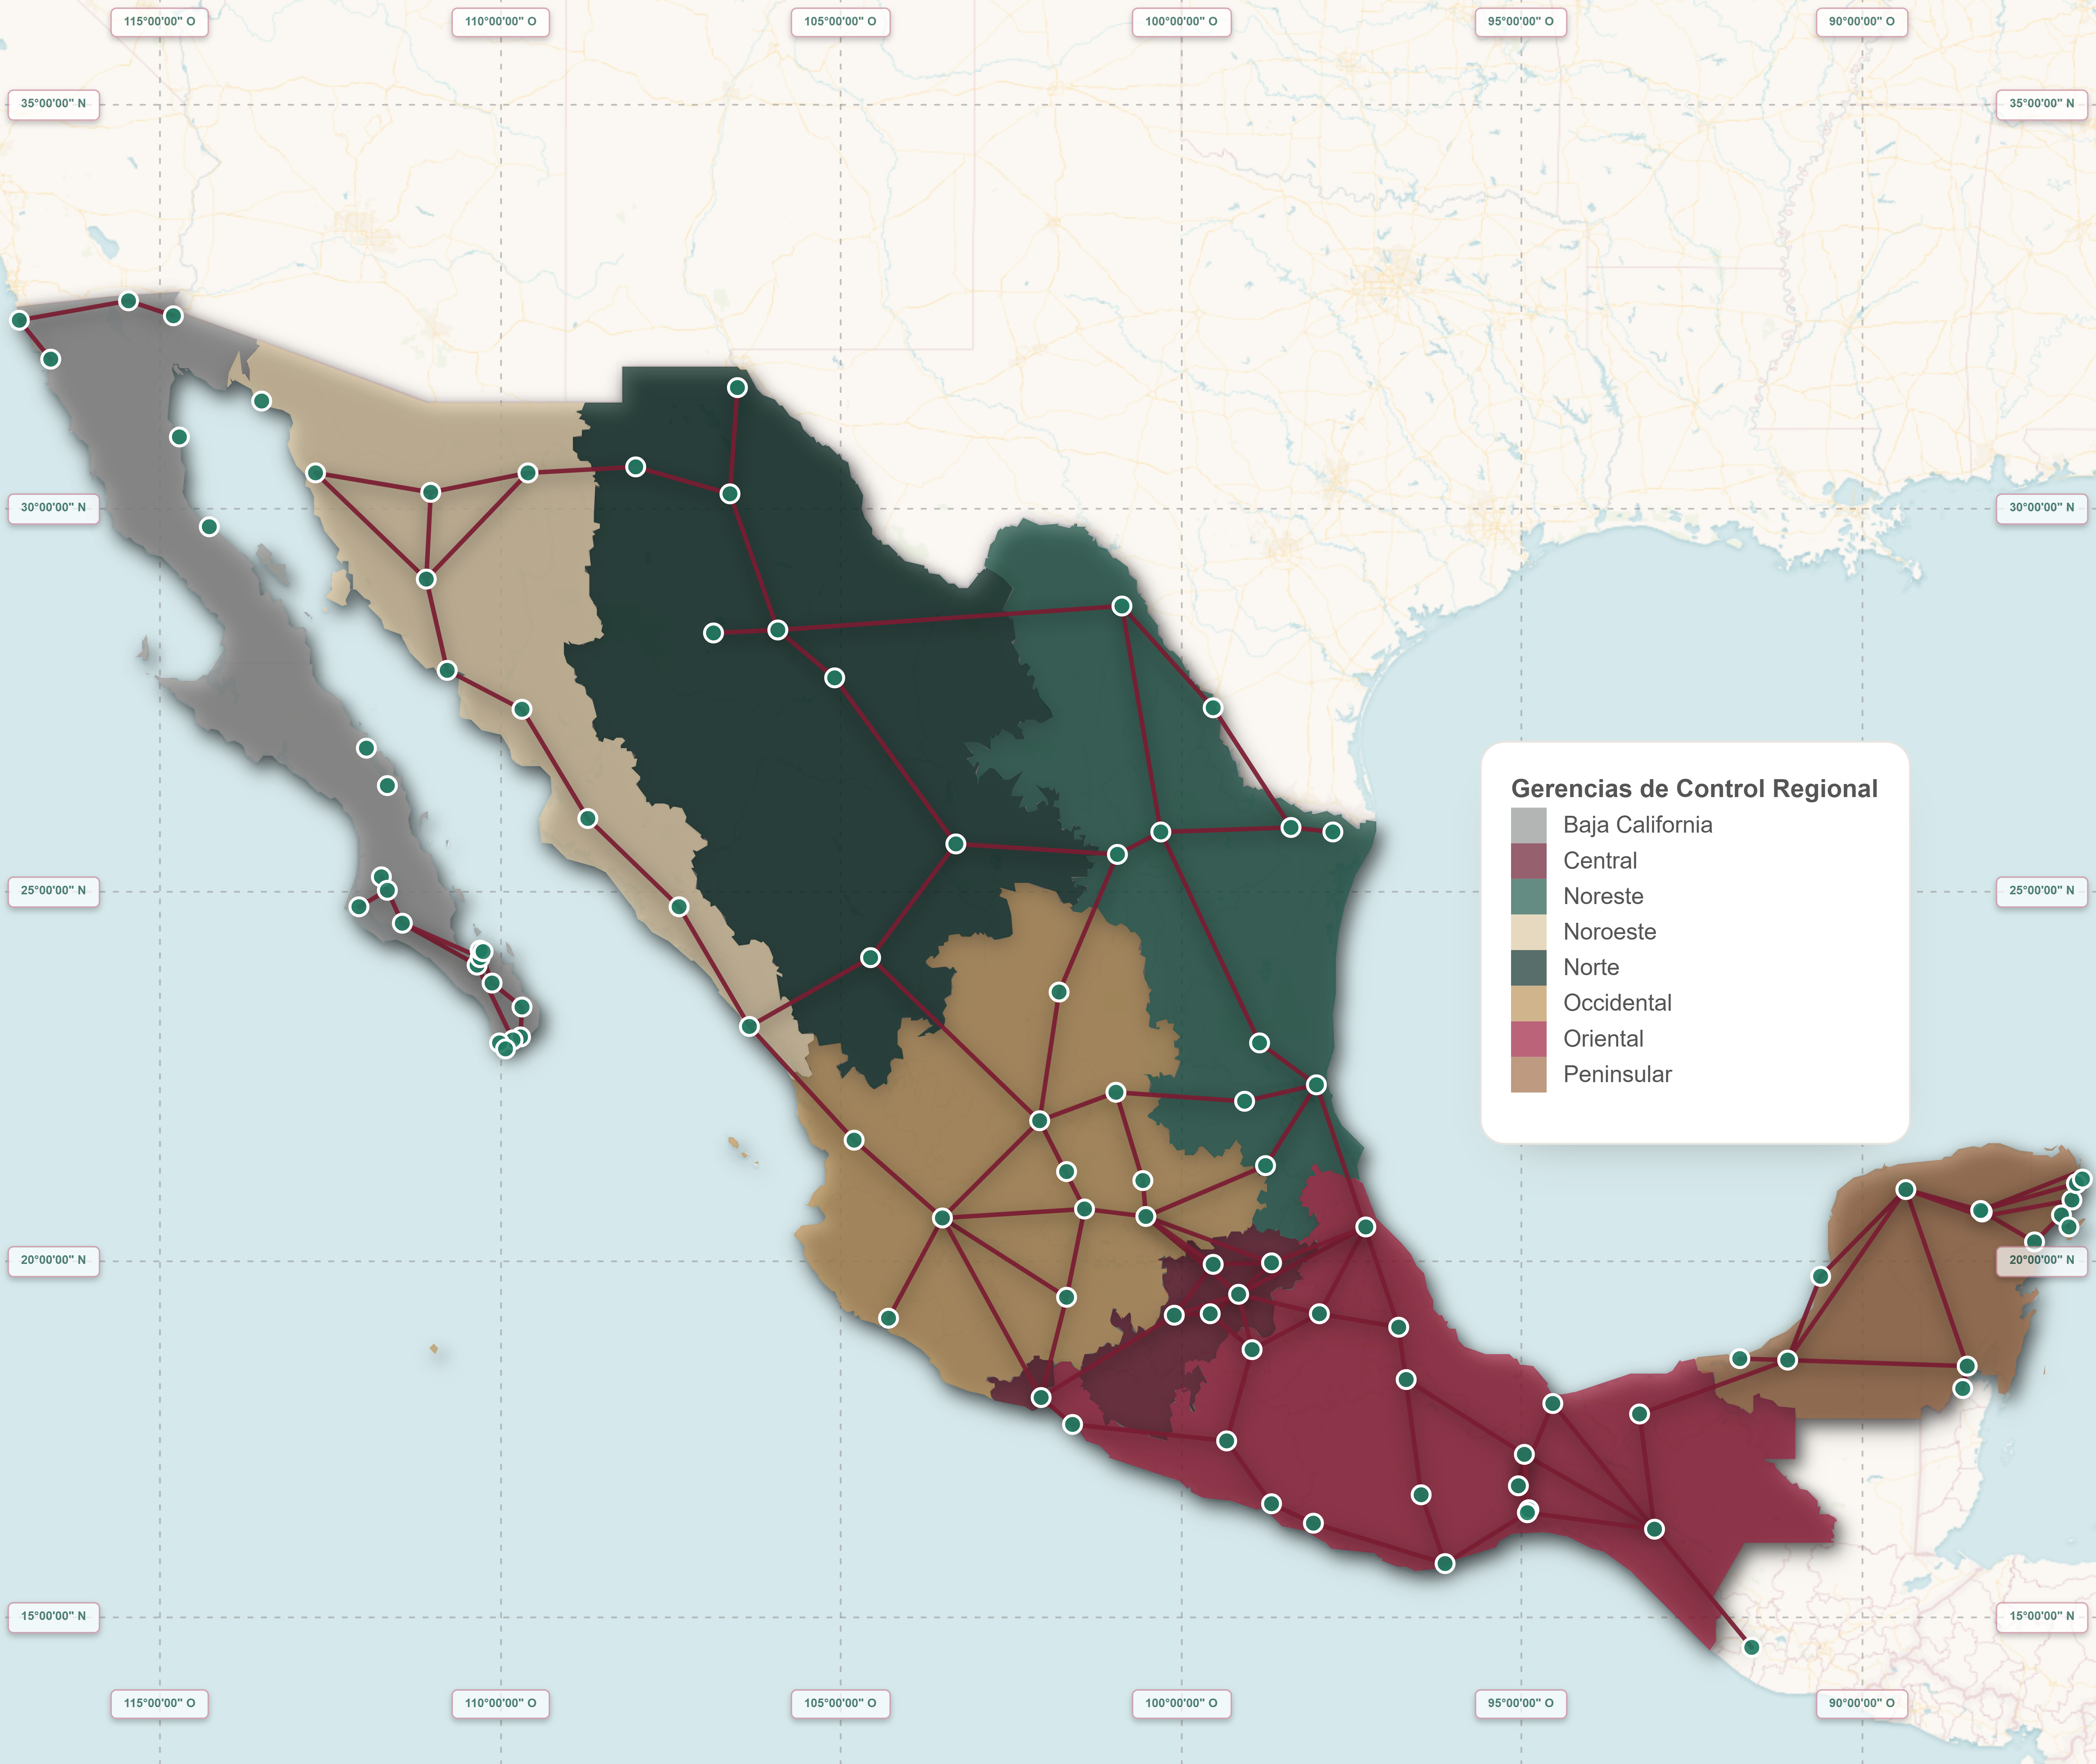
\includegraphics[width=1.0\textwidth]{img/figura_2_1.png}}{Figura 2.1 Principal infraestructura del sector hidrocarburos, 2024}
  \par}
  \raggedright
  \caption{Figura 2.1 Principal infraestructura del sector hidrocarburos, 2024}
  \label{fig:FIG-2.1-1}
\end{figure}
\vspace{-4pt}
\fuente{Elaboración SENER.}



\subsubsection{Exploración y Extracción}

La infraestructura de exploración y extracción está destinada a la localización y obtención de recursos energéticos del subsuelo. Las actividades relacionadas con la exploración y extracción de hidrocarburos se concentran principalmente en las cuencas petroleras de la región marina somera del Golfo de México, así como en la porción terrestre de las cuencas del sureste y noreste del país.

El desarrollo en este sector depende del volumen de reservas de hidrocarburos disponibles, las cuales son certificadas anualmente según su certeza de recuperación. A pesar de que las reservas de hidrocarburos no se consideran parte de la infraestructura petrolera, su localización es el principal objetivo de la exploración petrolera y el punto de partida para la planeación y ejecución de proyectos de extracción.

Las cifras consolidadas al 1 de enero de 2024 para las reservas de aceite, gas, y petróleo crudo equivalente (PCE), agrupadas en las categorías 1P, 2P y 3P\footnote{De acuerdo con el grado de certidumbre, las reservas se clasifican como reserva 1P, la cual es igual a la reserva probada y tienen 90\% de probabilidad de ser extraída bajo las condiciones técnicas y económicas presentes; la reserva 2P es igual a la agregación de reservas probadas más las reservas probables y cuenta con una probabilidad de al menos 50\% de ser extraída bajo las condiciones presentes; y la reserva 3P que es igual a la agregación de las reservas probadas, más las probables más las posibles y tienen al menos 10\% de probabilidades de ser extraídas.} se presentan en la Tabla 2.1.

\begin{tabladoradoCorto}
  \caption{Tabla 2.1 Reservas de Hidrocarburos de la Nación, 2024}
  \label{tab:TBL-2.1.1-1}
  \begin{tabularx}{\textwidth}{Vvvv}
    \toprule
    \rowcolor{gobmxDorado} \encabezadodorado{CATEGORÍA} & \encabezadodorado{ACEITE 
(MMb)} & \encabezadodorado{GAS 
(MMMpc)} & \encabezadodorado{PCE 
(MMbpce)} \\
    \midrule
    Total 1p & 5,978 & 12,297 & 8,383 \\
    Total 2P & 11,078 & 23,302 & 15,530 \\
    Total 3P & 16,383 & 34,858 & 23,146 \\
    \bottomrule
  \end{tabularx}
\end{tabladoradoCorto}
\vspace{-4pt}
\fuente{Elaboración de SENER con información del Sistema de Información de Hidrocarburos de la SENER, Reservas al 01 de enero de 2024}


Es importante destacar que, pese a la disminución de las reservas de hidrocarburos en los últimos años, la tasa de restitución integral de las reservas probadas (1P) de PCE ha permanecido por encima del 100\% desde 2022 hasta 2024.

Las reservas permiten dimensionar el potencial productivo del país, además constituyen un factor estratégico fundamental que incentiva la inversión y promueve el desarrollo del sector energético. Con el objetivo de impulsar el crecimiento de la industria, el Estado Mexicano le otorgó a PEMEX y a empresas privadas los derechos para realizar actividades de exploración o extracción de hidrocarburos, a través de asignaciones y contratos. Las asignaciones fueron otorgadas de manera directa a PEMEX, mientras que los contratos se adjudicaron mediante procesos de licitación en las que participaron tanto empresas privadas como PEMEX. En este contexto, México cuenta con 412 asignaciones operadas por PEMEX, estas asignaciones se distribuyen de la siguiente manera: 314 son terrestres (8 comparten superficie tanto en tierra como en mar), 80 se ubican en aguas someras y 18 en aguas profundas. En cuanto a los contratos (principalmente privados), de los 104 vigentes, 51 se ubican en tierra y 53 son marinos, 30 de aguas someras y 23 de aguas profundas (Tabla 2.2).

Los pozos petroleros hacen posible la exploración, evaluación y producción de petróleo y gas. Durante enero de 2025 se contabilizaron 6,546 pozos operando, de los cuales 3,873 corresponden a pozos de petróleo y gas, y 2,673 a pozos de gas no asociado (Tabla 2.2).

\begin{tabladoradoCorto}
  \caption{Tabla 2.2 Asignaciones, contratos y pozos operando por ubicación, 2024}
  \label{tab:TBL-2.1.1-2}
  \begin{tabularx}{\textwidth}{Vvvv}
    \toprule
    \rowcolor{gobmxDorado} \encabezadodorado{UBICACIÓN} & \encabezadodorado{ASIGNACIONES} & \encabezadodorado{CONTRATOS} & \encabezadodorado{POZOS OPERANDO} \\
    \midrule
    Terrestre & 314 & 51 & 5,924 \\
    Marinos* & 98 & 53 & 622 \\
    Total & 412 & 104 & 6,546 \\
    \bottomrule
  \end{tabularx}
\end{tabladoradoCorto}
\vspace{-4pt}
\fuente{Elaboración de SENER con información del Sistema de Información de Hidrocarburos, Rondas México y Portal de Asignaciones de la SENER\footnote{Incluye aguas someras y profundas}}



\subsubsection{Transformación industrial}

La refinación del petróleo consiste en separar las distintas cadenas de hidrocarburos que lo componen mediante procesos como la destilación, o en modificarlas a través de técnicas como el craqueo o descomposición térmica y catalítica, con el fin de obtener productos específicos, tales como gasolinas, diésel, turbosina y otros derivados.

En México, el Sistema Nacional de Refinación (SNR) está conformado por siete refinerías operadas por PEMEX, las cuales cuentan con una capacidad nominal total de procesamiento de 1,980 Mbd de petróleo crudo (Tabla 2.3).

\begin{tabladoradoCorto}
  \caption{Tabla 2.3 Capacidad de refinación de petróleo crudo en México, 2024}
  \label{tab:TBL-2.1.2-1}
  \begin{tabularx}{\textwidth}{Vvv}
    \toprule
    \rowcolor{gobmxDorado} \encabezadodorado{REFINERÍA} & \encabezadodorado{UBICACIÓN} & \encabezadodorado{Mbd} \\
    \midrule
    Ing. Héctor R. Lara Sosa & Cadereyta, Nuevo León & 275 \\
    Francisco l. Madero & Ciudad Madero, Tamaulipas & 190 \\
    Refinería Olmeca & Dos Bocas, Tabasco & 340 \\
    General Lázaro Cárdenas & Minatitlán, Veracruz & 285 \\
    Ing. Antonio M. Amor & Salamanca, Guanajuato & 245 \\
    Ing. Antonio Dovalí Jaime & Salina Cruz, Oaxaca & 330 \\
    Refinería Miguel Hidalgo & Tula, Hidalgo & 315 \\
    Sistema Nacional de Refinación &  & 1,980 \\
    \bottomrule
  \end{tabularx}
\end{tabladoradoCorto}
\vspace{-4pt}
\fuente{Elaboración de SENER con información del Anuario Estadístico de PEMEX 2024.}


En línea con el objetivo de autosuficiencia energética, a inicios de 2022, con el propósito de fortalecer su participación en el mercado nacional de petrolíferos, PEMEX adquirió el 50\% restante y así obtener el total de la participación en Deer Park Refining Limited Partnership, la cual es una refinería ubicada en Texas, Estados Unidos. A pesar de que la refinería sea propiedad completamente de PEMEX, la producción que llega a México se debe considerar como importada y además tiene que cumplir con las reglas de importación, al ser productos manufacturados fuera del territorio nacional. No obstante, la refinería está produciendo para PEMEX y para los mercados donde tiene influencia, y representa valor a la empresa pública y al Estado mexicano.

En el caso del gas natural extraído del subsuelo, este contiene una mezcla de hidrocarburos que deben ser separados antes de su aprovechamiento. Este proceso se realiza en los Centros Procesadores de Gas (CPG), donde el gas es tratado para separar el metano de otros hidrocarburos más pesados. Como resultado, se obtiene gas seco y líquidos del gas natural, entre los que se encuentran el etano, el gas licuado de petróleo (GLP), las gasolinas naturales y las naftas.

En México operan nueve CPG administrados por PEMEX, los cuales cuentan con una capacidad instalada de 4,283 MMpcd para el endulzamiento\footnote{Proceso de eliminación de impurezas como ácido sulfhídrico (H₂S) y dióxido de carbono (CO₂) del gas natural.} de gas, 135 MMpcd para el tratamiento de líquidos, 5,912 MMpcd para procesos criogénicos, y 560 Mbd para el fraccionamiento de líquidos (Tabla 2.4).

\begin{tabladoradoCorto}
  \caption{Tabla 2.4 Capacidad instalada de Complejos Procesadores de Gas, 2024}
  \label{tab:TBL-2.1.2-2}
  \begin{tabularx}{\textwidth}{Vvvvv}
    \toprule
    \rowcolor{gobmxDorado} \encabezadodorado{COMPLEJO PROCESADOR DE GAS DE PEMEX} & \encabezadodorado{ENDULZAMIENTO DE GAS
  (MMpcd)} & \encabezadodorado{ENDULZAMIENTO DE LÍQUIDOS (Mbd)} & \encabezadodorado{PROCESO CRIOGÉNICO (MMpcd)} & \encabezadodorado{FRACCIONAMIENTO DE LÍQUIDOS (Mbd)} \\
    \midrule
    Burgos & n.a. & n.a. & 1,200 & 18 \\
    Matapionche & 109 & n.a. & 125 & n.a. \\
    CPGP Coatzacoalcos & n.a. & n.a. & 192 & 208 \\
    La Venta & n.a. & n.a. & 182 & n.a. \\
    Nuevo Pemex & 880 & 90 & 1,500 & 208 \\
    Cactus & 1,800 & 45 & 1,275 & 104 \\
    Cd. Pemex & 1,290 & n.a. & 915 & n.a. \\
    Total & 4,283 & 135 & 5,912 & 560 \\
    \bottomrule
  \end{tabularx}
\end{tabladoradoCorto}
\vspace{-4pt}
\fuente{Elaboración de SENER con información de la Dirección General de Gas Natural y Petroquímicos de la SENER. n.a. No aplica.}


La industria petroquímica desempeña un papel fundamental en la transformación de hidrocarburos como el gas natural y sus derivados. México contaba con ocho complejos petroquímicos; sin embargo, debido a políticas gubernamentales anteriores orientadas al abandono del sector y al deterioro de su infraestructura, dos de ellos fueron cerrados. Las razones argumentadas incluyeron la creciente falta de competitividad, el acceso limitado a mercados adecuados y la escasez de materia prima confiable. Estos factores afectaron la rentabilidad al grado de no cubrir ni sus costos variables, por lo que actualmente operan únicamente seis complejos petroquímicos, con una capacidad instalada total de 9,491 Mt (véase Tabla 2.5).

\begin{tabladoradoCorto}
  \caption{Tabla 2.5 Capacidad instalada por Complejos Petroquímicos, 2024}
  \label{tab:TBL-2.1.2-3}
  \begin{tabularx}{\textwidth}{Vvv}
    \toprule
    \rowcolor{gobmxDorado} \encabezadodorado{COMPLEJOS PETROQUÍMICOS} & \encabezadodorado{UBICACIÓN} & \encabezadodorado{CAPACIDAD Mt} \\
    \midrule
    Cosoleacaque & Cosoleacaque, Veracruz. & 4,213 \\
    Independencia & San Martín Texmelucan, Puebla. & 183 \\
    La Cangrejera & Coatzacoalcos, Veracruz. & 2,818 \\
    Morelos & Coatzacoalcos, Veracruz. & 2,277 \\
    Total &  & 9,491 \\
    \bottomrule
  \end{tabularx}
\end{tabladoradoCorto}
\vspace{-4pt}
\fuente{Elaboración de SENER con información del Anuario Estadístico 2024 de PEMEX.}


Como se observa en la tabla 2.6, La Cangrejera y Morelos llevan a cabo procesos petroquímicos diversos como etileno, polietileno, línea de aromáticos, etc. Mientras que Cosoleacaque e Independencia concentran sus procesos en amoniaco, metanol y especialidades petroquímicas.

\begin{tabladoradoCorto}
  \caption{Tabla 2.6 Capacidad nominal por producto de cada Complejos Petroquímicos, 2024}
  \label{tab:TBL-2.1.2-4}
  \begin{tabularx}{\textwidth}{Vvvvv}
    \toprule
    \rowcolor{gobmxDorado} \encabezadodorado{PROCESO (Mt)} & \encabezadodorado{LA CANGREJERA} & \encabezadodorado{COSOLEACAQUE} & \encabezadodorado{MORELOS} & \encabezadodorado{INDEPENDENCIA} \\
    \midrule
    Línea de Aromáticos & 1,342 & 0 & 0 & 0 \\
    Estireno & 150 & 0 & 0 & 0 \\
    Especialidades Petroquímicas & 0 & 0 & 0 & 15 \\
    Metanol & 0 & 0 & 0 & 168 \\
    Etileno & 689 & 0 & 655 & 0 \\
    Polietileno & 315 & 0 & 502 & 0 \\
    Óxido de Etileno & 130 & 0 & 541 & 0 \\
    Oxígeno & 192 & 0 & 483 & 0 \\
    Acrilonitrilo & 0 & 0 & 96 & 0 \\
    Amoniaco & 0 & 4,213 & 0 & 0 \\
    TOTAL & 2,818 & 4,213 & 2,277 & 183 \\
    \bottomrule
  \end{tabularx}
\end{tabladoradoCorto}
\vspace{-4pt}
\fuente{Elaboración de SENER con información del Anuario Estadístico 2024 de PEMEX.}


Frente a esta situación, la política energética vigente ha reorientado sus esfuerzos hacia la recuperación del sector petroquímico como componente central para fortalecer la soberanía energética nacional. En ese sentido, se han diseñado programas de mantenimiento integral y modernización operativa con el objetivo de revitalizar los complejos existentes y consolidar su viabilidad económica.


\subsubsection{Transporte, almacenamiento y distribución}

El gas seco obtenido de los CPG, así como el extraído directo de campos y el importado, puede ser transportado y distribuido hacia los usuarios finales a través de ductos. En 2024 la infraestructura de transporte de gas natural por dicho medio, cuenta con una longitud de 21,149 km, de los cuales 9,732 km (46\%) se encuentran interconectados e integrados al Sistema de Transporte y Almacenamiento Nacional Integrado de Gas Natural (SISTRANGAS), el cual es gestionado por el Centro Nacional de Control del Gas Natural (CENAGAS). Asimismo, el CENAGAS opera y da mantenimiento al Sistema Naco-Hermosillo (SNH), que consta de 355 km. El resto de los gasoductos, son operados y gestionados de forma independiente por privados.

En el SISTRANGAS, de los 9,732 km que lo conforman, 8,386 km (86.2\%) forman parte del Sistema Nacional de Gasoductos (SNG) y son propiedad del Estado, en tanto que 1,346 km de gasoductos son privados (13.8\%) y están interconectados e integrados al SISTRANGAS (Tabla 2.7).

\begin{tabladoradoCorto}
  \caption{Tabla 2.7 Sistemas de transporte de gas seco, 2024}
  \label{tab:TBL-2.1.3-1}
  \begin{tabularx}{\textwidth}{Vvv}
    \toprule
    \rowcolor{gobmxDorado} \encabezadodorado{SISTEMA INTEGRADO} & \encabezadodorado{SISTEMA} & \encabezadodorado{LONGITUD
 (km)} \\
    \midrule
    SISTRANGAS & SNG & 8,386 \\
     & Gasoductos privados interconectados e integrados & 1,346 \\
    SNH & Sistema Naco-Hermosillo & 355 \\
    Total &  & 10,087 \\
    \bottomrule
  \end{tabularx}
\end{tabladoradoCorto}
\vspace{-4pt}
\fuente{Elaboración de SENER con información de CENAGAS.}


Es importante resaltar que el gas seco que se consume en el país se obtiene principalmente por importación. Al cierre de 2024, para la importación de este energético por ducto, se contaban con 24 puntos de internación con la frontera de Estados Unidos. En cuanto al almacenamiento de gas natural, existen 5 terminales de regasificación y almacenamiento de gas natural licuado\footnote{La Agencia Internacional de Energía define el Gas Natural Licuado como una forma de gas natural apta para el transporte marítimo. El gas natural se licúa reduciendo su temperatura a -162 °C a presión atmosférica, lo que reduce sus necesidades de espacio para almacenamiento y transporte en más de 600 veces.} (ver Tabla 2.8).

\begin{tabladoradoCorto}
  \caption{Tabla 2.8 Terminales de almacenamiento y regasificación de gas natural licuado, 2024}
  \label{tab:TBL-2.1.3-2}
  \begin{tabularx}{\textwidth}{Vv}
    \toprule
    \rowcolor{gobmxDorado} \encabezadodorado{UBICACIÓN} & \encabezadodorado{CAPACIDAD DE ALMACENAMIENTO
 (METROS CÚBICOS)} \\
    \midrule
    Pichilingue, Baja California Sur & 145,954 \\
    Aldama, Tamaulipas & 160,683 \\
    Altamira, Tamaulipas & 300,000 \\
    Manzanillo, Colima & 300,000 \\
    Ensenada, Baja California & 320,000 \\
    \bottomrule
  \end{tabularx}
\end{tabladoradoCorto}
\vspace{-4pt}
\fuente{Elaboración de SENER con información de la Unidad de Políticas de Transformación Industrial de SENER}


Mientras que los petrolíferos producidos en las refinerías y los importados a través de las terminales de operación marítima y portuaria, son transportados por ductos, auto tanques, carro tanques o buque tanques para su almacenamiento. En 2024, el transporte de petrolíferos, que considera poliductos, ramales, ductos bidireccionales, entre otros, abarcó una extensión total de 9,582 km y una capacidad de 4,586 Mb. En el caso de GLP, la red existente de 4 ductos en el país suman 2,044 km (Tabla 2.9).

\begin{tabladoradoCorto}
  \caption{Tabla 2.9. Capacidad de transporte por ducto de petrolíferos y gas licuado de petróleo, 2024}
  \label{tab:TBL-2.1.3-3}
  \begin{tabularx}{\textwidth}{Vvv}
    \toprule
    \rowcolor{gobmxDorado} \encabezadodorado{NACIONAL} & \encabezadodorado{LONGITUD (KM)} & \encabezadodorado{CAPACIDAD NOMINAL (MBD)} \\
    \midrule
    Transporte de petrolíferos líquidos 1 & 9,582 & 4,586 \\
    Transporte de gas L.P. 2 & 2,044 & 333 \\
    \bottomrule
  \end{tabularx}
\end{tabladoradoCorto}
\vspace{-4pt}
\fuente{Elaboración de SENER con información de Infraestructura Nacional de Almacenamiento y Transporte por Ducto de Petrolíferos y Prontuario Estadístico de la SENER. \footnote{Infraestructura Nacional de Almacenamiento y Transporte por Ducto de Petrolíferos 2024 de la SENER.} \footnote{Prontuario Estadístico de la SENER.}}


Las Terminales de Almacenamiento y Distribución (TAD) reciben los petrolíferos desde los lugares de producción u origen, para almacenarlos y posteriormente su reparto. El transporte de los petrolíferos desde las TAD para su distribución a los puntos de expendio al público se realiza mediante autotanques propiedad de PEMEX o de empresas privadas. Esto permite suministrar petrolíferos a las estaciones de servicio distribuidas a lo largo y ancho del país. En la Tabla 2.10 se muestran las capacidades de almacenamiento y distribución de petrolíferos.

\begin{tabladoradoCorto}
  \caption{Tabla 2.10. Capacidad de almacenamiento y distribución de Petrolíferos, 2024}
  \label{tab:TBL-2.1.3-4}
  \begin{tabularx}{\textwidth}{Vvv}
    \toprule
    \rowcolor{gobmxDorado} \encabezadodorado{MODALIDAD} & \encabezadodorado{TERMINALES} & \encabezadodorado{CAPACIDAD (MB)} \\
    \midrule
    TAD de Pemex (Terrestres) & 62 & 9,097 \\
    Terminales de operación portuaria & 10 & 4,768 \\
    Terminales de operación marítima & 5 & 8,566 \\
    Terminales de almacenamiento privadas & 15 & 12,772 \\
    Almacenamiento en ASA & 52 & 685 \\
    Almacenamiento de turbosina y gasavión de privados & 4  & 7 \\
    Almacenamiento de turbosina GAFSACOMM & 9 & 149 \\
    Terminales de almacenamiento de CFE & 49 & 10,276 \\
    Distribuidores* & 247 & 1,204 \\
    \bottomrule
  \end{tabularx}
\end{tabladoradoCorto}
\vspace{-4pt}
\fuente{Elaboración de SENER con información del Prontuario Estadístico de la SENER. \footnote{Los Distribuidores son por medios distintos de ductos. ASA: Aeropuertos y Servicios Auxiliares. GAFSACOMM:Grupo Aeroportuario, Ferroviario, de Servicios Auxiliares y Conexos Olmeca-Maya-Mexica.}}


Con la finalidad de contar con instalaciones o sistemas, para conservar en depósito y resguardar el GLP propiedad de terceros, en 2024 se contaba con Plantas de Almacenamiento en México con una capacidad de 6,021 Mb. Además, para adquirir, recibir, guardar y conducir GLP a granel, se cuenta con plantas de distribución para repartición, traslado y enajenación a uno o varios destinos, con una capacidad en 2024 de 2,439 Mb (Ver Tabla 2.11).

\begin{tabladoradoCorto}
  \caption{Tabla 2.11. Capacidad de almacenamiento y distribución de gas licuado de petróleo, 2024}
  \label{tab:TBL-2.1.3-5}
  \begin{tabularx}{\textwidth}{Vvv}
    \toprule
    \rowcolor{gobmxDorado} \encabezadodorado{MODALIDAD} & \encabezadodorado{PERMISOS} & \encabezadodorado{CAPACIDAD (MB)} \\
    \midrule
    Plantas de almacenamiento & 34 & 6,021 \\
    Distribución & 112 & 2,439 \\
    \bottomrule
  \end{tabularx}
\end{tabladoradoCorto}
\vspace{-4pt}
\fuente{Elaboración de SENER con información del Prontuario Estadístico de la SENER.}



\subsection{Infraestructura del Sector Eléctrico}

La infraestructura del Sistema Eléctrico Nacional (SEN) cumple con dos funciones principales que permiten satisfacer la demanda de electricidad en el país: la generación de energía eléctrica para su transmisión y distribución a los centros de consumo. En el país se cuenta con más de 100 GW de capacidad de generación permisionada y más de 100 mil kilómetros en la Red Nacional de Transmisión (RNT), que conectan las principales fuentes de generación con la infraestructura de transformación (193 mil MVA). Asimismo, existen cerca de 900 mil kilómetros en las Redes Generales de Distribución (RGD) que se encargan de llevar la electricidad directamente a hogares, comercios e industrias.

En las siguientes secciones, se describen estos componentes para entender su importancia e integración en la infraestructura del sector eléctrico en el país.


\subsubsection{Capacidad de Generación de Energía Eléctrica}

La generación de electricidad sucede primordialmente a gran escala en centrales que utilizan diversas tecnologías. A lo largo del territorio nacional, existen 101,176 MW de capacidad permisionada en operación a 2024, distribuidos como se muestra en la Figura 2.2.

\Needspace{18\baselineskip}
\begin{figure}[H]
  {\centering
  % Texto alternativo para accesibilidad
  \pdftooltip{\includegraphics[width=1.0\textwidth]{img/figura_2_2.png}}{Figura 2.2 Centrales de generación eléctrica, 2024}
  \par}
  \raggedright
  \caption{Figura 2.2 Centrales de generación eléctrica, 2024
}
  \label{fig:FIG-2.2.1-1}
\end{figure}
\vspace{-4pt}
\fuente{Elaboración SENER.}


Como se observa en la Tabla 2.12, la tecnología de ciclo combinado es la que actualmente tiene una mayor aportación a la capacidad total del SEN, con cerca de 41 GW; seguida de la térmica convencional con 15 GW y la hidroeléctrica con 13 GW aproximadamente.

\begin{tabladoradoCorto}
  \caption{Tabla 2.12. Capacidad permisionada en operación, 2024}
  \label{tab:TBL-2.2.1-1}
  \begin{tabularx}{\textwidth}{Vv}
    \toprule
    \rowcolor{gobmxDorado} \encabezadodorado{TECNOLOGÍA} & \encabezadodorado{CAPACIDAD (MW)} \\
    \midrule
    Carboeléctrica & 5,498 \\
    Ciclo Combinado & 40,858 \\
    Cogeneración Eficiente & 2,028 \\
    Combustión Interna & 1,032 \\
    Eólica & 7,388 \\
    Geotérmica & 997 \\
    Hidroeléctrica & 12,875 \\
    Nucleoeléctrica & 1,634 \\
    Solar Fotovoltaica & 8,546 \\
    Termoeléctrica Convencional & 15,143 \\
    Turbogas & 4,590 \\
    Otras & 587 \\
    \bottomrule
  \end{tabularx}
\end{tabladoradoCorto}
\vspace{-4pt}
\fuente{Elaboración de SENER con información de la CRE* al 31 de diciembre de 2024. \footnote{Actualmente la Comisión Nacional de Energía (CNE), de acuerdo con la publicación de la Ley de la Comisión Nacional de Energía el 18 de marzo de 2025, que abroga la Ley de los Órganos Reguladores Coordinados en Materia de Energía}.}



\subsubsection{Transmisión y Disitribución}

Comparada con una extensa red de carreteras que transporta la electricidad desde las plantas de generación eléctrica, la RNT está integrada por más de 100 mil kilómetros de líneas de alta tensión que recorren el territorio del país. La Tabla 2.13 describe los dos grandes grupos de niveles de tensión para el año 2024: el primero, dedicado a la transmisión de entre 161 a 400 kV con 56,409 km, donde destacan las líneas de 400 kV (26,135 km) y 230 kV (29,743 km) para el transporte de energía eléctrica a gran escala; el segundo grupo, de 69 a 138 kV con 54,437 km, donde predominan líneas de 115 kV (48,725 km) que son vías primarias para la distribución regional y la interconexión de subestaciones. Esta infraestructura de 110,846 km, refleja la columna vertebral del sistema eléctrico mexicano.

\begin{tabladoradoCorto}
  \caption{Tabla 2.13. Longitud de las líneas de transmisión de la  Red Nacional de Transmisión, 2024}
  \label{tab:TBL-2.2.2-1}
  \begin{tabularx}{\textwidth}{Vv}
    \toprule
    \rowcolor{gobmxDorado} \encabezadodorado{NIVEL DE TENSIÓN} & \encabezadodorado{LONGITUD (KM)} \\
    \midrule
    Transmisión entre 161 y 400 kV & 56,200 \\
    400 kV & 26,135 \\
    230 kV & 29,743 \\
    161 kV & 531 \\
    Transmisión entre 69 y 138 kV & 54,939 \\
    138 kV & 1,620 \\
    115 kV & 48,725 \\
    85 kV & 1,757 \\
    69 kV & 2,335 \\
    TOTAL & 110,846 \\
    \bottomrule
  \end{tabularx}
\end{tabladoradoCorto}
\vspace{-4pt}
\fuente{Elaboración de SENER con información de CENACE y CFE al 31 de diciembre de 2024.}


Entre la RNT y la distribución a centros de consumo, se encuentra la infraestructura de transformación, es decir, los equipos de acondicionamiento de la corriente transportada según las necesidades de la infraestructura de transporte. Para 2024, se cuenta con una capacidad de 113,688 MVA en bancos de transformación. La Tabla 2.14 muestra la capacidad de transformación en la RNT y las RGD del MEM (subestaciones de alta a media tensión que forman parte del Mercado Eléctrico Mayorista).

\begin{tabladoradoCorto}
  \caption{Tabla 2.14. Capacidad de transformación en la  Red Nacional de Transmisión, 2024}
  \label{tab:TBL-2.2.2-2}
  \begin{tabularx}{\textwidth}{Vv}
    \toprule
    \rowcolor{gobmxDorado} \encabezadodorado{NIVEL DE TENSIÓN} & \encabezadodorado{CAPACIDAD DE TRANSFORMACIÓN (MVA) 2024} \\
    \midrule
    Bancos de Transformación de la RNT & 113,688 \\
    Bancos de Transformación de las RGD del MEM & 79,812 \\
    TOTAL & 193,500 \\
    \bottomrule
  \end{tabularx}
\end{tabladoradoCorto}
\vspace{-4pt}
\fuente{Elaboración de SENER con información de CENACE.}


Por otra parte, las RGD que entregan la electricidad a los usuarios finales, se componen de líneas de media tensión (2.4 - 34 kV), baja tensión (menos de 2.4 kV), así como de capacidad de transformación. En la Tabla 2.15 se muestra la infraestructura de distribución de energía eléctrica registrada en 2024.

\begin{tabladoradoCorto}
  \caption{Tabla 2.15. Características de las líneas de distribución de las Redes Generales de Distribución, 2024}
  \label{tab:TBL-2.2.2-3}
  \begin{tabularx}{\textwidth}{Vv}
    \toprule
    \rowcolor{gobmxDorado} \encabezadodorado{INFRAESTRUCTURA DE DISTRIBUCIÓN} & \encabezadodorado{2024} \\
    \midrule
    Longitud de líneas de media tensión en distribución (km) 2.4 a 34 kV & 555,336 \\
    Longitud de líneas de baja tensión en distribución (km) menor a 2.4 kV & 345,966 \\
    Capacidad Instalada en redes de distribución (MVA) & 64,894 \\
    Transformadores en Redes de distribución de media a baja tensión & 1,805,396 \\
    \bottomrule
  \end{tabularx}
\end{tabladoradoCorto}
\vspace{-4pt}
\fuente{Elaboración de SENER con información de CFE.}



\subsubsection{Capacidad Instalada de Generación Distribuida}

De conformidad con el artículo 3, fracción XXII de la Ley del Sector Eléctrico (LSE), la Generación Distribuida (GD) es la generación que se realiza por una Generadora Exenta y que se encuentra interconectada a un circuito de distribución que contenga una alta concentración de Centros de Carga. Cabe señalar, que el artículo 19 de la LSE establece que todas las Centrales Eléctricas con capacidad menor a 0.7 MW son Generadoras Exentas\footnote{Bajo el marco legislativo de la abrogada Ley de la Industria Eléctrica (LIE), este límite era de 0.5 MW}. En otras palabras, la GD es la generación de energía eléctrica a través de centrales eléctricas de pequeña escala (Generadoras Exentas), que no requieren ni cuentan con un permiso de generación otorgado por la autoridad reguladora, pero puede estar interconectada a un circuito de distribución. Generalmente, estas centrales se encuentran cerca del punto de consumo y abastecen parcial o totalmente la demanda local.

Al cierre de 2024, la Comisión Reguladora de Energía\footnote{Ahora la Comisión Nacional de Energía} registró un crecimiento de la capacidad instalada de la GD cercana al 30\% con respecto al año anterior, resultando en 4,447.92 MW, bajo las figuras de Generador Exento de la anterior Ley de la Industria Eléctrica (LIE), y los Contratos de Interconexión de Pequeña y Mediana Escala, de la la antigua Ley del Servicio Público de Energía Eléctrica (LSPEE) (Tabla 2.16).

\begin{tabladoradoCorto}
  \caption{Tabla 2.16. Capacidad Instalada acumulada de Generación Distribuida, 2024}
  \label{tab:TBL-2.2.3-1}
  \begin{tabularx}{\textwidth}{V}
    \toprule
    \rowcolor{gobmxDorado} \encabezadodorado{Capacidad instalada de Generación distribuida} \\
    \midrule
    Total (MW) \\
    Contratos (n°) \\
    \bottomrule
  \end{tabularx}
\end{tabladoradoCorto}
\vspace{-4pt}
\fuente{Elaboración propia con información de CRE.}


Si bien, cualquier tipo de tecnología de generación puede ser aplicada a una Central Eléctrica de GD, la capacidad que actualmente se encuentra instalada predominantemente es de tecnología solar fotovoltaica, con una participación de 99.41\% del total. Lo que deja al resto de las tecnologías (eólica, bioenergía y otras) con una participación de apenas el 0.59\% en su conjunto. Como se puede observar en la Figura 2.3, Jalisco y Nuevo León son las entidades federativas que concentran cerca del 25\% de la capacidad instalada en la República Mexicana.

\Needspace{18\baselineskip}
\begin{figure}[H]
  {\centering
  % Texto alternativo para accesibilidad
  \pdftooltip{\includegraphics[width=1.0\textwidth]{img/figura_2_3.png}}{Figura 2.3 Capacidad de Generación distribuida por Estado, 2024}
  \par}
  \raggedright
  \caption{Figura 2.3 Capacidad de generación distribuida por Estado, 2024}
  \label{fig:FIG-2.2.3-1}
\end{figure}
\vspace{-4pt}
\fuente{Elaboración SENER.}



\subsection{Infraestructura de consumo final y aprovechamiento directo}

La infraestructura de consumo final está compuesta por el conjunto de equipos, vehículos, edificaciones, instalaciones y sistemas que utilizan energéticos para realizar funciones productivas, de transporte, comerciales, residenciales o de servicios. Esta composición es reflejo de la diversidad sectorial y territorial del país, por lo que su caracterización es clave para el análisis de los patrones de consumo.

En el sector transporte, que representa el mayor componente del consumo final energético nacional (45.59\% en 2024), la modalidad define la participación que tendrá en el consumo de energía. El transporte terrestre (automóviles particulares, taxis, motocicletas, camionetas de reparto, autobuses de pasajeros y camiones de carga), está dominado por un parque vehicular en circulación que se estima cercano a 50 millones de unidades\footnote{Vehículos de Motor Registrados en Circulación (VMRC) del INEGI, 2025.}. La infraestructura ferroviaria, aunque más limitada, cuenta con más de 1,300 locomotoras en operación, con más de 160 vagones para el transporte de pasajeros y más de 30 mil carros para carga (incluyendo plataformas, tolvas y vagones especializados)\footnote{Anuario estadístico ferroviario de SICT, 2024.}. El transporte marítimo y fluvial utiliza embarcaciones de carga, ferrys y lanchas de transporte local en ríos y costas. En el transporte aéreo, el consumo energético se concentra en aeronaves comerciales y de carga que operan con turbosina, con una flota nacional de aproximadamente 5,200 aeronaves activas\footnote{Anuario estadístico del sector infraestructura, comunicaciones y transportes de SICT, 2023.}.

El sector industrial contaba con más de 640 mil unidades económicas\footnote{Códigos SCIAN: 21, 23, 31, 32 y 33. Directorio Estadístico Nacional de Unidades Económicas del INEGI, 2025.}, en 2024, con patrones de consumo altamente diferenciados según la rama productiva. La minería, cementera, siderurgia y metalurgia y la producción de papel se caracterizan por utilizar maquinaria pesada, hornos, calderas, intercambiadores de calor, sistemas de bombeo, ventilación y compresión, así como infraestructura para climatización e iluminación. En cambio, otras industrias como la química, alimentaria, textil o automotriz concentran su demanda en operaciones de maquinado, refrigeración, climatización y procesos específicos.

El sector comercio y servicios integra una infraestructura energética amplia, debido a la cantidad de unidades económicas existentes (más de 2,600,000 en 2024)\footnote{Códigos SCIAN: 72, 52,53, 54, 55, 56, 71, 81, 93, 61 y 62. Directorio Estadístico Nacional de Unidades Económicas del INEGI, 2025.}. Además, grandes edificios corporativos, instituciones de salud y educación, y oficinas de la administración pública, requieren un suministro energético constante para mantener condiciones adecuadas de operación, seguridad y confort.

El consumo en el sector residencial está directamente ligado al número de viviendas, la cantidad de habitantes por hogar y la penetración de electrodomésticos, tecnologías y dispositivos para satisfacer necesidades energéticas y confort. Según datos del INEGI, en 2020, de las más de 33 millones de viviendas particulares habitadas, casi el 99\% contó con suministro de energía eléctrica; y un promedio de 66\% contó con diversos electrodomésticos\footnote{Censo de Población y Vivienda 2020 del INEGI, 2021.}. En los hogares, la infraestructura de consumo incluye una vasta gama de dispositivos eléctricos (refrigeradores, lavadoras, televisores, equipos de cómputo), y equipamiento para iluminación, calentamiento de agua, cocción de alimentos y climatización (aires acondicionados y calefactores de espacios).

En cuanto al sector público, existen dos tipos de infraestructura energética relevantes. El alumbrado público, con más de 9 millones de luminarias en funcionamiento a lo largo del territorio nacional\footnote{Censo Nacional de Gobiernos Municipales y Demarcaciones Territoriales de la Ciudad de México 2023.}, representa un componente esencial del consumo eléctrico municipal. En paralelo, los sistemas de bombeo y tratamiento de agua potable y residual dependen de la electricidad para su funcionamiento continuo. Estos sistemas son operados principalmente por los más de 2,500 organismos públicos\footnote{Censos Económicos (CE) publicado en 2024 por el INEGI.}; aunque también existen cerca de 2,270 prestadores de servicio de agua de gestión social o privada\footnote{Censo Nacional de Gobiernos Municipales y Demarcaciones Territoriales de la Ciudad de México 2023, INEGI.}.

Por su parte, el sector agropecuario utiliza una variada infraestructura de consumo esencial para la producción de alimentos. Entre los equipos destacan los tractores, cosechadoras y sembradoras y sistemas de riego. Mientras que para los procesos de post-cosecha, se usan secadores, molinos y equipos de refrigeración para almacenamiento de alimentos. Para la industria producción pecuaria, se utilizan equipos de ventilación, sistemas de alimentación automática, ordeñadoras eléctricas y calentadores.

Además, en México, los sistemas de aprovechamiento energético directo representan una alternativa eficiente y adecuada para diversos sectores productivos. Entre ellos, destacan particularmente los calentadores solares de agua (CSA), cuya adopción ha crecido significativamente en los últimos años. Según datos de Fabricantes Mexicanos de Energías Renovables, A.C. a 2024, el país cuenta con una capacidad instalada mayor a los 4,800 MW\footnote{Equivalentes a aproximadamente 7 millones de metros cuadrados de colectores solares.} térmicos que representa un crecimiento del 34\% con respecto a lo instalado en el 2020 (SECIHTI, 2022). Esta tecnología se implementa principalmente en viviendas, aunque también ha tenido un crecimiento importante en establecimientos hoteleros, centros hospitalarios, gimnasios y procesos industriales, durante los últimos 15 años.


\portadaseccion{3}{Oferta interna bruta}{}

\section{Oferta interna bruta}

En este capítulo se presentan los elementos que componen la oferta interna bruta de energía, entendida como la totalidad de la energía primaria y secundaria disponible para el consumo en un año dado, en este caso el 2024. Metodológicamente, la oferta interna bruta es la suma algebraica de la producción nacional de energía, las importaciones, la variación de inventarios, la energía no aprovechada y las exportaciones de energéticos.


\subsection{Producción de energía primaria}

En 2024, la producción de energía primaria fue de 7,359 PJ y se basó en su mayoría en combustibles fósiles, los cuales representaron cerca del 84\% de la matriz energética, mientras que el restante 16\% se generó a partir de fuentes limpias y renovables. En la Figura 3.1, se presenta la participación de cada energético en el total de la producción de energía primaria en 2024.

\Needspace{18\baselineskip}
\begin{figure}[H]
  {\centering
  % Texto alternativo para accesibilidad
  \pdftooltip{\includegraphics[width=1.0\textwidth]{img/figura_3_1.png}}{Figura 3.1 Estructura porcentual de la producción de energía primaria por energético, 2024}
  \par}
  \raggedright
  \caption{Figura 3.1 Estructura porcentual de la producción de energía primaria por energético, 2024}
  \label{fig:FIG-3.1-1}
\end{figure}
\vspace{-4pt}
\fuente{Elaboración SENER.}


Como se muestra en la figura anterior, en 2024, el petróleo crudo representó el 49.7\% de la producción total de energía primaria, por lo que el crudo sigue siendo la base de la matriz energética mexicana. El gas natural ocupó el segundo lugar con 25.4\% y su participación refleja la creciente importancia de este energético como sustituto de derivados del petróleo en la generación de electricidad y como insumo industrial.

En ese mismo año, los condensados alcanzaron una participación de 8.7\% consolidándose como la tercera fuente primaria en importancia. Su incremento en los últimos años responde a la explotación de campos donde se extraen líquidos de gas natural y al enfoque de fortalecer la autosuficiencia en insumos para refinación. Esto marca un cambio significativo, ya que anteriormente su participación en la estructura energética nacional era marginal. En cambio, el carbón mineral sólo tuvo una participación del 0.2\% en la producción energética primaria en el país, lo que destaca a nivel mundial, ya que en países como China, India o Estados Unidos, el carbón es un recurso mucho más relevante para su producción de energía.

Entre 2010 y 2024 (Ver Figura 3.2), la producción de energía primaria en México ha mostrado una tendencia general decreciente, con cambios significativos en la participación de los distintos energéticos en la estructura de la matriz energética. Este comportamiento responde a factores internos como disminución en la producción petrolera además de la reforma energética de 2013\footnote{DECRETO por el que se reforman y adicionan diversas disposiciones de la Constitución Política de los Estados Unidos Mexicanos, en Materia de Energía. Diario Oficial de la Federación. 20/12/2013}, que se tradujo en una política de ceder la exploración y extracción a empresas privadas, mediante contratos que no fueron productivos por la falta de inversión de estas empresas. Entre los factores externos, destacan los cambios en los precios internacionales de los hidrocarburos, un creciente uso de energías provenientes de fuentes renovables y los impactos económicos de eventos globales.

\Needspace{18\baselineskip}
\begin{figure}[H]
  {\centering
  % Texto alternativo para accesibilidad
  \pdftooltip{\includegraphics[width=1.0\textwidth]{img/figura_3_2.png}}{Figura 3.2 Evolución de la producción de energía primaria por energético, 2010-2024}
  \par}
  \raggedright
  \caption{Figura 3.2 Evolución de la producción de energía primaria por energético, 2010-2024}
  \label{fig:FIG-3.1-2}
\end{figure}
\vspace{-4pt}
\fuente{Elaboración SENER.}


En 2010, la producción primaria estaba fuertemente dominada por el petróleo crudo, que generaba 5,937 PJ. Sin embargo, a lo largo de la década siguiente, el petróleo crudo experimentó una disminución en su producción debido a factores propios de los yacimientos existentes. Para 2024, la producción de este energético alcanzó la cantidad de 3,654 PJ, lo que equivale a una disminución del 38.4\%, en relación con la producción de 2010.

La producción de gas natural, por su parte, también tuvo un decrecimiento, pasando de 2,965 PJ en 2010 a 1,868 PJ en 2024; tan sólo de 2023 a 2024 la producción de gas natural disminuyó 8.1\%. Este descenso se debe a la creciente dependencia de importaciones desde Estados Unidos provenientes principalmente de la producción de gas shale.

El declive de la producción de gas natural se vio acelerado por la caída de la inversión total en PEMEX, durante 2012 a 2018, con una tasa anual del -12\%, a diferencia de la inversión total experimentada durante 2000 a 2006 que creció a una tasa anual de 11.8\%. La caída de la inversión se agudizó en 2015, hasta alcanzar su mínimo histórico en 2018\footnote{Plan de negocios de petróleos mexicanos y sus empresas productivas subsidiarias 2019-2023}. Además, esta inversión se destinó prioritariamente a la explotación de los campos petroleros, con alrededor del 85\% de los recursos, mientras que el 15\% restante fue asignado a la exploración de nuevos yacimientos de hidrocarburos.

Esto también justificó el incremento en las importaciones de gas natural desde Estados Unidos, lo cual plantea un desafío estratégico para la seguridad energética del país. En este sentido, el cambio de política energética en 2019, enfocado al rescate de PEMEX y de CFE, tiene como objetivo desarrollar una estrategia con un mayor énfasis en la soberanía y seguridad energética. A partir del rescate de PEMEX y CFE, se busca disminuir la dependencia energética del exterior e incrementar la autosuficiencia para cubrir la demanda nacional en esta materia.

Con respecto a los condensados, éstos crecieron de manera sostenida, sobre todo a partir de 2020, llegando a 721 PJ en 2023. Este incremento se debe al desarrollo de campos petroleros como Ixachi y Quesqui, aunado a la estrategia de PEMEX de aprovechar la producción de campos donde la extracción de crudo se complementa con líquidos del gas natural, así como con la búsqueda de insumos para el SNR. Sin embargo, de 2023 a 2024, la producción de condensados reporta una disminución de 11.5\%.

Por otro lado, las energías limpias y renovables, aunque en términos absolutos han tenido una participación reducida frente a los hidrocarburos en la producción primaria de energía, han mostrado un crecimiento constante. La energía solar pasó de representar el 0.1\% en 2010 a 3.4\% en 2024, con una tasa de incremento anual de 22.5\% en su producción; mientras que la energía eólica pasó de ser también 0.1\% en 2010 a 3\% en 2024, con un crecimiento de más del 21\%.

En tanto que la energía hidráulica pasó de representar el 4.2\% en 2010 a 3.6\% en 2024, se destaca que entre el año 2023 y 2024 tuvo un incremento del 15.5\%. Es importante mencionar que, aunque la energía hidráulica cuenta con un importante potencial de aporte energético, su producción está ligada a los ciclos hidrometeorológicos. Los periodos de sequía en el país han provocado que disminuya su participación en la matriz energética durante los últimos 15 años con una reducción del 3.4\% anual.

Por su parte, la energía nuclear se ha mantenido relativamente estable, dado que no ha habido proyectos de nuevas centrales nucleares.

Los biocombustibles (biogás, bagazo de caña y la leña) continúan con pequeñas aportaciones, principalmente vinculados a sectores específicos como la agroindustria y comunidades rurales. Si bien su importancia en la matriz total es limitada, representan una fuente descentralizada y de carácter estratégico para ciertas regiones del país.

Finalmente, la energía geotérmica ha tenido una disminución importante en su producción energética en los últimos 15 años (51.4\%), aunque su particupación pasó de 1.7\% en 2010 a 1.2\% en 2024.

En resumen, al cierre de 2024, la producción primaria de energía sigue dependiendo mayoritariamente de hidrocarburos como el petróleo crudo y el gas natural, los cuales representaron el 75\% de la matriz de producción primaria de energía. La tendencia indica una diversificación gradual, con un mayor peso relativo en condensados y energías renovables. No obstante, la producción total nacional se encuentra por debajo de los niveles alcanzados en 2010, lo que plantea desafíos en términos de seguridad energética y transición hacia fuentes de energía más limpias.


\subsection{Comercio exterior de energía}

Los datos de la balanza comercial son un referente para analizar el estado de la autosuficiencia energética nacional. El estado actual de las importaciones y exportaciones de energía primaria y secundaria destaca, debido a que en la mayoría de los casos se cuenta con una balanza comercial deficitaria\footnote{El saldo de la balanza comercial neta se obtiene de restar exportaciones menos las importaciones anuales totales.} (Ver Figura 3.3). Sin embargo, en la balanza comercial del petróleo crudo, combustóleo y energía eléctrica se tiene un superávit, como se puede observar en la Figura 3.3. Entre ellos, destaca el superávit comercial de petróleo crudo, el cual tiene un saldo positivo de 1,859.80 PJ, mientras que los saldos netos para el combustóleo y la energía eléctrica son de 496.61 PJ y a 6.94 PJ, respectivamente.

Si bien México es autosuficiente y superavitario con respecto al petróleo crudo, es dependiente de la importación de otros energéticos, como el gas seco, las gasolinas y naftas, así como el diésel. Pese a que el gas natural es el segundo energético más producido en el país, su energético secundario derivado de procesos de transformación, el gas seco es el de mayor importación, con un saldo negativo en su balanza comercial de -2,569.47 PJ. Seguido de petrolíferos como gasolinas y naftas (-1,079.52 PJ) y el diésel (-509.09PJ), pese a que como se mencionó anteriormente, el país es superavitario en petróleo crudo.

Destaca que el gas seco, las gasolinas y naftas, y el diésel son imprescindibles para la generación de energía eléctrica, calentamiento de agua, cocción y la movilidad terrestre de la población y las mercancías. Ello sirve de referente para identificar los energéticos sobre los cuales se deberían enfocar esfuerzos que promuevan la soberanía energética del país.

\Needspace{18\baselineskip}
\begin{figure}[H]
  {\centering
  % Texto alternativo para accesibilidad
  \pdftooltip{\includegraphics[width=1.0\textwidth]{img/figura_3_3.png}}{Figura 3.3 Composición de la balanza comercial de energía por energético, 2024}
  \par}
  \raggedright
  \caption{Figura 3.3 Composición de la balanza comercial de energía por energético, 2024}
  \label{fig:FIG-3.2-1}
\end{figure}
\vspace{-4pt}
\fuente{Elaboración SENER.}



\subsection{Variación de inventarios}

La variación de inventarios se refiere a la diferencia entre la existencia inicial (1° de enero del año en cuestión) y la existencia final (31 de diciembre del mismo año) de productos energéticos almacenados. Un saldo positivo indica que ha aumentado el inventario, en contraposición, un saldo negativo significa que los inventarios de energía han disminuido.

En 2024, el valor la variación de inventarios total fue de -14.72 PJ, esto se debió a una ligera reducción de inventarios de energía.

\Needspace{18\baselineskip}
\begin{figure}[H]
  {\centering
  % Texto alternativo para accesibilidad
  \pdftooltip{\includegraphics[width=1.0\textwidth]{img/figura_3_4.png}}{Figura 3.4 Composición de la variación de inventarios por energético, 2024}
  \par}
  \raggedright
  \caption{Figura 3.4 Composición de la variación de inventarios por energético, 2024}
  \label{fig:FIG-3.3-1}
\end{figure}
\vspace{-4pt}
\fuente{Elaboración SENER.}


Como se muestra en la Figura 3.4, el gas natural fue el combustible con mayor variación de inventarios con -14.07 PJ, seguido por las gasolinas y naftas con una variación de -5.58 PJ y el diesel con -2.98 PJ. Es preciso señalar que, los saldos negativos de gasolinas, naftas y diesel tienen un impacto mínimo en la oferta total de energía, si se considera que en 2023 y 2022 la acumulación de inventarios de estos combustibles fue de -39.51 PJ y -30.28 PJ, respectivamente.


\subsection{Oferta total}

En 2024, la oferta total de energía en el país alcanzó 12,353.61 PJ. Esto es, la sumatoria de la producción, importación y la variación de inventarios, tanto de energía primaria como secundaria\footnote{Si bien se trata de una sumatoria, en la contabilización de los flujos energéticos, la producción se registra con un signo positivo, ya que significa una entrada, las importaciones con signo positivo por su procedencia del extranjero, mientras que el signo de la variación de inventarios dependerá del resultado de la resta que implica su cálculo. De modo que, al realizar la suma, el resultado de la oferta total de energía dependerá de los signos de las variables.}. Esta información es esencial para calcular la oferta interna bruta nacional. Como se muestra en la Figura 3.5, los principales energéticos que forman parte de la oferta total de energía son: petróleo crudo (29.7\%), los condensados (5.2\%), el gas natural (15\%), el gas seco (20.9\%), gasolinas y naftas (8.7\%), y el diésel (4.4\%). Lo anterior, resalta que el 90.23\% de la oferta total de energía en México proviene de fuentes fósiles, principalmente hidrocarburos.

\Needspace{18\baselineskip}
\begin{figure}[H]
  {\centering
  % Texto alternativo para accesibilidad
  \pdftooltip{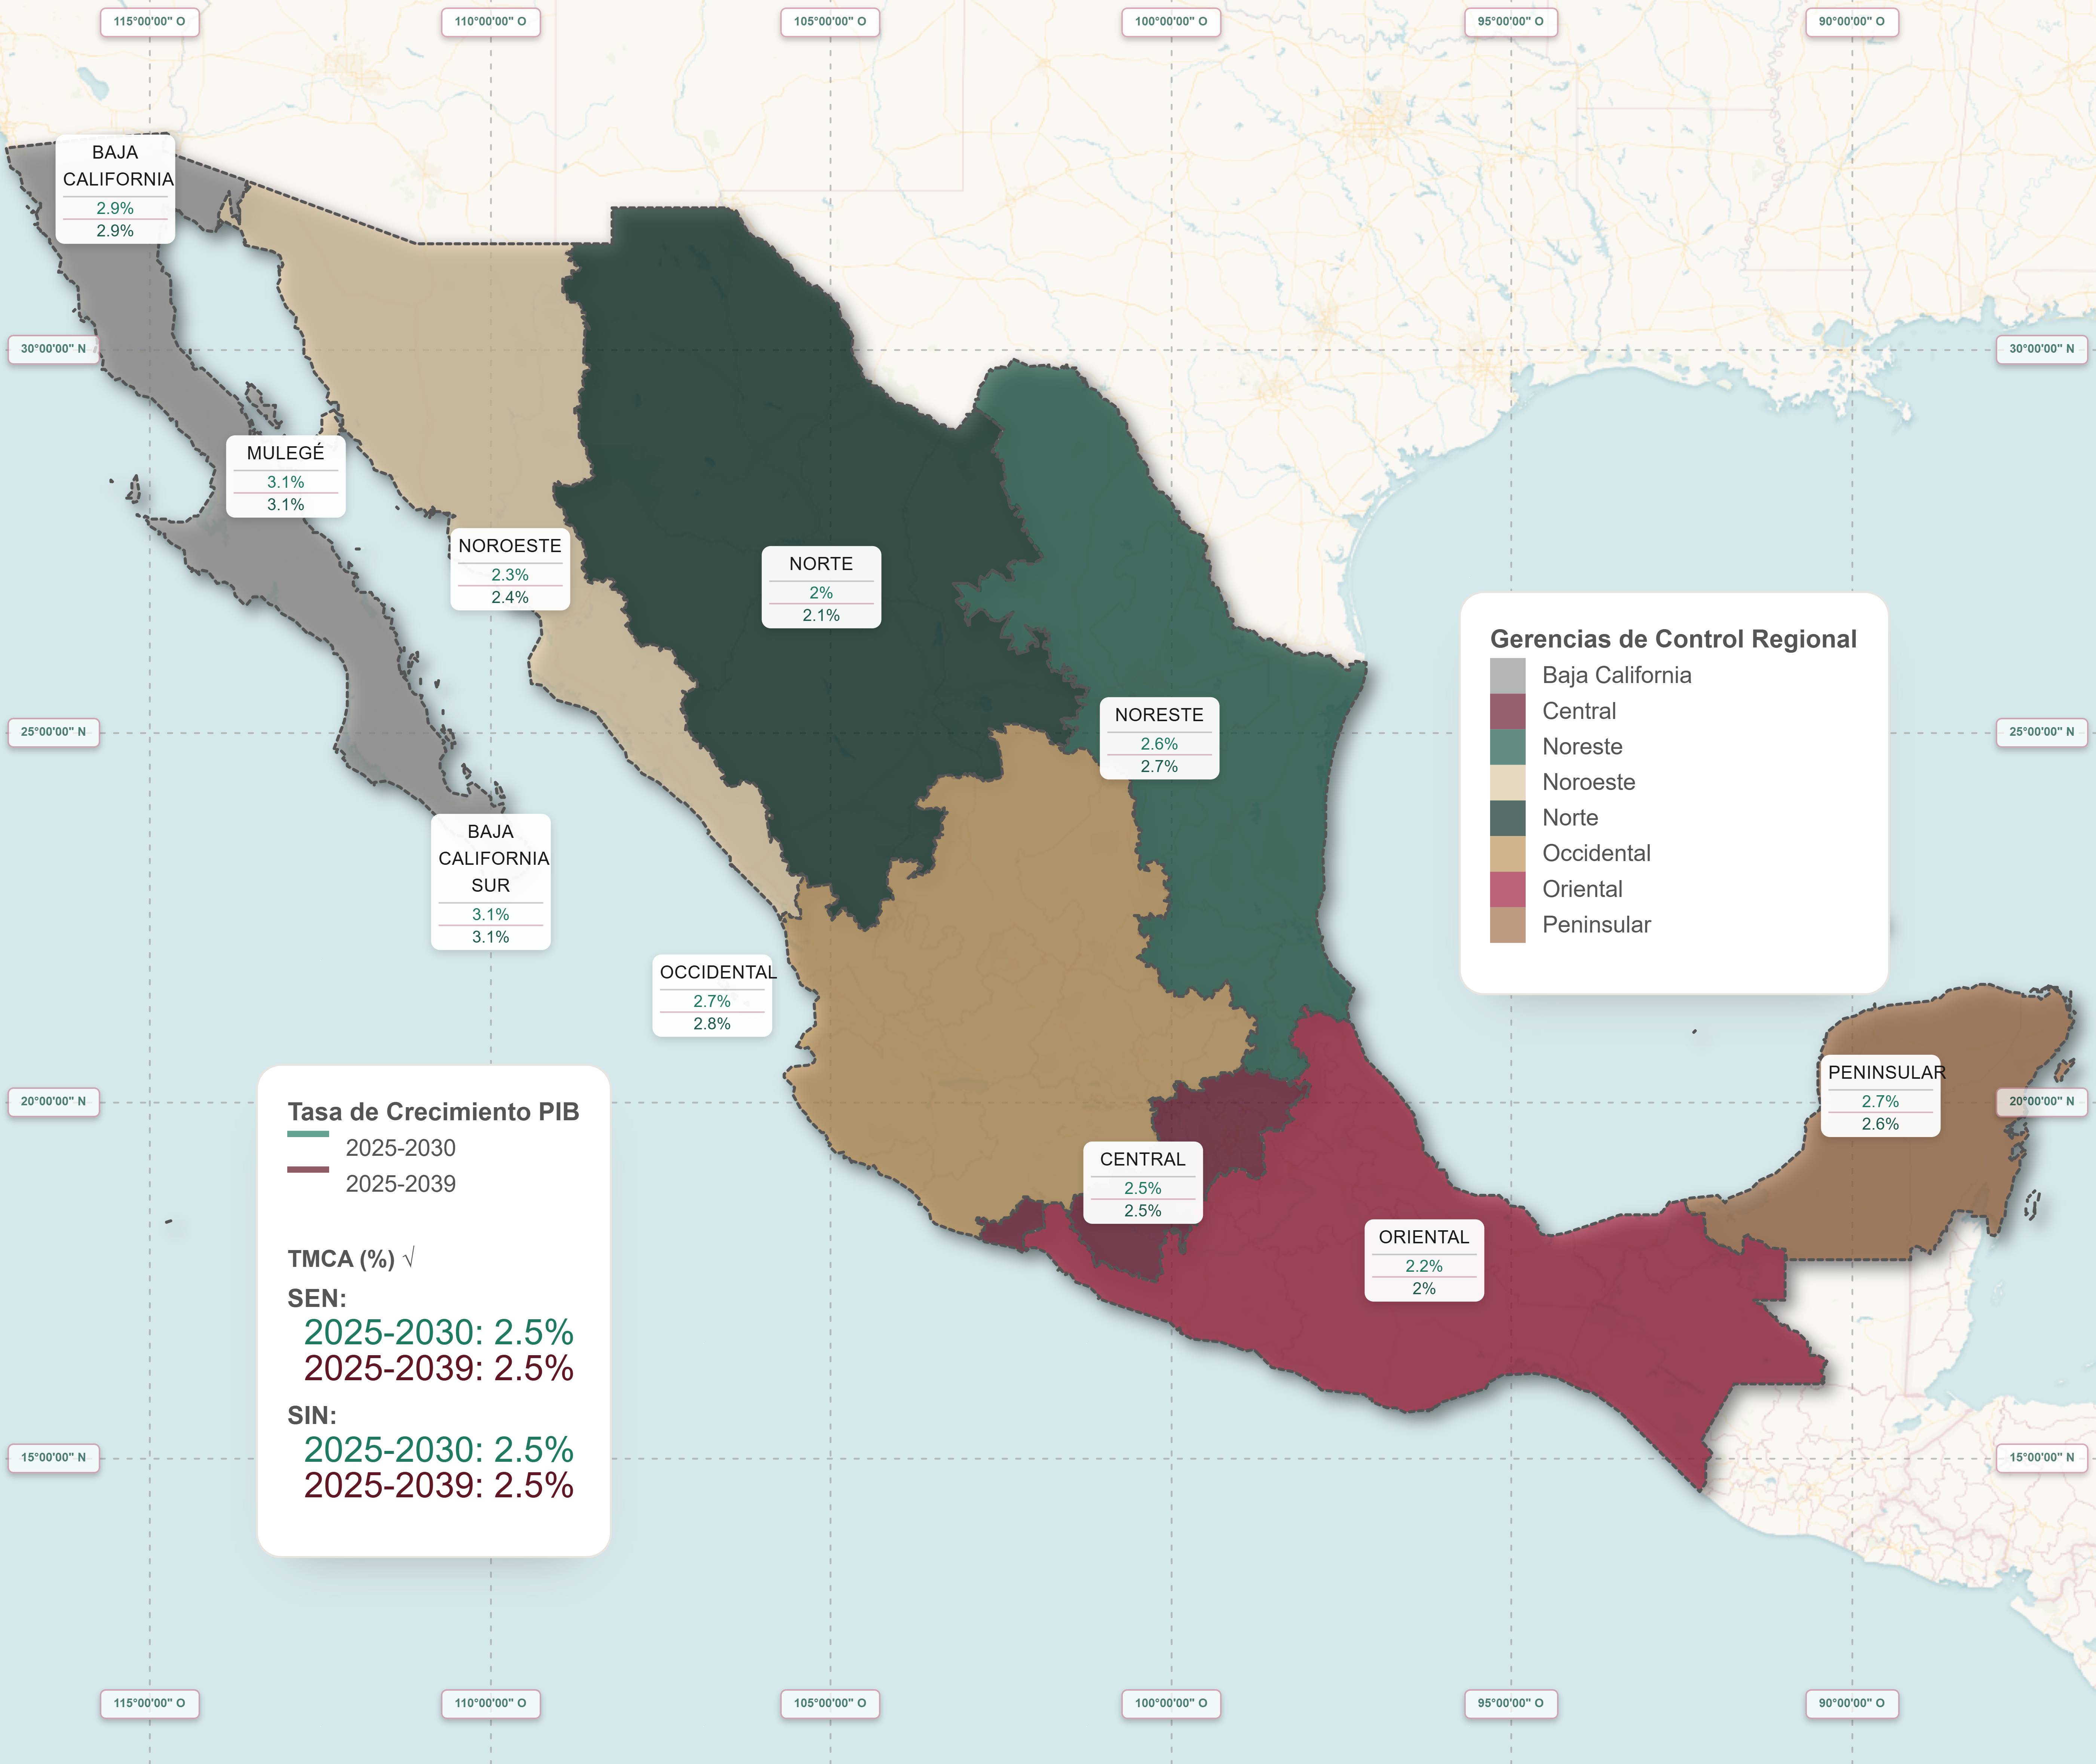
\includegraphics[width=1.0\textwidth]{img/figura_3_5.png}}{Figura 3.5 Estructura porcentual de la oferta total de energía por energético, 2024
}
  \par}
  \raggedright
  \caption{Figura 3.5 Estructura porcentual de la oferta total de energía por energético, 2024
}
  \label{fig:FIG-3.4-1}
\end{figure}
\vspace{-4pt}
\fuente{Elaboración SENER. \footnote{Otros energéticos se compone por energía nuclear, energía hidráulica, energía geotérmica, energía solar, energía eólica, bagazo de caña, leña, biogás, coque de carbón, coque de petróleo, GLP, querosenos, combustóleo, lubricantes, parafinas,asfalto, azufre, materia primanegro de humo, gasóleo, etano, gas de alto horno, gas de coque, licor negro, gas residual y aceite residual, energía eléctrica y carbón mineral.}}


La relevancia de los hidrocarburos y sus productos derivados en la oferta total de energía en México es semejante a la oferta actual e histórica de energía mundial (IEA, 2025). Contrastando el caso específico del carbón mineral, cuya participación en la oferta energética de México es marginal, mientras que a nivel mundial es el segundo energético más importante para la generación de energía eléctrica.


\subsection{Energía no aprovechada}

La energía no aprovechada (ENA), se refiere a la energía que, por disponibilidad técnica o económica durante su explotación, no se utiliza. En 2024, la ENA presentó un decrecimiento de 128.1 PJ con respecto a 2023, llegando a 261 PJ, de los cuales el gas natural y el petróleo crudo representaron casi su totalidad, con 206 PJ y 54 PJ, respectivamente, como se observa en la Figura 3.6.

\Needspace{18\baselineskip}
\begin{figure}[H]
  {\centering
  % Texto alternativo para accesibilidad
  \pdftooltip{\includegraphics[width=1.0\textwidth]{img/figura_3_6.png}}{Figura 3.6 Evolución histórica de la energía no aprovechada por energético, 2010-2024
}
  \par}
  \raggedright
  \caption{Figura 3.6 Evolución histórica de la energía no aprovechada por energético, 2010-2024
}
  \label{fig:FIG-3.5-1}
\end{figure}
\vspace{-4pt}
\fuente{Elaboración SENER.}


Durante el 2024, la ENA representó el 3.5\% de la producción nacional de energía. Considerando que el gas natural es el de mayor participación en la ENA, sigue siendo un tema prioritario aumentar su aprovechamiento, debido a que es el combustible más importado en México, según el saldo neto de la balanza comercial energética. Por ello, algunas líneas de acción del PND y PROSENER 2025-2030 se enfocan en la mejora de la eficiencia energética y el fortalecimiento de las capacidades de producción de las empresas públicas del Estado, a través de la reducción de la quema y venteo de gas natural.


\subsection{Oferta interna bruta}

La oferta interna bruta de energía es la oferta total de energía (producción, importaciones y variación de inventarios), menos las exportaciones y la ENA, es decir, representa la energía disponible en el país. En 2024, la oferta interna bruta para México fue de 9,641.77 PJ (Ver Figura 3.7), de los cuales el 76.3\% fue producción nacional, cabe señalar que esta proporción está relacionada con el grado de autosuficiencia energética que tiene el país, es decir, la capacidad para satisfacer sus necesidades energéticas con sus propios recursos.

\Needspace{18\baselineskip}
\begin{figure}[H]
  {\centering
  % Texto alternativo para accesibilidad
  \pdftooltip{\includegraphics[width=1.0\textwidth]{img/figura_3_7.png}}{Figura 3.7 Composición de la oferta interna bruta por proceso, 2024}
  \par}
  \raggedright
  \caption{Figura 3.7 Composición de la oferta interna bruta por proceso, 2024}
  \label{fig:FIG-3.6-1}
\end{figure}
\vspace{-4pt}
\fuente{Elaboración SENER.}



\portadaseccion{4}{Transformaciones, Consumo Propio y Pérdidas}{}

\section{Transformaciones, Consumo Propio y Pérdidas}

En este capítulo se evalúan los principales flujos del sector energético mexicano (SEM), la energía enviada a centros de transformación, los energéticos producidos, así como los consumos en procesos del SEM y las pérdidas que se producen en el transporte y la distribución de energía.

La transformación se refiere al proceso mediante el cual un energético es sometido a modificaciones físicas, químicas o bioquímicas, con el fin de convertirlo en un energético, genéricamente denominado como secundario, el cual es aprovechable por los usuarios intermedios o finales. Por ejemplo, los procesos en refinerías, donde energéticos primarios, como el petróleo crudo y condensados, son tratados para obtener petrolíferos, los cuales son productos energéticos con características específicas que permiten su uso en los distintos sectores de consumo. Asimismo, las centrales eléctricas, que utilizan diversos energéticos primarios como energía solar, eólica o hidráulica, o energéticos como diésel y gas seco para la generación de energía eléctrica que se utiliza en viviendas o sectores productivos.


\subsection{Refinación}

La refinación constituye una de las principales formas de transformación de hidrocarburos, principalmente petróleo crudo, hacia productos petrolíferos de consumo tanto para usuarios finales como de consumo intermedio. En 2024, estos centros de transformación emplearon 2,119.48 PJ, de los cuales 1,793.27 PJ (84.6\%) corresponden a petróleo crudo y 326.21 PJ (15.4\%) a condensados.

La Figura 4.1 muestra los productos de refinerías y despuntadoras en 2024, como se puede observar, de un total de 2,107.65PJ, los combustibles con mayor producción fueron: gas seco con 28\% (590.63 PJ), seguido del combustóleo con 27.3\% (574.97 PJ), las gasolinas y naftas con un 20.9\% (441.01PJ), y diesel con 16.3\% (344.46 PJ). El restante 7.4\% (156.58 PJ) se conformó por querosenos, otros energéticos, coque de petróleo y GLP.

\Needspace{18\baselineskip}
\begin{figure}[H]
  {\centering
  % Texto alternativo para accesibilidad
  \pdftooltip{\includegraphics[width=1.0\textwidth]{img/figura_4_1.png}}{Figura 4.1 Composición de la transformación en refinerías y despuntadoras por energético, 2024}
  \par}
  \raggedright
  \caption{Figura 4.1 Composición de la transformación en refinerías y despuntadoras por energético, 2024}
  \label{fig:FIG-4.1-1}
\end{figure}
\vspace{-4pt}
\fuente{Elaboración SENER.\footnote{Otros energéticos se compone por lubricantes, parafinas, asfaltos, materia prima negro humo, gasóleo, etano, gas de alto horno, gas de coque, licor negro, gas residual, aceite residual.}}


Cabe señalar que la transformación en refinerías ha mostrado un comportamiento irregular en los últimos quince años, como se observa en la Figura 4.2. Las fluctuaciones en la producción de estos centros de transformación reflejan el impacto de los cambios de política y de factores externos. Después de alcanzar su valor más alto en 2013, siguió un periodo de declive hasta que, en 2018, se estabilizó (aunque volvería a caer en 2020 por efectos de la pandemia de COVID19), y comenzó otro período de crecimiento entre 2021 y 2024.

\Needspace{18\baselineskip}
\begin{figure}[H]
  {\centering
  % Texto alternativo para accesibilidad
  \pdftooltip{\includegraphics[width=1.0\textwidth]{img/figura_4_2.png}}{Figura 4.2 Evolución de producción de energía en refinerías y despuntadoras por energético, 2010-2024}
  \par}
  \raggedright
  \caption{Figura 4.2 Evolución de producción de energía en refinerías y despuntadoras por energético, 2010-2024}
  \label{fig:FIG-4.1-2}
\end{figure}
\vspace{-4pt}
\fuente{Elaboración SENER.\footnote{En el periodo del 2011-2014, condensados se contabilizan en otros energéticos.}}


Es por ello que la disminución en la producción de energía de refinerías y despuntadoras en el periodo 2014-2018 se puede atribuir a las diversas reformas y programas de modernización de ese sector, las cuales no alcanzaron los resultados esperados. Esta caída también está vinculada con el descenso en la producción del petróleo crudo, que es la principal materia prima procesada en dichas instalaciones.

Sin embargo, también se observa un incremento en la producción de refinerías y despuntadoras durante el periodo 2018 y 2024, debido a las acciones y programas de rehabilitación de las 5 refinerías existentes de PEMEX (Salamanca, Minatitlán, Ciudad Madero, Cadereyta, Salina Cruz y Tula); de la adquisición de la Refinería Deer Park, y de la construcción de la nueva refinería Olmeca, en Dos Bocas, Tabasco.


\subsection{Procesamiento de gas}

En los últimos años, la transformación en plantas de gas y fraccionadoras ha seguido el comportamiento observado en refinerías y despuntadoras. El gas seco ha sido el energético más producido en este tipo de centros de transformación; sin embargo, disminuyó de forma considerable y constante durante el periodo 2013-2020 (Figura 4.3.).

\Needspace{18\baselineskip}
\begin{figure}[H]
  {\centering
  % Texto alternativo para accesibilidad
  \pdftooltip{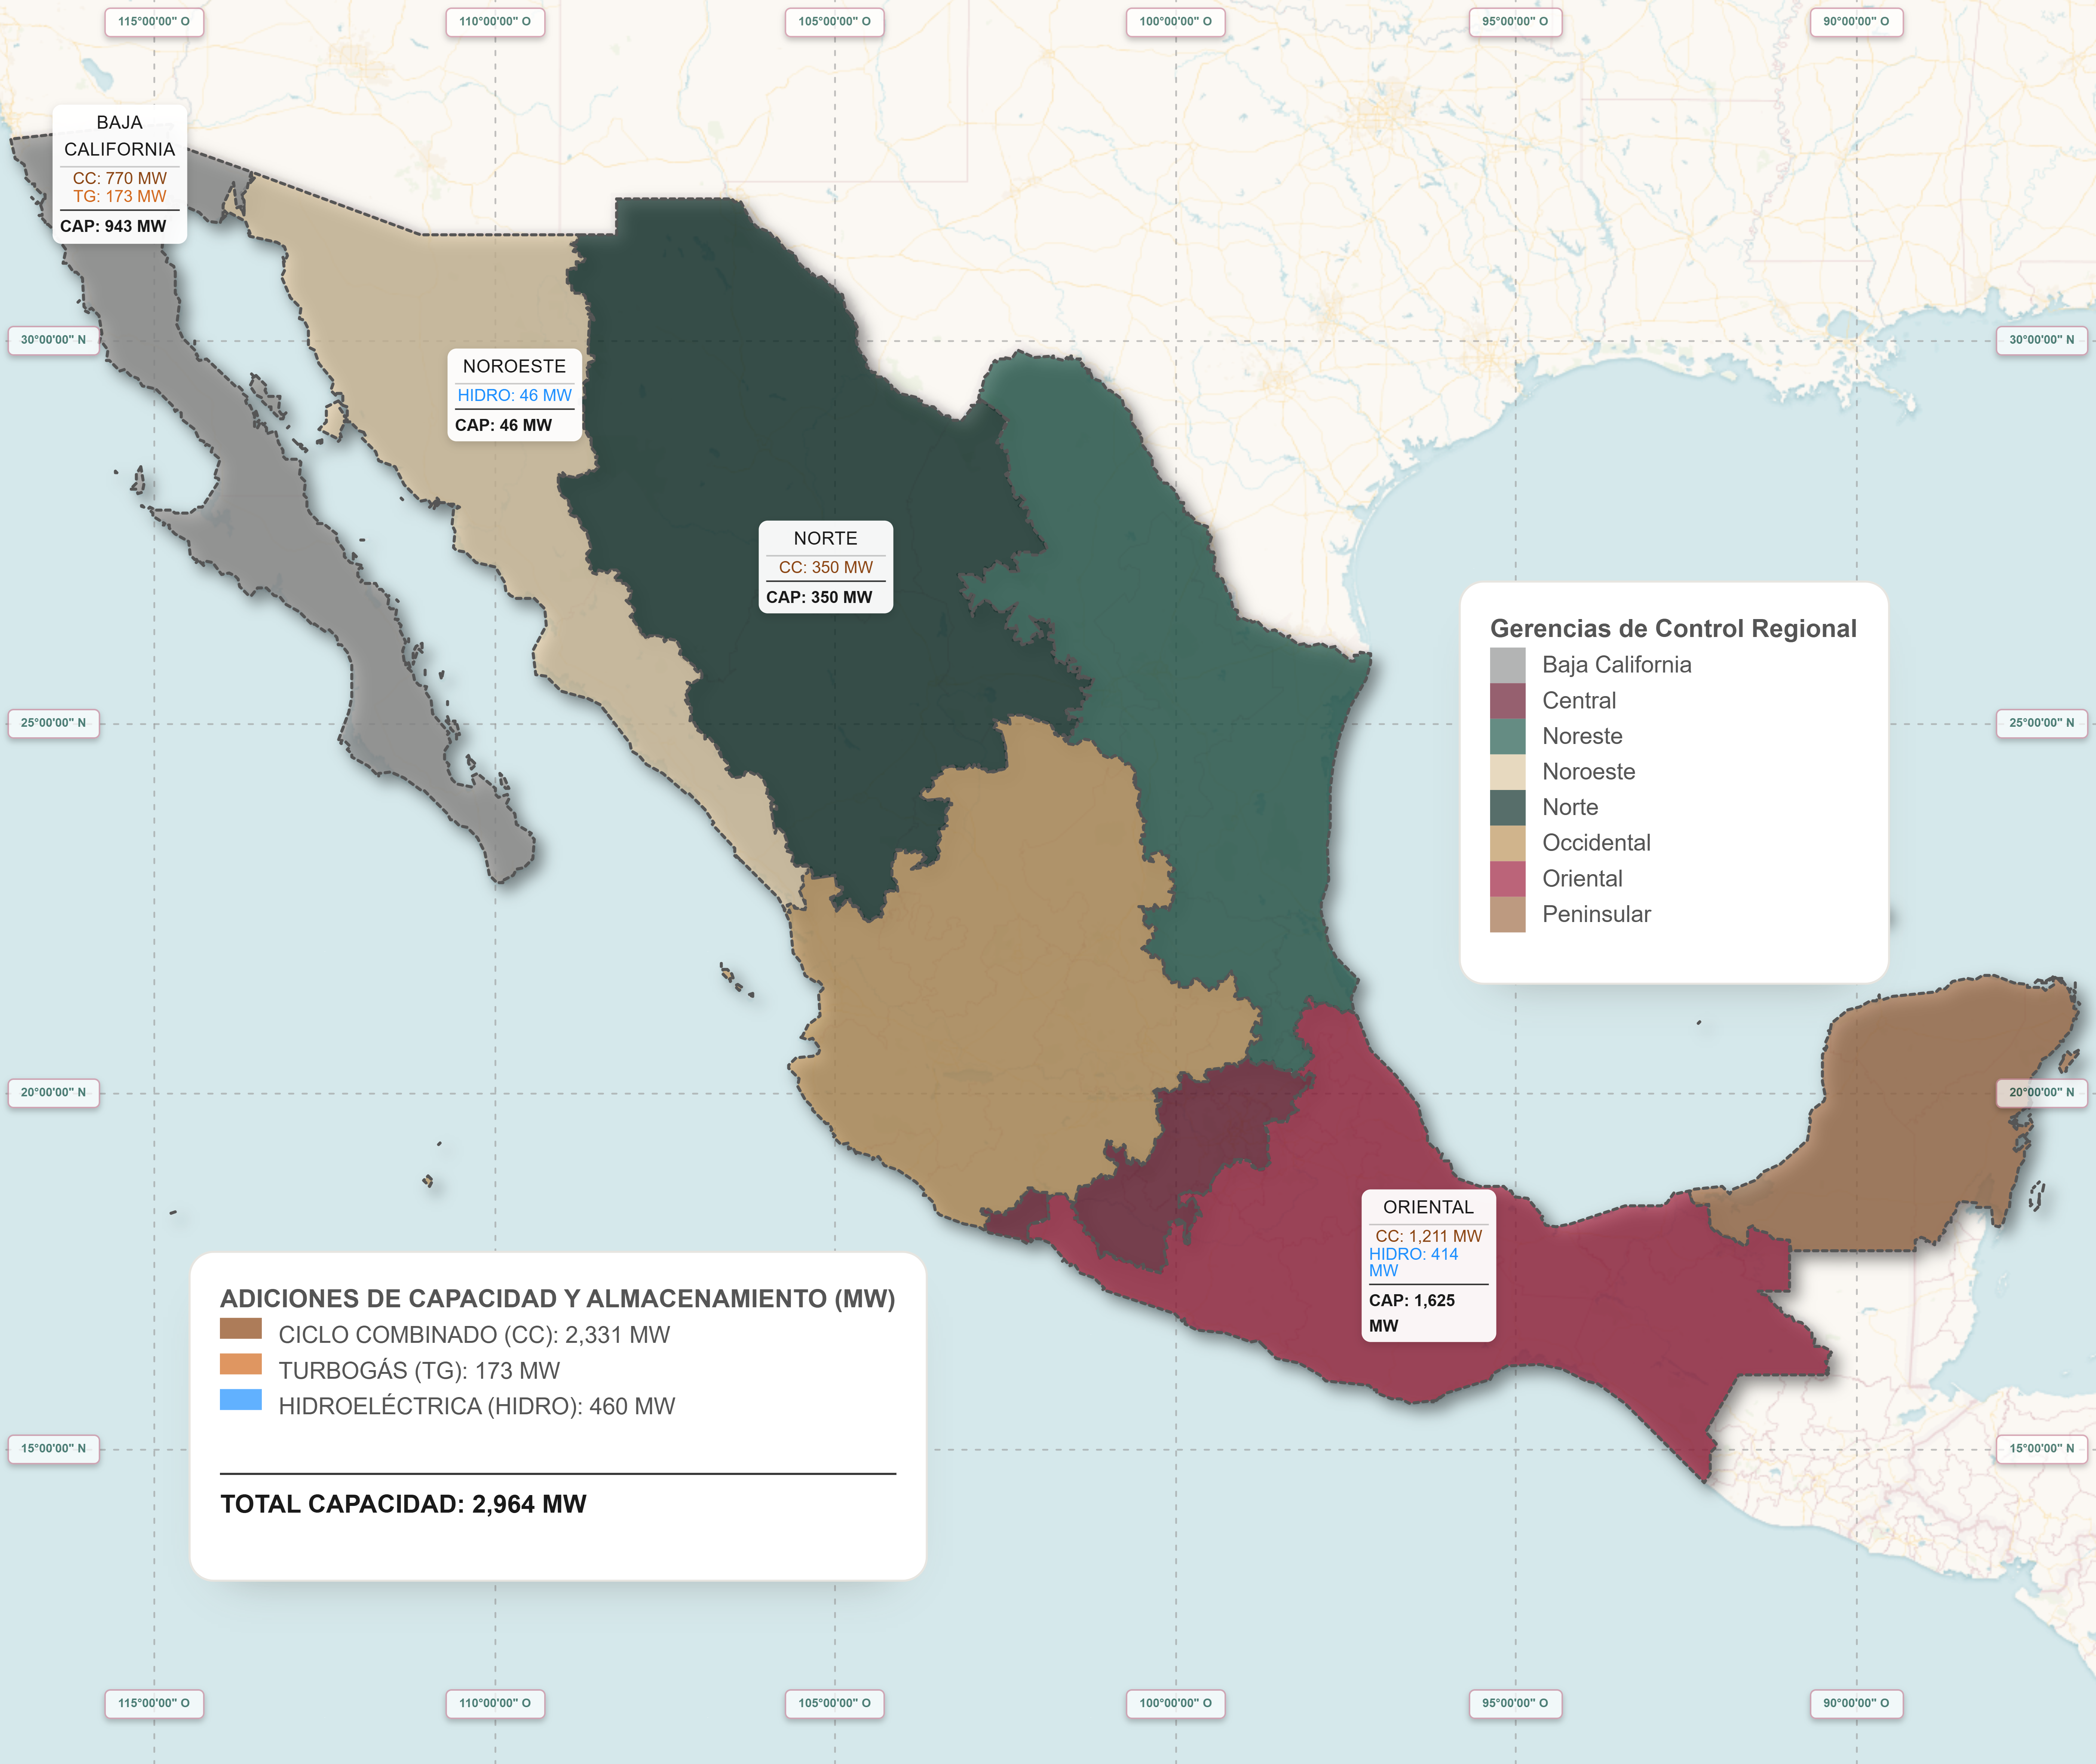
\includegraphics[width=1.0\textwidth]{img/figura_4_3.png}}{Figura 4.3 Evolución de producción de energía en plantas de gas y fraccionadoras por energético, 2010-2024
}
  \par}
  \raggedright
  \caption{Figura 4.3 Evolución de producción de energía en plantas de gas y fraccionadoras por energético, 2010-2024
}
  \label{fig:FIG-4.2-1}
\end{figure}
\vspace{-4pt}
\fuente{Elaboración SENER.}


La producción de energía en plantas de gas y fraccionadoras depende directamente de la disponibilidad de gas natural como insumo principal. Sin embargo, en los últimos años la producción de este energético (Figura 3.2.) ha mostrado una tendencia a la baja, situación que se ha visto agravada por los efectos de políticas orientadas a la importación más que a la producción de industrias asociadas como es la industria petroquímica nacional.

Sin embargo, a partir de 2020, la producción en plantas de gas y fraccionadoras ha incrementado la disponibilidad de GLP así como de gasolinas y naftas. De manera similar, la implementación de políticas, como parte del rescate a PEMEX, han contribuido a garantizar el abastecimiento a los centros de transformación para producir gas seco. En 2024, las plantas de gas y fraccionadoras utilizaron como insumo 1,364.56 PJ, de los cuales 1,052.40 PJ (77.1\%) corresponden a gas natural y 312.16 PJ (22.9\%) a condensados. Estos centros de transformación, produjeron 908 PJ de los cuales 634.10 PJ (69.8\%) corresponden a gas seco; 150.37 PJ (16.6\%) a GLP; 73.63 PJ (8.1\%) a gasolinas y naftas y finalmente 50.03 PJ (5.5\%) a otros energéticos (Figura 4.4).

\Needspace{18\baselineskip}
\begin{figure}[H]
  {\centering
  % Texto alternativo para accesibilidad
  \pdftooltip{\includegraphics[width=1.0\textwidth]{img/figura_4_4.png}}{Figura 4.4 Composición de la producción de energía en plantas de gas y fraccionadoras, 2024
}
  \par}
  \raggedright
  \caption{Figura 4.4 Composición de la producción de energía en plantas de gas y fraccionadoras, 2024
}
  \label{fig:FIG-4.2-2}
\end{figure}
\vspace{-4pt}
\fuente{Elaboración SENER.}



\subsection{Generación eléctrica}

La energía eléctrica resulta de la transformación en centrales eléctricas de fuentes primarias de energía (hidrocarburos, energía nuclear, potencial hidráulico, energía solar, energía eólica, energía geotérmica, entre otras), así como de energéticos secundarios (gas seco, combustóleo, diésel, entre otros). En el país, estos centros de transformación generaron 1,381.52 PJ (383,754 GWh) de energía eléctrica durante 2024. Para ello, se requirieron 3,405.56 PJ de insumos energéticos, lo que se traduce en una eficiencia global del sistema cercana al 40.6\%.

La matriz de insumos energéticos para la generación de energía eléctrica en 2024 estuvo dominada por el gas seco, con el 64.2\% (2,186.18 PJ), seguido de fuentes de energía renovable con el 24.8\% (844.12 PJ), de los cuales la energía hidráulica representó el 7.7\% (262.18 PJ), la energía eólica el 6.5\% (220.18 PJ), la energía solar con el 6\% (205.70 PJ), la geoenergía con el 2.7\% (91.32 PJ), el bagazo de caña con el 1.8\% (61.5 PJ) y el biogás con apenas el 0.1\% (3.25 PJ). En tanto que otros energéticos como el carbón mineral contribuyó con el 4.3\% (147.47 PJ), la energía nuclear con el 3.8\% (129.51 PJ), el combustóleo con el 1.4\% (47.09 PJ), el diésel con el 1\% (33.43 PJ) y el coque de petróleo con apenas el 0.5\% (17.77 PJ) (Figura 4.5.).

\Needspace{18\baselineskip}
\begin{figure}[H]
  {\centering
  % Texto alternativo para accesibilidad
  \pdftooltip{\includegraphics[width=1.0\textwidth]{img/figura_4_5.png}}{Figura 4.5 Energéticos empleados para la generación de energía eléctrica, 2024}
  \par}
  \raggedright
  \caption{Figura 4.5 Energéticos empleados para la generación de energía eléctrica, 2024}
  \label{fig:FIG-4.3-1}
\end{figure}
\vspace{-4pt}
\fuente{Elaboración SENER.}


En cuanto a las tecnologías utilizadas para la generación de energía eléctrica, destaca el crecimiento en la participación de las centrales de ciclo combinado que, como se observa en la Figura 4.6, aportaron el 58\% de la generación bruta de energía eléctrica en 2024, al tiempo que ha disminuido la participación de las centrales carboeléctricas y termoeléctricas convencionales en los últimos años, en alineación con una estrategia de descarbonización progresiva y con la necesidad de responder a una demanda eléctrica en constante crecimiento.

\Needspace{18\baselineskip}
\begin{figure}[H]
  {\centering
  % Texto alternativo para accesibilidad
  \pdftooltip{\includegraphics[width=1.0\textwidth]{img/figura_4_6.png}}{Figura 4.6 Evolución de la generación bruta de energía eléctrica por tecnología, 2010-2024
}
  \par}
  \raggedright
  \caption{Figura 4.6 Evolución de la generación bruta de energía eléctrica por tecnología, 2010-2024
}
  \label{fig:FIG-4.3-2}
\end{figure}
\vspace{-4pt}
\fuente{Elaboración SENER.}



\subsection{Consumo propio del sector}

El consumo propio del sector energético se refiere a la energía primaria y secundaria utilizada para el funcionamiento interno de instalaciones; es decir, en la operación de pozos, refinerías, centrales de generación eléctrica, entre otros.

Como se muestra en la Figura 4.7, en el periodo 2010-2024, el consumo propio del sector ha disminuido, presentando un comportamiento acoplado a la tendencia a la baja de la producción de energía en el país. La predominancia del gas seco se ha mantenido a lo largo de los últimos 15 años (Figura 4.7), con un pico notable en 2020. Esta situación afecta negativamente el avance hacia la autosuficiencia, la soberanía y la seguridad energética del país, dado que el gas seco es el principal energético que se importa en México.

\Needspace{18\baselineskip}
\begin{figure}[H]
  {\centering
  % Texto alternativo para accesibilidad
  \pdftooltip{\includegraphics[width=1.0\textwidth]{img/figura_4_7.png}}{Figura 4.7 Evolución del consumo propio del sector por energético, 2010 - 2024
}
  \par}
  \raggedright
  \caption{Figura 4.7 Evolución del consumo propio del sector por energético, 2010 - 2024
}
  \label{fig:FIG-4.4-1}
\end{figure}
\vspace{-4pt}
\fuente{Elaboración SENER.}


En 2024, el total de energía consumida por el sector energético fue de 1,608.7 PJ. El energético de mayor consumo en los procesos e instalaciones del sector fue el gas seco, que representó el 53.4\% (859.49 PJ), seguido por el gas natural con 37\% (595.69 PJ), cubriendo más del 90\% entre ambos energéticos (Ver Figura 4.8.). El restante 9.5\% en el consumo propio del sector está conformado por energía eléctrica con 4.2\% (67.89 PJ), otros energéticos con 1.4\% (23.04 PJ), combustóleo con 0.7\% (11.25 PJ), coque de petróleo con 0.5\% (7.83 PJ), gasolinas y naftas con 0.3\% (4.15 PJ), GLP con 0.2\% (2.66 PJ) y coque de carbón con 0.02\% (0.36 PJ).

\Needspace{18\baselineskip}
\begin{figure}[H]
  {\centering
  % Texto alternativo para accesibilidad
  \pdftooltip{\includegraphics[width=1.0\textwidth]{img/figura_4_8.png}}{Figura 4.8 Estructura porcentual del consumo propio del sector por energético, 2024
}
  \par}
  \raggedright
  \caption{Figura 4.8 Estructura porcentual del consumo propio del sector por energético, 2024
}
  \label{fig:FIG-4.4-2}
\end{figure}
\vspace{-4pt}
\fuente{Elaboración SENER.}



\subsection{Pérdidas}

Las pérdidas de energía por transporte, transmisión y distribución por energético son las mermas de energía que ocurren a lo largo de la cadena de suministro, desde la producción hasta el consumo final. Estas pérdidas se originan por factores físicos inherentes al transporte, transmisión o distribución de los energéticos, como fricción, disipación térmica, fugas o resistencia eléctrica. Conviene destacar que en los petrolíferos, estas pérdidas suelen integrarse dentro del consumo propio del sector energético.

En el caso de la energía eléctrica, se clasifican en dos tipos: pérdidas técnicas y pérdidas no técnicas. Por un lado, las pérdidas técnicas se producen de forma inevitable durante el proceso de transmisión y distribución de la electricidad. Estas pérdidas se manifiestan principalmente como energía térmica generada por el calentamiento de los conductores, transformadores y demás componentes de la infraestructura de transporte de electricidad en el SEN, cuando la corriente eléctrica circula a través de ellos. Este fenómeno se conoce como el efecto Joule, y es una consecuencia directa de la resistencia eléctrica de los materiales. Las pérdidas técnicas forman parte del funcionamiento normal de un sistema eléctrico.

Por otro lado, se denominan pérdidas no técnicas cuando parte del consumo no se registra en los sistemas de medición. Estas pérdidas no están relacionadas con las propiedades físicas del sistema, sino que se originan por causas como el uso ilícito de la energía, fallas o manipulaciones en los equipos de medición, errores administrativos, omisiones en el registro de datos, facturación incorrecta, entre otras causas.

En el periodo 2010-2024, las pérdidas energéticas presentaron una tendencia decreciente a lo largo del periodo (TMDA de 0.9\%), principalmente por la reducción de pérdidas técnicas, alcanzando un mínimo en 2019 (147.28 PJ). A partir de ese año, las pérdidas han experimentado un crecimiento, mayormente provocado por el incremento de las pérdidas no técnicas. En 2024, las pérdidas alcanzaron un valor de 168.01 PJ, 5.03\% mayor que en 2023 (Figura 4.9).

\Needspace{18\baselineskip}
\begin{figure}[H]
  {\centering
  % Texto alternativo para accesibilidad
  \pdftooltip{\includegraphics[width=1.0\textwidth]{img/figura_4_9.png}}{Figura 4.9 Evolución de las pérdidas energéticas, 2010-2024
}
  \par}
  \raggedright
  \caption{Figura 4.9 Evolución de las pérdidas energéticas, 2010-2024
}
  \label{fig:FIG-4.5-1}
\end{figure}
\vspace{-4pt}
\fuente{Elaboración SENER.}


Como se mencionó con anterioridad, las pérdidas energéticas en 2024 fueron de 168.01 PJ, de las cuales 102.88 PJ (61.23\%) son pérdidas técnicas y 65.13 PJ (38.77\%) son pérdidas no técnicas (Figura 4.10.).

\Needspace{18\baselineskip}
\begin{figure}[H]
  {\centering
  % Texto alternativo para accesibilidad
  \pdftooltip{\includegraphics[width=1.0\textwidth]{img/figura_4_10.png}}{Figura 4.10 Estructura porcentual de las pérdidas energéticas, 2024
}
  \par}
  \raggedright
  \caption{Figura 4.10 Estructura porcentual de las pérdidas energéticas, 2024
}
  \label{fig:FIG-4.5-2}
\end{figure}
\vspace{-4pt}
\fuente{Elaboración SENER.}



\portadaseccion{5}{Consumo final}{}

\section{Consumo final}

La energía disponible en el país llega a los usuarios finales para su aprovechamiento en diversas actividades, tanto económicas, como de la vida cotidiana. Con el objetivo de describir el consumo final en el país durante el periodo 2010-2024, con énfasis en 2024, este capítulo desglosa los patrones de consumo energético en los seis principales sectores de consumo en el país: agropecuario, industrial, comercial y servicios, residencial, público y transporte, así como del consumo no energético, el cual representa el uso de energéticos en la elaboración de productos como plásticos, fertilizantes, solventes, entre otros.

La Figura 5.1. muestra la participación de cada sector en el consumo final para 2024, evidenciando que el sector transporte es el de mayor participación, con el 44\% del consumo energético final; seguido del industrial y el residencial con 32.8\% y 12.7\%, respectivamente. En tanto que los sectores de menor participación son el comercial y servicios, así como agropecuario con 3.4\% cada uno, mientras que el sector no energético tuvo una participación del 3.3\% y finalmente el sector público es el de menor proporción con apenas del 0.5\% del consumo final.

\Needspace{18\baselineskip}
\begin{figure}[H]
  {\centering
  % Texto alternativo para accesibilidad
  \pdftooltip{\includegraphics[width=1.0\textwidth]{img/figura_5_1.png}}{Figura 5.1 Participación de los distintos sectores de consumo final, 2024
}
  \par}
  \raggedright
  \caption{Figura 5.1 Participación de los distintos sectores de consumo final, 2024
}
  \label{fig:FIG-5-1}
\end{figure}
\vspace{-4pt}
\fuente{Elaboración SENER.}


La distribución sectorial del consumo final se ha comportado de manera estable los últimos 15 años, salvo durante periodo 2019-2021, ya que la pandemia condicionó los patrones de consumo, especialmente en materia de movilidad, lo que impactó de manera significativa la disminución del consumo en el sector transporte, como se muestra en la Figura 5.2.

\Needspace{18\baselineskip}
\begin{figure}[H]
  {\centering
  % Texto alternativo para accesibilidad
  \pdftooltip{\includegraphics[width=1.0\textwidth]{img/figura_5_2.png}}{Figura 5.2 Evolución del consumo final por sector, 2010 - 2024}
  \par}
  \raggedright
  \caption{Figura 5.2 Evolución del consumo final por sector, 2010 - 2024}
  \label{fig:FIG-5-2}
\end{figure}
\vspace{-4pt}
\fuente{Elaboración SENER.}



\subsection{Sector agropecuario}

El consumo energético del sector agropecuario fue de 188.02 PJ en 2024. En la Figura 5.3 se observa que los principales energéticos consumidos fueron el diésel y la energía eléctrica (96.1\% del consumo del sector en conjunto), con 126.84 PJ (67.5\%) y 53.88 PJ (28.7\%) respectivamente. El restante se distribuye entre el GLP con 5.55 PJ (3\%), combustóleo con 1.29 PJ (0.7\%), y gas seco con 0.47 PJ (0.2\%).

La importancia del diésel en el consumo de este sector es atribuible al uso de maquinaria en el trabajo de campo (tractores, camiones de carga de cultivos y ganado, entre otros). Dada la importancia del diésel para el sector agropecuario, es importante remarcar que es uno de los energéticos secundarios de mayor déficit comercial en el país, después del gas seco y las gasolinas y naftas, como se presentó en la Figura 3.3.

Por su parte, la energía eléctrica es utilizada para sistemas de riego, drenaje, bombeo de agua, iluminación y calefacción en invernaderos, ventilación de instalaciones ganaderas, etc.

\Needspace{18\baselineskip}
\begin{figure}[H]
  {\centering
  % Texto alternativo para accesibilidad
  \pdftooltip{\includegraphics[width=1.0\textwidth]{img/figura_5_3.png}}{Figura 5.3 Composición del consumo energético del sector agropecuario por energético, 2024
}
  \par}
  \raggedright
  \caption{Figura 5.3 Composición del consumo energético del sector agropecuario por energético, 2024
}
  \label{fig:FIG-5.1-1}
\end{figure}
\vspace{-4pt}
\fuente{Elaboración SENER.}


El estado actual del consumo energético del sector agropecuario responde al comportamiento histórico, ya que de 2010 a 2024, el diésel y la energía eléctrica se mantuvieron como los energéticos más consumidos por dicho sector, según se muestra en la Figura 5.4.

\Needspace{18\baselineskip}
\begin{figure}[H]
  {\centering
  % Texto alternativo para accesibilidad
  \pdftooltip{\includegraphics[width=1.0\textwidth]{img/figura_5_4.png}}{Figura 5.4 Evolución del consumo energético del sector agropecuario por energético, 2010-2024
}
  \par}
  \raggedright
  \caption{Figura 5.4 Evolución del consumo energético del sector agropecuario por energético, 2010-2024
}
  \label{fig:FIG-5.1-2}
\end{figure}
\vspace{-4pt}
\fuente{Elaboración SENER.}


Por otro lado, en la Figura 5.5 se presentan los diferentes usos finales que tuvo el consumo energético total del sector en 2024. Se observa que la energía eléctrica se utilizó predominantemente para el bombeo de agua y el riego agrícola; mientras que el diésel se utilizó principalmente para maquinaria y equipos, así como para otros usos térmicos.

\Needspace{18\baselineskip}
\begin{figure}[H]
  {\centering
  % Texto alternativo para accesibilidad
  \pdftooltip{\includegraphics[width=1.0\textwidth]{img/figura_5_5.png}}{Figura 5.5 Estructura del consumo energético del sector agropecuario por uso final, 2024}
  \par}
  \raggedright
  \caption{Figura 5.5 Estructura del consumo energético del sector agropecuario por uso final, 2024}
  \label{fig:FIG-5.1-3}
\end{figure}
\vspace{-4pt}
\fuente{Elaboración SENER.}



\subsection{Sector industrial}

En el año 2024, el sector industrial tuvo un consumo eléctrico de 1,826.95PJ, los principales energéticos utilizados en este sector fueron la energía eléctrica y el gas seco con una participación de 38.60\% (705.12 PJ) y 38.42\% (701.91PJ), respectivamente (Figura 5.6). En tanto que la participación de otros energéticos se conformó de la siguiente manera: coque de petróleo con 7\%, carbón mineral con 3.9\%, diésel con 3.5\%, GLP con 2.9\%, bagazo de caña con 1.8\% y energía solar con 1.7\%. Finalmente, los energéticos que menor proporción tuvieron son el coque de carbón, el combustóleo, la leña y las gasolinas y naftas con 0.9\%, 0.6\%, 0.5\% y 0.1\%, respectivamente.

\Needspace{18\baselineskip}
\begin{figure}[H]
  {\centering
  % Texto alternativo para accesibilidad
  \pdftooltip{\includegraphics[width=1.0\textwidth]{img/figura_5_6.png}}{Figura 5.6 Composición del consumo de energía del sector industrial por energético, 2024
}
  \par}
  \raggedright
  \caption{Figura 5.6 Composición del consumo de energía del sector industrial por energético, 2024
}
  \label{fig:FIG-5.2-1}
\end{figure}
\vspace{-4pt}
\fuente{Elaboración SENER.}


Como se observa en la Figura 5.7, la preponderancia del consumo de energía eléctrica y el gas seco se ha mantenido en el sector industrial durante el periodo 2010-2024. Esta tendencia muestra la magnitud de la dependencia de un sector estratégico como es el industrial al gas seco, por un lado debido a que en México el gas seco es el energético que más se importa y es el más utilizado en la generación de energía eléctrica, y por el otro el consumo importante de gas seco en procesos de este sector (Figura 3.3).

\Needspace{18\baselineskip}
\begin{figure}[H]
  {\centering
  % Texto alternativo para accesibilidad
  \pdftooltip{\includegraphics[width=1.0\textwidth]{img/figura_5_7.png}}{Figura 5.7 Evolución del consumo de energía del sector industrial por energético, 2010-2024
}
  \par}
  \raggedright
  \caption{Figura 5.7 Evolución del consumo de energía del sector industrial por energético, 2010-2024
}
  \label{fig:FIG-5.2-2}
\end{figure}
\vspace{-4pt}
\fuente{Elaboración SENER.}


En la Figura 5.8, se hace un desglose más detallado de las ramas industriales con mayor consumo energético en México. Es importante señalar que la información ha sido agrupada de acuerdo a la versión actual del Sistema de Clasificación Industrial de América del Norte (SCIAN).

La mayoría de las ramas industriales tuvieron principalmente un consumo de gas seco y energía eléctrica en 2024, se estimó que cerca de la mitad requieren primordialmente de energía eléctrica (212, 213, 314, 315, 332, 333, 335, 336 y Otras actividades), mientras que el resto (311, 313, 322, 325, 326, 331 y 336) son altamente dependientes del gas seco. A su vez, se concluyó que la fabricación de productos cuya base es de minerales no metálicos (327) se tiene una menor dependencia a los dos energéticos preponderantes en el sector y consume primordialmente coque de petróleo; mientras que, de manera similar, la industria alimentaria (213) tiene un importante consumo de bagazo de caña. Finalmente, aunque sus consumos totales no son grandes (<18 PJ), las industrias relacionadas con la construcción (236, 237, 238) hacen uso primordialmente del diésel (Figura 5.8).

\Needspace{18\baselineskip}
\begin{figure}[H]
  {\centering
  % Texto alternativo para accesibilidad
  \pdftooltip{\includegraphics[width=1.0\textwidth]{img/figura_5_8.png}}{Figura 5.8 Estructura del consumo de energía en el sector industrial por uso final, 2024}
  \par}
  \raggedright
  \caption{Figura 5.8 Estructura del consumo de energía en el sector industrial por uso final, 2024}
  \label{fig:FIG-5.2-3}
\end{figure}
\vspace{-4pt}
\fuente{Elaboración SENER.\footnote{Las ramas industriales se clasifican de la siguiente manera: 212. Minería de minerales metálicos y no metálicos, excepto petróleo y gas; 213. Servicios relacionados con la minería; 236. Edificación; 237. Construcción de obras de ingeniería civil; 238. Trabajos especializados para la construcción; 311. Industria alimentaria; 312; Industria de las bebidas y del tabaco; 313. Fabricación de insumos textiles y acabado de textiles; 314. Fabricación de productos textiles, excepto prendas de vestir; 315. Fabricación de prendas de vestir; 322. Industria del papel; 325. Industria química; 326. Industria del plástico y del hule; 327. Fabricación de productos a base de minerales no metálicos; 331. Industrias metálicas básicas; 332. Fabricación de productos metálicos; 333. Fabricación de maquinaria y equipo; 334. Fabricación de equipo de computación, comunicación, medición y de otros equipos, componentes y accesorios electrónicos; 335. Fabricación de accesorios, aparatos eléctricos y equipo de generación de energía eléctrica; 336, Fabricación de equipo de transporte, y Otras actividades.}}


El panorama revela una fuerte conexión entre el incremento y recuperación de la producción de gas nacional y el desarrollo del sector industrial. En estas condiciones, cobra mayor importancia el fortalecimiento de la capacidad productiva y operativa de la CFE (sustituyendo el gas seco en la generación eléctrica por energéticos de fuentes renovables), así como el incremento de la producción nacional de gas de PEMEX, acorde a los objetivos, estrategias y líneas de acción del PND y del PROSENER 2025-2030.


\subsection{Sector comercial y servicios}

En 2024, el sector comercial y servicios tuvo un consumo total 187.80 PJ. La Figura 5.9 muestra que el GLP y la energía eléctrica fueron los energéticos con la mayor participación en el consumo energético del sector, con 82.07 PJ (43.7\%) y 78.65 (41.9\%) PJ, respectivamente. Otros energéticos utilizados en el sector tuvieron una participación menor tales como el gas seco con 9.6\%, leña con 2.5\% y energía solar con 2.3\%; este comportamiento se ha mantenido durante el periodo 2010-2024, destacando su acelerado crecimiento a partir de 2020 (Figura 5.10).

\Needspace{18\baselineskip}
\begin{figure}[H]
  {\centering
  % Texto alternativo para accesibilidad
  \pdftooltip{\includegraphics[width=1.0\textwidth]{img/figura_5_9.png}}{Figura 5.9 Composición del consumo energético del sector comercial y servicios por energético, 2024
}
  \par}
  \raggedright
  \caption{Figura 5.9 Composición del consumo energético del sector comercial y servicios por energético, 2024
}
  \label{fig:FIG-5.3-1}
\end{figure}
\vspace{-4pt}
\fuente{Elaboración SENER.}


\Needspace{18\baselineskip}
\begin{figure}[H]
  {\centering
  % Texto alternativo para accesibilidad
  \pdftooltip{\includegraphics[width=1.0\textwidth]{img/figura_5_10.png}}{Figura 5.10 Evolución del consumo de energía del sector comercial y servicios por energético, 2010-2024
}
  \par}
  \raggedright
  \caption{Figura 5.10 Evolución del consumo de energía del sector comercial y servicios por energético, 2010-2024
}
  \label{fig:FIG-5.3-2}
\end{figure}
\vspace{-4pt}
\fuente{Elaboración SENER.}


Es de notar que la relevancia de la energía eléctrica se atribuye a usos finales de iluminación, climatización, refrigeración y otros usos en las diversas unidades económicas del sector. Mientras que el consumo de GLP se asocia a la cocción de los alimentos y el calentamiento de agua; sin embargo, como se observa en la Figura 5.11., la energía solar, la leña y el gas seco son importantes, principalmente, en los usos térmicos como son el calentamiento de agua y la cocción de alimentos.

\Needspace{18\baselineskip}
\begin{figure}[H]
  {\centering
  % Texto alternativo para accesibilidad
  \pdftooltip{\includegraphics[width=1.0\textwidth]{img/figura_5_11.png}}{Figura 5.11 Estructura del consumo de energía del sector comercial y servicios por uso final, 2024
}
  \par}
  \raggedright
  \caption{Figura 5.11 Estructura del consumo de energía del sector comercial y servicios por uso final, 2024
}
  \label{fig:FIG-5.3-3}
\end{figure}
\vspace{-4pt}
\fuente{Elaboración SENER.}



\subsection{Sector residencial}

Se estima que en 2024, el consumo energético de las personas que habitan en las aproximadamente 38 millones de viviendas en el país (INEGI, 2024) fue de 704.29 PJ. En la Figura 5.12. se muestra que la energía eléctrica fue el energético más consumido, con 281.23 PJ (39.9\%); seguido del GLP con 268.09 PJ (38.1\%); y la leña con 114.93 PJ\footnote{El consumo de leña se estimó a partir de la metodología establecida en Pérez et al. 2022 y los consumos por tipo de usuario exclusivo y mixto encontrados en la ENCEVI (Encuesta Nacional de Consumo de Energéticos en Viviendas Particulares) (INEGI, 2018).} (16.3\%).

\Needspace{18\baselineskip}
\begin{figure}[H]
  {\centering
  % Texto alternativo para accesibilidad
  \pdftooltip{\includegraphics[width=1.0\textwidth]{img/figura_5_12.png}}{Figura 5.12 Composición del consumo de energía del sector residencial por energético, 2024
}
  \par}
  \raggedright
  \caption{Figura 5.12 Composición del consumo de energía del sector residencial por energético, 2024
}
  \label{fig:FIG-5.4-1}
\end{figure}
\vspace{-4pt}
\fuente{Elaboración SENER.}


La energía eléctrica, el GLP y la leña han permanecido como los energéticos de mayor consumo en viviendas, como se muestra en la Figura 5.13; no obstante, destaca el crecimiento de la participación de la energía solar que, a pesar de representar menos del 2\% en el consumo de energía de este sector para 2024, ha aumentado cerca de tres veces su proporción en los últimos 15 años. De manera similar, la energía eléctrica ha adquirido una mayor presencia, debido a su uso generalizado para satisfacer las necesidades básicas y de la vida diaria de la población en las viviendas del país.

\Needspace{18\baselineskip}
\begin{figure}[H]
  {\centering
  % Texto alternativo para accesibilidad
  \pdftooltip{\includegraphics[width=1.0\textwidth]{img/figura_5_13.png}}{Figura 5.13 Evolución del consumo de energía del sector residencial por energético, 2010-2024
}
  \par}
  \raggedright
  \caption{Figura 5.13 Evolución del consumo de energía del sector residencial por energético, 2010-2024
}
  \label{fig:FIG-5.4-2}
\end{figure}
\vspace{-4pt}
\fuente{Elaboración SENER.}


El consumo de energía eléctrica en el sector residencial está relacionado con la iluminación, climatización y al uso de electrodomésticos (refrigeradores, lavadoras, televisores, etc.). En tanto que para la preparación de alimentos y el calentamiento de agua, el gas licuado de petróleo y la leña son los energéticos más utilizados en las viviendas de México (Figura 5.14).

En este sentido, la leña es el tercer energético más consumido en el sector (Figura 5.12), utilizado principalmente en la cocción de alimentos y calentamiento de agua, cuyos usuarios se localizan principalmente en zonas rurales y periurbanas del país. Asimismo, muchos de los usuarios utilizan dispositivos tradicionales que tienen impactos negativos en la salud por sus emisiones intramuros, lo cual afecta principalmente a las mujeres por ser quienes comúnmente realizan las labores de cocción de alimentos. Bajo esta perspectiva, se busca la implementación de dispositivos más eficientes y la expulsión de las emisiones fuera de las viviendas como parte de las políticas y acciones establecidas en el PND 2025-2030.

\Needspace{18\baselineskip}
\begin{figure}[H]
  {\centering
  % Texto alternativo para accesibilidad
  \pdftooltip{\includegraphics[width=1.0\textwidth]{img/figura_5_14.png}}{Figura 5.14 Estructura del consumo de energía en usos finales del sector residencial por uso final, 2024}
  \par}
  \raggedright
  \caption{Figura 5.14 Estructura del consumo de energía en usos finales del sector residencial por uso final, 2024}
  \label{fig:FIG-5.4-3}
\end{figure}
\vspace{-4pt}
\fuente{Elaboración SENER.}



\subsection{Sector público}

El consumo energético del sector público está asociado a los servicios públicos de bombeo de agua potable y alumbrado público. Estos servicios utilizan únicamente energía eléctrica. En 2024, este sector tuvo un consumo de 26.16 PJ en donde el alumbrado público participó con el 24.1\% (6.31 PJ) y el bombeo de agua potable con el 75.9\% (19.85 PJ), por lo que representó el sector con el menor consumo energético final en ese año.

El consumo del sector se ha mantenido relativamente constante en los últimos 15 años, así como la proporción de consumo entre usos finales (alrededor del 75\% bombeo de agua y 25\% alumbrado público).

\Needspace{18\baselineskip}
\begin{figure}[H]
  {\centering
  % Texto alternativo para accesibilidad
  \pdftooltip{\includegraphics[width=1.0\textwidth]{img/figura_5_15.png}}{Figura 5.15 Evolución del consumo de energía del sector público por uso final, 2010-2024
}
  \par}
  \raggedright
  \caption{Figura 5.15 Evolución del consumo de energía del sector público por uso final, 2010-2024
}
  \label{fig:FIG-5.5-1}
\end{figure}
\vspace{-4pt}
\fuente{Elaboración SENER.}



\subsection{Sector transporte}

Definido en la fracción LX del artículo 3 de la Ley General de Movilidad y Seguridad Vial, como el medio físico a través del cual se realiza el traslado de personas, bienes y mercancías, el transporte es crucial para lograr la conectividad y el dinamismo económico de México. Este sector se compone de los siguientes subsectores que representan cada modalidad de transporte que existe en el país, a saber, autotransporte, transporte aéreo, transporte ferroviario y transporte marítimo.

El total del consumo del sector transporte en 2024, fue de 2,447.37 PJ, que representa cerca del 44\% del consumo final, que lo convierte en el principal consumidor de energía del país. Esta condición se ha mantenido durante los últimos 15 años (Figura 5.2).

En 2024, los energéticos más consumidos fueron gasolinas y naftas con 1,591.82 PJ (65\%), seguidos del diésel con 580.46 PJ (23.7\%) y los querosenos con 193.46 PJ (7.9\%). En tanto que los energéticos con menor consumo en este sector son el GLP con (2.9\%), la energía eléctrica con 5.46 PJ (0.2\%), combustóleo con 4.03 PJ (0.2\%) y gas seco con 1.53 PJ (0.1\%).

\Needspace{18\baselineskip}
\begin{figure}[H]
  {\centering
  % Texto alternativo para accesibilidad
  \pdftooltip{\includegraphics[width=1.0\textwidth]{img/figura_5_16.png}}{Figura 5.16 Composición del consumo de energía del sector transporte por energético, 2024
}
  \par}
  \raggedright
  \caption{Figura 5.16 Composición del consumo de energía del sector transporte por energético, 2024
}
  \label{fig:FIG-5.6-1}
\end{figure}
\vspace{-4pt}
\fuente{Elaboración SENER.}


Como se mencionó, durante los últimos 15 años, la participación de los distintos energéticos consumidos en el sector transporte se ha mantenido relativamente constante (Figura 5.17), con la excepción de los querosenos, que han incrementado más del doble en 2024 en relación con el consumo del año 2010. Es importante mencionar que las gasolinas y naftas han representado más del 65\% de la energía consumida anualmente en el sector; en los últimos años, seguidas del diésel, esto debido a que el principal modo de transporte de personas y mercancías es el autotransporte por carretera, y recientemente los querosenos por el incremento relativo en el transporte aéreo. Otros energéticos han mantenido en una proporción baja su participación en el consumo como es el transporte eléctrico, el que utiliza gas licuado de petróleo y gas seco.

\Needspace{18\baselineskip}
\begin{figure}[H]
  {\centering
  % Texto alternativo para accesibilidad
  \pdftooltip{\includegraphics[width=1.0\textwidth]{img/figura_5_17.png}}{Figura 5.17 Evolución del consumo de energía del sector transporte por energético, 2010-2024}
  \par}
  \raggedright
  \caption{Figura 5.17 Evolución del consumo de energía del sector transporte por energético, 2010-2024}
  \label{fig:FIG-5.6-2}
\end{figure}
\vspace{-4pt}
\fuente{Elaboración SENER.}


En la Figura 5.18. se observan los combustibles utilizados por los subsectores considerados. En el caso del autotransporte, primordialmente se consumen gasolinas y naftas, debido a que se incluyen diversos vehículos ligeros (automóviles, camionetas, taxis, entre otros); seguido del diésel por el transporte de pasajeros y de carga (autobuses, camiones de carga, transporte público, etc.).

En el transporte aéreo únicamente se consumen querosenos, por el uso de turbosina como estándar en la aviación. Mientras que el consumo del subsector ferroviario está concentrado mayoritariamente en el diésel y marginalmente por la energía eléctrica, ya que además de los ferrocarriles para transporte de carga, se incluyen sistemas de transporte colectivo como es el Metro de la Ciudad de México. Finalmente, el subsector marítimo utiliza principalmente diésel y se complementa con combustóleo.

\Needspace{18\baselineskip}
\begin{figure}[H]
  {\centering
  % Texto alternativo para accesibilidad
  \pdftooltip{\includegraphics[width=1.0\textwidth]{img/figura_5_18.png}}{Figura 5.18 Estructura del consumo de energía de subsectores en el sector transporte, 2010-2024}
  \par}
  \raggedright
  \caption{Figura 5.18 Estructura del consumo de energía de subsectores en el sector transporte, 2010-2024}
  \label{fig:FIG-5.6-3}
\end{figure}
\vspace{-4pt}
\fuente{Elaboración SENER.}



\subsection{Consumo no energético}

El consumo no energético consiste en la utilización de energía primaria o secundaria para la elaboración de productos no energéticos como los plásticos, fertilizantes, solventes y pinturas, fibras sintéticas, medicamentos, entre otros.

Para el año 2024, el consumo no energético representó el 3.3\% (183.18 PJ) del consumo final en el país. Predominando otros energéticos con 52.3\% (95.74 PJ), seguidos por gas seco con 41.62\% (76.25 PJ), gasolinas y naftas con 5.83\% (10.69 PJ). De forma complementaria, se utilizan GLP y bagazo de caña, como se observa en la Figura 5.19.

\Needspace{18\baselineskip}
\begin{figure}[H]
  {\centering
  % Texto alternativo para accesibilidad
  \pdftooltip{\includegraphics[width=1.0\textwidth]{img/figura_5_19.png}}{Figura 5.19 Composición del consumo final no energético por energético, 2024
}
  \par}
  \raggedright
  \caption{Figura 5.19 Composición del consumo final no energético por energético, 2024
}
  \label{fig:FIG-5.7-1}
\end{figure}
\vspace{-4pt}
\fuente{Elaboración SENER. \footnote{Otros energéticos contemplan a lubricantes, parafinas, asfaltos, azufre, materia prima negro de humo, gasóleo, etano, gas de alto horno, gas de coque, licor negro, gas residual y aceite residual.}}


La relevancia de otros energéticos en el consumo final no energético se ha mantenido durante el periodo 2010-2024 (Figura 5.20.). Sin embargo, el gas seco ha registrado un crecimiento sostenido durante los últimos 5 años. De hecho, de 2023 a 2024, mientras el consumo de otros energéticos cayó 9\%, el gas seco creció 35\%.

\Needspace{18\baselineskip}
\begin{figure}[H]
  {\centering
  % Texto alternativo para accesibilidad
  \pdftooltip{\includegraphics[width=1.0\textwidth]{img/figura_5_20.png}}{Figura 5.20 Evolución del consumo no energético por energético, 2010-2024}
  \par}
  \raggedright
  \caption{Figura 5.20 Evolución del consumo no energético por energético, 2010-2024}
  \label{fig:FIG-5.7-2}
\end{figure}
\vspace{-4pt}
\fuente{Elaboración SENER.}



\portadaseccion{6}{Balance Nacional de Energía }{}

\section{Balance Nacional de Energía }

En esta sección se presenta un panorama general del SEM en 2024, utilizando las bases energéticas y los datos descritos previamente. Mediante figuras y tablas resumen, se analizan los datos clave de la producción, transformación y consumo de energía primaria y secundaria que se dieron en el año 2024 para facilitar la comprensión de esta área estratégica para la economía y el bienestar social del país.

En la Figura 6.1 se observa que en las principales cuentas del Balance Nacional de Energía (BNE), la producción de energía e importación componen, en su mayoría, a la oferta total de energía en el país, complementada por la variación de inventarios. Posteriormente, al restar las exportaciones y la energía no aprovechada, se obtiene la oferta interna bruta disponible para los procesos de transformación y en algunos casos, hacia el consumo final. Antes de llegar a usuarios finales o intermedios, se consideran las pérdidas y el consumo propio del sector energético. Finalmente, se presenta el análisis por cada uno de los sectores de consumo final de energía: agropecuario, industrial, comercial y servicios, residencial, público y transporte, así como la participación del consumo no energético.

Como se mencionó en secciones anteriores, la producción de energía primaria en el país durante 2024 (Figura 6.2), estuvo dominada por petróleo crudo (49.7\%), seguido por gas natural (25.4\%) y condensados (8.7\%); mientras que las energías limpias y renovables (leña, eólica, solar, hidráulica y nuclear) aportaron cerca del 13.6\%.

En lo que respecta al consumo final, en la Figura 6.3 se destaca que los sectores transporte e industrial son los principales consumidores finales de energía en el país, con 44\% y 32.8\% respectivamente, en tanto que el sector residencial consume el 12.7\%, y los demás sectores representan consumos más pequeños como el comercial y servicios, agropecuario con 3.4\% cada uno, así también el consumo no energético representa el 3.3\% y el de menor consumo es el público con el 0.5\%.

En la Figura 6.4 se muestra este mismo consumo final a nivel nacional pero desagregado por energético, y consecuente con el consumo sectorial, los energéticos más consumidos en 2024 fueron las gasolinas y naftas con 28.6\%, la energía eléctrica con 20.7\%, el gas seco y el diésel con 13.8\% y 13.5\%, respectivamente, así como el GLP con el 8.6\%. El restante 14.7\% se distribuye en los demás energéticos.

Un mayor detalle de la participación de energéticos se describe en las 4 matrices de origen destino en la sección del Matriz del Balance Nacional de Energía para 2024 (Tabla 6.1 a Tabla 6.4), en las que se definen todos los elementos analizados en las secciones anteriores: la oferta interna bruta y transformaciones y consumo propio, pérdidas y consumo final de energéticos tanto para energéticos primarios, como para los secundarios. Cabe señalar que se define cada proceso (Refinerías, centrales eléctricas y plantas de gas y fraccionadoras) y, en su caso, tecnología (carboeléctrica, geotérmica, eólica, solar, etc.) en donde son utilizados cada uno de los energéticos.

Finalmente, la Figura 6.6 integra los principales flujos del Balance Nacional de Energía para 2024. Este flujograma cuantitativo muestra las dinámicas entre energéticos, sectores y procesos desde la producción hasta el consumo final de la energía.


\begin{figuraespecial}
  \subseccionHorizontal{Principales cuentas del Balance Nacional de Energía}
  \captionHorizontal{Figura 6.1 Diagrama de cascada del Balance Nacional de Energía por proceso, 2024}
  \imagenHorizontal{img/figura_6_1.png}{fig:FIG-6.1-1}
  \fuenteHorizontal{Elaboración SENER.}
\end{figuraespecial}


\Needspace{18\baselineskip}
\begin{figure}[H]
  {\centering
  % Texto alternativo para accesibilidad
  \pdftooltip{\includegraphics[width=1.0\textwidth]{img/figura_6_2.png}}{Figura 6.2 Estructura de la producción de energía nacional, 2024}
  \par}
  \raggedright
  \caption{Figura 6.2 Estructura de la producción de energía nacional, 2024}
  \label{fig:FIG-6.1-2}
\end{figure}
\vspace{-4pt}
\fuente{Elaboración SENER.}


\Needspace{18\baselineskip}
\begin{figure}[H]
  {\centering
  % Texto alternativo para accesibilidad
  \pdftooltip{\includegraphics[width=1.0\textwidth]{img/figura_6_3.png}}{Figura 6.3 Estructura del consumo final por sector, 2024}
  \par}
  \raggedright
  \caption{Figura 6.3 Estructura del consumo final por sector, 2024}
  \label{fig:FIG-6.1-3}
\end{figure}
\vspace{-4pt}
\fuente{Elaboración SENER.}


\Needspace{18\baselineskip}
\begin{figure}[H]
  {\centering
  % Texto alternativo para accesibilidad
  \pdftooltip{\includegraphics[width=1.0\textwidth]{img/figura_6_4.png}}{Figura 6.4 Estructura del consumo final por energético, 2024}
  \par}
  \raggedright
  \caption{Figura 6.4 Estructura del consumo final por energético, 2024}
  \label{fig:FIG-6.1-4}
\end{figure}
\vspace{-4pt}
\fuente{Elaboración SENER.}


\begin{figuraespecial}
  \captionHorizontal{Figura 6.5 Estructura del consumo final por sector y energético, 2024}
  \imagenHorizontal{img/figura_6_5.png}{fig:FIG-6.1-5}
  \fuenteHorizontal{Elaboración SENER.}
\end{figuraespecial}



\begin{tablaespecial}
  \subseccionHorizontal{Matriz del Balance Nacional de Energía}
  \captionHorizontal{Tabla 6.1. Matriz origen destino, oferta interna bruta y transformaciones de energéticos primarios, 2024}
  \label{tab:TBL-6.2-1}
\begin{tabladoradoLargo}
  \setlength{\SENERLongTableFirstColWidth}{0.34\textwidth}
  \begin{xltabular}{\linewidth}{QZZZZZZZZZZZZZ}
    \toprule
    \rowcolor{gobmxDorado} \encabezadodorado{} & \encabezadodorado{\SENERVHeader{Carbón mineral}} & \encabezadodorado{\SENERVHeader{Petróleo crudo}} & \encabezadodorado{\SENERVHeader{Condensados}} & \encabezadodorado{\SENERVHeader{Gas natural}} & \encabezadodorado{\SENERVHeader{Energía Nuclear}} & \encabezadodorado{\SENERVHeader{Energia Hidraúlica}} & \encabezadodorado{\SENERVHeader{Geoenergía}} & \encabezadodorado{\SENERVHeader{Energía solar}} & \encabezadodorado{\SENERVHeader{Energía eólica}} & \encabezadodorado{\SENERVHeader{Bagazo de caña}} & \encabezadodorado{\SENERVHeader{Leña}} & \encabezadodorado{\SENERVHeader{Biogás}} & \encabezadodorado{\SENERVHeader{Total energéticos primarios}} \\
    \midrule
    \endfirsthead

    \multicolumn{14}{l}{\small\textit{Continuación...}} \\
    \toprule
    \rowcolor{gobmxDorado} \encabezadodorado{} & \encabezadodorado{\SENERVHeader{Carbón mineral}} & \encabezadodorado{\SENERVHeader{Petróleo crudo}} & \encabezadodorado{\SENERVHeader{Condensados}} & \encabezadodorado{\SENERVHeader{Gas natural}} & \encabezadodorado{\SENERVHeader{Energía Nuclear}} & \encabezadodorado{\SENERVHeader{Energia Hidraúlica}} & \encabezadodorado{\SENERVHeader{Geoenergía}} & \encabezadodorado{\SENERVHeader{Energía solar}} & \encabezadodorado{\SENERVHeader{Energía eólica}} & \encabezadodorado{\SENERVHeader{Bagazo de caña}} & \encabezadodorado{\SENERVHeader{Leña}} & \encabezadodorado{\SENERVHeader{Biogás}} & \encabezadodorado{\SENERVHeader{Total energéticos primarios}} \\
    \midrule
    \endhead

    \midrule
    \multicolumn{14}{r}{\small\textit{Continúa en la siguiente página...}} \\
    \endfoot

    \bottomrule
    \endlastfoot

    Oferta interna bruta & 219.46 & 1,747.67 & 636.74 & 1,648.09 & 129.51 & 262.18 & 91.32 & 252.18 & 220.18 & 94.72 & 129.42 & 3.25 & 5,434.71 \\
    \hspace{1.35em} Oferta total & 219.56 & 3,674.19 & 637.14 & 1,853.93 & 129.51 & 262.18 & 91.32 & 252.18 & 220.18 & 95.77 & 129.42 & 3.25 & 7,566.61 \\
    \hspace{2.7em} Producción & 14.99 & 3,654.00 & 638.00 & 1,868.00 & 129.51 & 262.18 & 91.32 & 252.18 & 220.18 & 95.77 & 129.42 & 3.25 & 7,358.78 \\
    \hspace{2.7em} Importación & 206.15 & 13.20 & 0.00 & 0.00 & 0.00 & 0.00 & 0.00 & 0.00 & 0.00 & 0.00 & 0.00 & 0.00 & 219.35 \\
    \hspace{2.7em} Variación de inventarios & -1.58 & 6.98 & -0.86 & -14.07 & 0.00 & 0.00 & 0.00 & 0.00 & 0.00 & 0.00 & 0.00 & 0.00 & -9.52 \\
    \hspace{1.35em} Exportación & -0.09 & -1,873.00 & 0.00 & 0.00 & 0.00 & 0.00 & 0.00 & 0.00 & 0.00 & 0.00 & 0.00 & 0.00 & -1,873.09 \\
    \hspace{1.35em} Energía no aprovechada & 0.00 & -53.52 & -0.40 & -205.84 & 0.00 & 0.00 & 0.00 & 0.00 & 0.00 & -1.05 & 0.00 & 0.00 & -260.80 \\
    Total transformaciónes & -147.47 & -1,793.27 & -638.37 & -1,052.40 & -129.51 & -262.18 & -91.32 & -205.70 & -220.18 & -61.50 & 0.00 & -3.25 & -4,605.13 \\
    \hspace{1.35em} Coquizadoras y hornos & 0.00 & 0.00 & 0.00 & 0.00 & 0.00 & 0.00 & 0.00 & 0.00 & 0.00 & 0.00 & 0.00 & 0.00 & 0.00 \\
    \hspace{1.35em} Refinerías y despuntadoras & 0.00 & -1,793.27 & -326.21 & 0.00 & 0.00 & 0.00 & 0.00 & 0.00 & 0.00 & 0.00 & 0.00 & 0.00 & -2,119.48 \\
    \hspace{1.35em} Plantas de gas y fraccionadoras & 0.00 & 0.00 & -312.16 & -1,052.40 & 0.00 & 0.00 & 0.00 & 0.00 & 0.00 & 0.00 & 0.00 & 0.00 & -1,364.56 \\
    \hspace{1.35em} Centrales eléctricas & -147.47 & 0.00 & 0.00 & 0.00 & -129.51 & -262.18 & -91.32 & -205.70 & -220.18 & -61.50 & 0.00 & -3.25 & -1,121.09 \\
    \hspace{2.7em} Carboeléctrica & -147.47 & 0.00 & 0.00 & 0.00 & 0.00 & 0.00 & 0.00 & 0.00 & 0.00 & 0.00 & 0.00 & 0.00 & -147.47 \\
    \hspace{2.7em} Termica convencional & 0.00 & 0.00 & 0.00 & 0.00 & 0.00 & 0.00 & 0.00 & 0.00 & 0.00 & -56.67 & 0.00 & -0.42 & -57.08 \\
    \hspace{2.7em} Combustión interna & 0.00 & 0.00 & 0.00 & 0.00 & 0.00 & 0.00 & 0.00 & 0.00 & 0.00 & -4.83 & 0.00 & 0.00 & -4.83 \\
    \hspace{2.7em} Turbogas & 0.00 & 0.00 & 0.00 & 0.00 & 0.00 & 0.00 & 0.00 & 0.00 & 0.00 & 0.00 & 0.00 & -2.83 & -2.83 \\
    \hspace{2.7em} Ciclo combinado & 0.00 & 0.00 & 0.00 & 0.00 & 0.00 & 0.00 & 0.00 & 0.00 & 0.00 & 0.00 & 0.00 & 0.00 & 0.00 \\
    \hspace{2.7em} Nucleoeléctrica & 0.00 & 0.00 & 0.00 & 0.00 & -129.51 & 0.00 & 0.00 & 0.00 & 0.00 & 0.00 & 0.00 & 0.00 & -129.51 \\
    \hspace{2.7em} Cogeneración & 0.00 & 0.00 & 0.00 & 0.00 & 0.00 & 0.00 & 0.00 & 0.00 & 0.00 & 0.00 & 0.00 & 0.00 & 0.00 \\
    \hspace{2.7em} Hidroeléctrica & 0.00 & 0.00 & 0.00 & 0.00 & 0.00 & -262.18 & 0.00 & 0.00 & 0.00 & 0.00 & 0.00 & 0.00 & -262.18 \\
    \hspace{2.7em} Geotérmica & 0.00 & 0.00 & 0.00 & 0.00 & 0.00 & 0.00 & -91.32 & 0.00 & 0.00 & 0.00 & 0.00 & 0.00 & -91.32 \\
    \hspace{2.7em} Eólica & 0.00 & 0.00 & 0.00 & 0.00 & 0.00 & 0.00 & 0.00 & 0.00 & -220.18 & 0.00 & 0.00 & 0.00 & -220.18 \\
    \hspace{2.7em} Solar fotovoltáica & 0.00 & 0.00 & 0.00 & 0.00 & 0.00 & 0.00 & 0.00 & -205.70 & 0.00 & 0.00 & 0.00 & 0.00 & -205.70 \\
  \end{xltabular}
\end{tabladoradoLargo}
  \fuenteHorizontal{Elaboración SENER}
\end{tablaespecial}


\begin{tablaespecial}
  \captionHorizontal{Tabla 6.2. Matriz origen destino, consumo propio, pérdidas y consumo final de energéticos primarios, 2024}
  \label{tab:TBL-6.2-2}
\begin{tabladoradoLargo}
  \setlength{\SENERLongTableFirstColWidth}{0.34\textwidth}
  \begin{xltabular}{\linewidth}{QZZZZZZZZZZZZZ}
    \toprule
    \rowcolor{gobmxDorado} \encabezadodorado{} & \encabezadodorado{\SENERVHeader{Carbón mineral}} & \encabezadodorado{\SENERVHeader{Petróleo crudo}} & \encabezadodorado{\SENERVHeader{Condensados}} & \encabezadodorado{\SENERVHeader{Gas natural}} & \encabezadodorado{\SENERVHeader{Energía Nuclear}} & \encabezadodorado{\SENERVHeader{Energia Hidraúlica}} & \encabezadodorado{\SENERVHeader{Geoenergía}} & \encabezadodorado{\SENERVHeader{Energía solar}} & \encabezadodorado{\SENERVHeader{Energía eólica}} & \encabezadodorado{\SENERVHeader{Bagazo de caña}} & \encabezadodorado{\SENERVHeader{Leña}} & \encabezadodorado{\SENERVHeader{Biogás}} & \encabezadodorado{\SENERVHeader{Total energéticos primarios}} \\
    \midrule
    \endfirsthead

    \multicolumn{14}{l}{\small\textit{Continuación...}} \\
    \toprule
    \rowcolor{gobmxDorado} \encabezadodorado{} & \encabezadodorado{\SENERVHeader{Carbón mineral}} & \encabezadodorado{\SENERVHeader{Petróleo crudo}} & \encabezadodorado{\SENERVHeader{Condensados}} & \encabezadodorado{\SENERVHeader{Gas natural}} & \encabezadodorado{\SENERVHeader{Energía Nuclear}} & \encabezadodorado{\SENERVHeader{Energia Hidraúlica}} & \encabezadodorado{\SENERVHeader{Geoenergía}} & \encabezadodorado{\SENERVHeader{Energía solar}} & \encabezadodorado{\SENERVHeader{Energía eólica}} & \encabezadodorado{\SENERVHeader{Bagazo de caña}} & \encabezadodorado{\SENERVHeader{Leña}} & \encabezadodorado{\SENERVHeader{Biogás}} & \encabezadodorado{\SENERVHeader{Total energéticos primarios}} \\
    \midrule
    \endhead

    \midrule
    \multicolumn{14}{r}{\small\textit{Continúa en la siguiente página...}} \\
    \endfoot

    \bottomrule
    \endlastfoot

    Consumo del sector y pérdidas & 0.00 & 45.60 & 1.63 & -595.69 & 0.00 & 0.00 & 0.00 & 0.00 & 0.00 & 0.00 & 0.00 & 0.00 & -548.46 \\
    \hspace{1.35em} Consumo propio del sector & 0.00 & -12.40 & 0.00 & -595.69 & 0.00 & 0.00 & 0.00 & 0.00 & 0.00 & 0.00 & 0.00 & 0.00 & -608.09 \\
    \hspace{1.35em} Diferencia estadística & 0.00 & 69.82 & 1.63 & 0.00 & 0.00 & 0.00 & 0.00 & 0.00 & 0.00 & 0.00 & 0.00 & 0.00 & 71.45 \\
    \hspace{1.35em} Pérdidas técnicas por transporte, transmisión y distribución & 0.00 & -11.82 & 0.00 & 0.00 & 0.00 & 0.00 & 0.00 & 0.00 & 0.00 & 0.00 & 0.00 & 0.00 & -11.82 \\
    \hspace{2.7em} Pérdidas en transporte y transmisión & 0.00 & -11.82 & 0.00 & 0.00 & 0.00 & 0.00 & 0.00 & 0.00 & 0.00 & 0.00 & 0.00 & 0.00 & -11.82 \\
    \hspace{2.7em} Pérdidas técnicas en distribución & 0.00 & 0.00 & 0.00 & 0.00 & 0.00 & 0.00 & 0.00 & 0.00 & 0.00 & 0.00 & 0.00 & 0.00 & 0.00 \\
    \hspace{2.7em} Pérdidas no técnicas  en distribución & 0.00 & 0.00 & 0.00 & 0.00 & 0.00 & 0.00 & 0.00 & 0.00 & 0.00 & 0.00 & 0.00 & 0.00 & 0.00 \\
    Consumo final total & 72.00 & 0.00 & 0.00 & 0.00 & 0.00 & 0.00 & 0.00 & 46.48 & 0.00 & 33.22 & 129.42 & 0.00 & 281.12 \\
    \hspace{1.35em} Consumo final no energético & 0.00 & 0.00 & 0.00 & 0.00 & 0.00 & 0.00 & 0.00 & 0.00 & 0.00 & 0.04 & 0.00 & 0.00 & 0.04 \\
    \hspace{2.7em} Petroquímica Pemex & 0.00 & 0.00 & 0.00 & 0.00 & 0.00 & 0.00 & 0.00 & 0.00 & 0.00 & 0.00 & 0.00 & 0.00 & 0.00 \\
    \hspace{2.7em} Otras ramas económicas & 0.00 & 0.00 & 0.00 & 0.00 & 0.00 & 0.00 & 0.00 & 0.00 & 0.00 & 0.04 & 0.00 & 0.00 & 0.04 \\
    Consumo final energético & 72.00 & 0.00 & 0.00 & 0.00 & 0.00 & 0.00 & 0.00 & 46.48 & 0.00 & 33.18 & 129.42 & 0.00 & 281.08 \\
    \hspace{2.7em} Agropecuario & 0.00 & 0.00 & 0.00 & 0.00 & 0.00 & 0.00 & 0.00 & 0.00 & 0.00 & 0.00 & 0.00 & 0.00 & 0.00 \\
    \hspace{2.7em} Industrial & 72.00 & 0.00 & 0.00 & 0.00 & 0.00 & 0.00 & 0.00 & 31.49 & 0.00 & 33.18 & 9.82 & 0.00 & 146.49 \\
    \hspace{2.7em} Comercial y servicios & 0.00 & 0.00 & 0.00 & 0.00 & 0.00 & 0.00 & 0.00 & 4.41 & 0.00 & 0.00 & 4.66 & 0.00 & 9.07 \\
    \hspace{2.7em} Residencial & 0.00 & 0.00 & 0.00 & 0.00 & 0.00 & 0.00 & 0.00 & 10.58 & 0.00 & 0.00 & 114.93 & 0.00 & 125.51 \\
    \hspace{2.7em} Público & 0.00 & 0.00 & 0.00 & 0.00 & 0.00 & 0.00 & 0.00 & 0.00 & 0.00 & 0.00 & 0.00 & 0.00 & 0.00 \\
    \hspace{2.7em} Transporte & 0.00 & 0.00 & 0.00 & 0.00 & 0.00 & 0.00 & 0.00 & 0.00 & 0.00 & 0.00 & 0.00 & 0.00 & 0.00 \\
    Prod. bruta energía secundaria & 0.00 & 0.00 & 0.00 & 0.00 & 0.00 & 0.00 & 0.00 & 0.00 & 0.00 & 0.00 & 0.00 & 0.00 & 0.00 \\
  \end{xltabular}
\end{tabladoradoLargo}
  \fuenteHorizontal{Elaboración SENER}
\end{tablaespecial}


\begin{tablaespecial}
  \captionHorizontal{Tabla 6.3. Matriz origen destino, oferta interna bruta y transformaciones de energéticos secundarios, 2024}
  \label{tab:TBL-6.2-3}
\begin{tabladoradoLargo}
  \setlength{\SENERLongTableFirstColWidth}{0.34\textwidth}
  \begin{xltabular}{\linewidth}{QZZZZZZZZZZZZ}
    \toprule
    \rowcolor{gobmxDorado} \encabezadodorado{} & \encabezadodorado{\SENERVHeader{Coque de carbón}} & \encabezadodorado{\SENERVHeader{Coque de petróleo}} & \encabezadodorado{\SENERVHeader{GLP}} & \encabezadodorado{\SENERVHeader{Gasolinas y naftas}} & \encabezadodorado{\SENERVHeader{Querosenos}} & \encabezadodorado{\SENERVHeader{Diesel}} & \encabezadodorado{\SENERVHeader{Combustóleo}} & \encabezadodorado{\SENERVHeader{Otros energéticos}} & \encabezadodorado{\SENERVHeader{Gas seco}} & \encabezadodorado{\SENERVHeader{Energía eléctrica}} & \encabezadodorado{\SENERVHeader{Total energéticos secundarios}} & \encabezadodorado{\SENERVHeader{Total energéticos}} \\
    \midrule
    \endfirsthead

    \multicolumn{13}{l}{\small\textit{Continuación...}} \\
    \toprule
    \rowcolor{gobmxDorado} \encabezadodorado{} & \encabezadodorado{\SENERVHeader{Coque de carbón}} & \encabezadodorado{\SENERVHeader{Coque de petróleo}} & \encabezadodorado{\SENERVHeader{GLP}} & \encabezadodorado{\SENERVHeader{Gasolinas y naftas}} & \encabezadodorado{\SENERVHeader{Querosenos}} & \encabezadodorado{\SENERVHeader{Diesel}} & \encabezadodorado{\SENERVHeader{Combustóleo}} & \encabezadodorado{\SENERVHeader{Otros energéticos}} & \encabezadodorado{\SENERVHeader{Gas seco}} & \encabezadodorado{\SENERVHeader{Energía eléctrica}} & \encabezadodorado{\SENERVHeader{Total energéticos secundarios}} & \encabezadodorado{\SENERVHeader{Total energéticos}} \\
    \midrule
    \endhead

    \midrule
    \multicolumn{13}{r}{\small\textit{Continúa en la siguiente página...}} \\
    \endfoot

    \bottomrule
    \endlastfoot

    Oferta interna bruta & 16.82 & 119.25 & 297.83 & 1,073.94 & 127.03 & 506.11 & -496.67 & -0.27 & 2,569.96 & -6.94 & 4,207.06 & 9,641.77 \\
    \hspace{1.35em} Oferta total & 16.82 & 121.84 & 297.83 & 1,078.42 & 127.03 & 540.53 & 0.33 & -0.27 & 2,578.96 & 23.51 & 4,785.00 & 12,353.61 \\
    \hspace{2.7em} Producción & 0.00 & 0.00 & 0.00 & 0.00 & 0.00 & 0.00 & 0.00 & 0.00 & 0.00 & 0.00 & 0.00 & 7,358.78 \\
    \hspace{2.7em} Importación & 16.82 & 118.73 & 298.00 & 1,084.00 & 126.76 & 543.51 & 0.39 & 0.00 & 2,578.47 & 23.51 & 4,790.19 & 5,009.54 \\
    \hspace{2.7em} Variación de inventarios & 0.00 & 3.11 & -0.17 & -5.58 & 0.27 & -2.98 & -0.06 & -0.27 & 0.49 & 0.00 & -5.20 & -14.72 \\
    \hspace{1.35em} Exportación & 0.00 & -2.59 & 0.00 & -4.48 & 0.00 & -34.42 & -497.00 & 0.00 & -9.00 & -30.45 & -577.94 & -2,451.03 \\
    \hspace{1.35em} Energía no aprovechada & 0.00 & 0.00 & 0.00 & 0.00 & 0.00 & 0.00 & 0.00 & 0.00 & 0.00 & 0.00 & 0.00 & -260.80 \\
    Total transformaciones & 0.00 & 15.05 & 168.92 & 514.64 & 66.33 & 311.03 & 527.88 & 88.90 & -961.45 & 1,381.52 & 2,112.82 & -2,492.31 \\
    \hspace{1.35em} Coquizadoras y hornos & 0.00 & 0.00 & 0.00 & 0.00 & 0.00 & 0.00 & 0.00 & 0.00 & 0.00 & 0.00 & 0.00 & 0.00 \\
    \hspace{1.35em} Refinerías y despuntadoras & 0.00 & 32.82 & 18.55 & 441.01 & 66.33 & 344.46 & 574.97 & 38.88 & 590.63 & 0.00 & 2,107.65 & -11.84 \\
    \hspace{1.35em} Plantas de gas y fraccionadoras & 0.00 & 0.00 & 150.37 & 73.63 & 0.00 & 0.00 & 0.00 & 50.03 & 634.10 & 0.00 & 908.12 & -456.44 \\
    \hspace{1.35em} Centrales eléctricas & 0.00 & -17.77 & 0.00 & 0.00 & 0.00 & -33.43 & -47.09 & 0.00 & -2,186.18 & 1,381.52 & -902.95 & -2,024.04 \\
    \hspace{2.7em} Carboeléctrica & 0.00 & 0.00 & 0.00 & 0.00 & 0.00 & 0.00 & 0.00 & 0.00 & 0.00 & 50.44 & 50.44 & -97.02 \\
    \hspace{2.7em} Térmica convencional & 0.00 & -17.77 & 0.00 & 0.00 & 0.00 & 0.00 & -46.15 & 0.00 & -273.55 & 122.59 & -214.88 & -271.96 \\
    \hspace{2.7em} Combustión interna & 0.00 & 0.00 & 0.00 & 0.00 & 0.00 & -5.12 & -0.94 & 0.00 & -49.06 & 16.91 & -38.21 & -43.04 \\
    \hspace{2.7em} Turbogas & 0.00 & 0.00 & 0.00 & 0.00 & 0.00 & -28.31 & 0.00 & 0.00 & -99.85 & 57.94 & -70.22 & -73.05 \\
    \hspace{2.7em} Ciclo combinado & 0.00 & 0.00 & 0.00 & 0.00 & 0.00 & 0.00 & 0.00 & 0.00 & -1,606.02 & 802.00 & -804.02 & -804.02 \\
    \hspace{2.7em} Nucleoeléctrica & 0.00 & 0.00 & 0.00 & 0.00 & 0.00 & 0.00 & 0.00 & 0.00 & 0.00 & 44.30 & 44.30 & -85.20 \\
    \hspace{2.7em} Cogeneración & 0.00 & 0.00 & 0.00 & 0.00 & 0.00 & 0.00 & 0.00 & 0.00 & -157.70 & 46.83 & -110.87 & -110.87 \\
    \hspace{2.7em} Hidroeléctrica & 0.00 & 0.00 & 0.00 & 0.00 & 0.00 & 0.00 & 0.00 & 0.00 & 0.00 & 86.52 & 86.52 & -175.66 \\
    \hspace{2.7em} Geotérmica & 0.00 & 0.00 & 0.00 & 0.00 & 0.00 & 0.00 & 0.00 & 0.00 & 0.00 & 13.43 & 13.43 & -77.89 \\
    \hspace{2.7em} Eólica & 0.00 & 0.00 & 0.00 & 0.00 & 0.00 & 0.00 & 0.00 & 0.00 & 0.00 & 72.66 & 72.66 & -147.52 \\
    \hspace{2.7em} Solar fotovoltáica & 0.00 & 0.00 & 0.00 & 0.00 & 0.00 & 0.00 & 0.00 & 0.00 & 0.00 & 67.88 & 67.88 & -137.82 \\
  \end{xltabular}
\end{tabladoradoLargo}
  \fuenteHorizontal{Elaboración SENER}
\end{tablaespecial}


\begin{tablaespecial}
  \captionHorizontal{Tabla 6.4. Matriz origen destino, consumo propio, pérdidas y consumo final de energéticos secundarios, 2024}
  \label{tab:TBL-6.2-4}
\begin{tabladoradoLargo}
  \setlength{\SENERLongTableFirstColWidth}{0.34\textwidth}
  \begin{xltabular}{\linewidth}{QZZZZZZZZZZZZ}
    \toprule
    \rowcolor{gobmxDorado} \encabezadodorado{} & \encabezadodorado{\SENERVHeader{Coque de carbón}} & \encabezadodorado{\SENERVHeader{Coque de petróleo}} & \encabezadodorado{\SENERVHeader{GLP}} & \encabezadodorado{\SENERVHeader{Gasolinas y naftas}} & \encabezadodorado{\SENERVHeader{Querosenos}} & \encabezadodorado{\SENERVHeader{Diesel}} & \encabezadodorado{\SENERVHeader{Combustóleo}} & \encabezadodorado{\SENERVHeader{Otros energéticos}} & \encabezadodorado{\SENERVHeader{Gas seco}} & \encabezadodorado{\SENERVHeader{Energía eléctrica}} & \encabezadodorado{\SENERVHeader{Total energéticos secundarios}} & \encabezadodorado{\SENERVHeader{Total energéticos}} \\
    \midrule
    \endfirsthead

    \multicolumn{13}{l}{\small\textit{Continuación...}} \\
    \toprule
    \rowcolor{gobmxDorado} \encabezadodorado{} & \encabezadodorado{\SENERVHeader{Coque de carbón}} & \encabezadodorado{\SENERVHeader{Coque de petróleo}} & \encabezadodorado{\SENERVHeader{GLP}} & \encabezadodorado{\SENERVHeader{Gasolinas y naftas}} & \encabezadodorado{\SENERVHeader{Querosenos}} & \encabezadodorado{\SENERVHeader{Diesel}} & \encabezadodorado{\SENERVHeader{Combustóleo}} & \encabezadodorado{\SENERVHeader{Otros energéticos}} & \encabezadodorado{\SENERVHeader{Gas seco}} & \encabezadodorado{\SENERVHeader{Energía eléctrica}} & \encabezadodorado{\SENERVHeader{Total energéticos secundarios}} & \encabezadodorado{\SENERVHeader{Total energéticos}} \\
    \midrule
    \endhead

    \midrule
    \multicolumn{13}{r}{\small\textit{Continúa en la siguiente página...}} \\
    \endfoot

    \bottomrule
    \endlastfoot

    Consumo del sector y pérdidas & -0.36 & -5.65 & 13.17 & 14.94 & -0.04 & -46.50 & -14.90 & 7.10 & -780.89 & -224.08 & -1,037.21 & -1,585.67 \\
    \hspace{1.35em} Consumo propio del sector & -0.36 & -7.83 & -2.66 & -4.15 & 0.00 & -23.94 & -11.25 & -23.04 & -859.49 & -67.89 & -1,000.60 & -1,608.69 \\
    \hspace{1.35em} Diferencia estadística & 0.00 & 2.18 & 15.83 & 19.09 & -0.04 & -22.56 & -3.65 & 30.14 & 78.60 & 0.00 & 119.58 & 191.03 \\
    \hspace{1.35em} Pérdidas técnicas por transporte, transmisión y distribución & 0.00 & 0.00 & 0.00 & 0.00 & 0.00 & 0.00 & 0.00 & 0.00 & 0.00 & -156.19 & -156.19 & -168.01 \\
    \hspace{2.7em} Pérdidas en transporte y transmisión & 0.00 & 0.00 & 0.00 & 0.00 & 0.00 & 0.00 & 0.00 & 0.00 & 0.00 & -30.68 & -30.68 & -42.50 \\
    \hspace{2.7em} Pérdidas técnicas en distribución & 0.00 & 0.00 & 0.00 & 0.00 & 0.00 & 0.00 & 0.00 & 0.00 & 0.00 & -60.38 & -60.38 & -60.38 \\
    \hspace{2.7em} Pérdidas no técnicas  en distribución & 0.00 & 0.00 & 0.00 & 0.00 & 0.00 & 0.00 & 0.00 & 0.00 & 0.00 & -65.13 & -65.13 & -65.13 \\
    Consumo final total & 16.46 & 128.65 & 479.92 & 1,603.52 & 193.31 & 770.64 & 16.30 & 95.74 & 827.62 & 1,150.50 & 5,282.66 & 5,563.78 \\
    \hspace{1.35em} Consumo final no energético & 0.00 & 0.00 & 0.46 & 10.69 & 0.00 & 0.00 & 0.00 & 95.74 & 76.25 & 0.00 & 183.14 & 183.18 \\
    \hspace{2.7em} Petroquímica Pemex & 0.00 & 0.00 & 0.00 & 10.69 & 0.00 & 0.00 & 0.00 & 0.00 & 76.25 & 0.00 & 86.94 & 86.94 \\
    \hspace{2.7em} Otras ramas económicas & 0.00 & 0.00 & 0.46 & 0.00 & 0.00 & 0.00 & 0.00 & 95.74 & 0.00 & 0.00 & 96.20 & 96.24 \\
    Consumo final energético & 16.46 & 128.65 & 479.46 & 1,592.83 & 193.31 & 770.64 & 16.30 & 0.00 & 751.37 & 1,150.50 & 5,099.52 & 5,380.60 \\
    \hspace{2.7em} Agropecuario & 0.00 & 0.00 & 5.55 & 0.00 & 0.00 & 126.84 & 1.29 & 0.00 & 0.47 & 53.88 & 188.02 & 188.02 \\
    \hspace{2.7em} Industrial & 16.46 & 128.65 & 52.99 & 1.01 & 0.00 & 63.34 & 10.98 & 0.00 & 701.91 & 705.12 & 1,680.46 & 1,826.95 \\
    \hspace{2.7em} Comercial y servicios & 0.00 & 0.00 & 82.07 & 0.00 & 0.00 & 0.00 & 0.00 & 0.00 & 18.01 & 78.65 & 178.73 & 187.80 \\
    \hspace{2.7em} Residencial & 0.00 & 0.00 & 268.09 & 0.00 & 0.00 & 0.00 & 0.00 & 0.00 & 29.46 & 281.23 & 578.77 & 704.29 \\
    \hspace{2.7em} Público & 0.00 & 0.00 & 0.00 & 0.00 & 0.00 & 0.00 & 0.00 & 0.00 & 0.00 & 26.16 & 26.16 & 26.16 \\
    \hspace{2.7em} Transporte & 0.00 & 0.00 & 70.76 & 1,591.82 & 193.31 & 580.46 & 4.03 & 0.00 & 1.53 & 5.46 & 2,447.37 & 2,447.37 \\
    Prod. bruta energía secundaria & 0.00 & 32.82 & 168.92 & 514.64 & 66.33 & 344.46 & 574.97 & 88.90 & 1,224.73 & 1,381.52 & 4,397.29 & 4,397.29 \\
  \end{xltabular}
\end{tabladoradoLargo}
  \fuenteHorizontal{Elaboración SENER}
\end{tablaespecial}



\begin{figuraespecial}
  \subseccionHorizontal{Principales flujos del Balance Nacional de Energía}
  \captionHorizontal{Figura 6.6 Diagrama de flujo del Balance Nacional de Energía, 2024}
  \imagenHorizontal{img/figura_6_6.png}{fig:FIG-6.3-1}
  \fuenteHorizontal{Elaboración SENER.}
\end{figuraespecial}



\section*{Glosario}
\phantomsection
\addcontentsline{toc}{section}{Glosario}

\entradaGlosario{Bagazo de caña}{Energético primario compuesto de material fibroso resultante después de la extracción de jugo en la última molienda, así como otros materiales orgánicos provenientes de la cosecha de la propia caña.}
\entradaGlosario{Biocombustible}{Son los combustibles en estado gaseoso, líquido o sólido que se obtienen a partir del aprovechamiento energético directo de la biomasa o mediante su transformación física, química o biológica.
No se consideran biocombustibles las mezclas con derivados del petróleo (petrolíferos), incluso si contienen una fracción de origen biológico.
}
\entradaGlosario{Biogás}{Es un energético primario en estado gaseoso, producido a partir de la descomposición anaeróbica de biomasa y/o de la fracción biodegradable de los residuos. Su composición permite que, tras un proceso de purificación, pueda usarse como biocombustible o como sustituto del gas natural en aplicaciones energéticas principalmente en generación de energía eléctrica y calefacción.}
\entradaGlosario{Carboeléctrica}{Instalaciones que queman carbón para producir vapor con el fin de generar energía eléctrica.
}
\entradaGlosario{Carbón mineral}{Es un energético primario en estado sólido, de color negro o marrón, que contiene esencialmente carbono, pequeñas cantidades de hidrógeno, oxígeno, nitrógeno, azufre y otros elementos, el cual proviene de la degradación de organismos vegetales durante un largo periodo de tiempo.}
\entradaGlosario{Central Eléctrica}{Instalación destinada a la generación de energía eléctrica a través de la conversión de energía mecánica, obtenida a partir de diversas fuentes de energía primaria, tales como combustibles fósiles, energía hidráulica, nuclear, eólica, solar fotovoltaica, entre otras. Estas instalaciones integran sistemas de conversión energética que incluyen turbinas, generadores eléctricos y equipos auxiliares para transformar y optimizar la producción eléctrica conforme a los requerimientos de la red de suministro.
}
\entradaGlosario{Centros de Transformación}{Instalaciones industriales de transformación de la energía primaria en productos energéticos secundarios con características que permiten su uso o consumo final.
}
\entradaGlosario{Ciclo Combinado}{Tecnología de generación eléctrica que integra dos ciclos termodinámicos complementarios para maximizar la eficiencia energética. Una turbina de gas convierte la energía química del combustible en energía mecánica a alta temperatura y presión, generando electricidad de manera directa. Los gases de escape calientes resultantes de esta turbina no se desperdician, sino que se canalizan hacia una caldera de recuperación de calor, donde se produce vapor de alta presión. Este vapor alimenta una turbina de vapor de condensación, que convierte la energía térmica residual en energía mecánica adicional, incrementando la producción eléctrica total sin aumentar significativamente el consumo de combustible.
}
\entradaGlosario{Cogeneración}{Generación de energía eléctrica producida de manera conjunta con vapor u otro tipo de energía térmica secundaria útil o ambos; producción directa o indirecta de energía eléctrica mediante la energía térmica no aprovechada en los procesos, o generación directa o indirecta de energía eléctrica cuando se utilicen combustibles producidos en los procesos industriales.}
\entradaGlosario{Cogeneración Eficiente}{Es la generación de energía eléctrica usando en conjunto una energía térmica secundaria.}
\entradaGlosario{Combustión interna}{Principio de fundamento empleado en centrales eléctricas que utilizan motores de combustión interna, generalmente basados en la tecnología de motores diesel, y alimentados por combustibles líquidos como combustóleo o diesel. En estos sistemas, la energía química del combustible se convierte en energía térmica mediante un proceso de combustión controlada dentro de los cilindros del motor. La rápida expansión de los gases de combustión generados produce un movimiento lineal o rotativo en los pistones, transformando la energía térmica en energía mecánica. Esta energía mecánica es transmitida a un generador eléctrico que, a través de un sistema electromagnético, convierte el movimiento rotatorio en energía eléctrica.}
\entradaGlosario{Combustóleo}{Energético secundario compuesto por una mezcla compleja de hidrocarburos pesados con una concentración de fracciones residuales de alto peso molecular, generado durante las etapas finales de la refinación del petróleo. Debido a su alta viscosidad y contenido de compuestos sulfatados, es comúnmente empleado en calderas industriales y procesos de generación térmica que toleran combustibles de menor calidad.}
\entradaGlosario{Consumo final}{Es la energía y materia prima que funge como combustible destinado a los diferentes sectores de  la economía para su consumo, de este mismo se deriva el consumo final no energético y el consumo final energético.}
\entradaGlosario{Consumo final energético}{Es el aprovechamiento de la energía primaria y secundaria para atender las necesidades energéticas de los sectores de consumo; Agropecuario, industrial, comercial, residencial público y transporte.}
\entradaGlosario{Consumo final no energético}{Es el uso de energéticos primarios y secundarios como insumos en procesos industriales que no tienen como fin la generación de energía, sino la transformación de materias primas para la elaboración de productos no energéticos. Este tipo de consumo es común en sectores como la industria petroquímica, donde se utilizan hidrocarburos para fabricar plásticos, fertilizantes, solventes u otros productos químicos.
}
\entradaGlosario{Consumo propio del sector energético}{Es el consumo de energía primaria y secundaria utilizado internamente por las propias instalaciones del sector energético, incluyendo plantas de extracción, procesamiento, transformación, transporte y distribución. Este consumo no se destina a los usuarios finales, sino que es necesario para operar los sistemas que hacen posible la generación, conversión y entrega de energía.
}
\entradaGlosario{Coque de carbón}{Es un energético secundario, proveniente de la coquización del carbón bituminoso en plantas de coque. Se produce al someter el carbón siderúrgico a un proceso de calentamiento controlado en ausencia de oxígeno. Durante este tratamiento térmico, se eliminan los componentes volátiles del carbón, dando lugar a un material rico en carbono, con alta resistencia mecánica y capacidad calorífica.}
\entradaGlosario{Coque de petróleo}{Es un energético secundario sólido producido en la etapa de coquización dentro del proceso de refinación del petróleo crudo. Se genera un residuo carbonoso con alto contenido de carbono y bajo en hidrógeno, resultado de la descomposición térmica controlada de fracciones pesadas residuales a temperaturas elevadas.}
\entradaGlosario{Coquizadoras y hornos}{Plantas de procesos donde se obtiene coque de petróleo y carbón como resultado de la combustión del carbón mineral y de otros materiales carbonosos.}
\entradaGlosario{Diésel}{Es un energético secundario en estado líquido obtenido principalmente de la destilación del petróleo a una temperatura entre los 200°C y 380°C, este se llega a clasificar dependiendo a su uso, si es para vehículos, maquinaria agrícola o uso específicamente para calderas o que generan calor debido a su alto contenido de parafinas.
}
\entradaGlosario{Diferencia estadística}{En el balance energético, la diferencia estadística representa la discrepancia numérica entre la oferta total energética y su consumo final. Esta diferencia se calcula restando el consumo final de la oferta total.}
\entradaGlosario{Energía eléctrica}{Es la energía producida por el desplazamiento de cargas eléctricas principalmente electrones, a través de un conductor. Este flujo de cargas se produce como consecuencia de una diferencia de potencial eléctrico entre dos puntos, la cual establece un campo eléctrico que induce el movimiento ordenado de dichas cargas. Este desplazamiento permite la realización de trabajo eléctrico.}
\entradaGlosario{Energía eólica}{Es la energía primaria obtenida a partir de la conversión de la energía cinética del viento, producida por el desplazamiento de las corrientes de aire ocasionadas por el calentamiento no uniforme de la superficie terrestre.}
\entradaGlosario{Energía geotérmica}{Energía primaria extraída del calor interno de la tierra,  concentrado en sistemas o yacimientos geotérmicos subterráneos. Este calor se manifiesta en la superficie a través de manantiales, suelos calientes, volcanes de lodo, fumarolas, géiseres y zonas de alteración hidrotermal.}
\entradaGlosario{Energía hidráulica}{Es la energía primaria obtenida a partir de la transformación de la energía potencial y cinética del agua en movimiento, proveniente de la circulación natural de masas líquidas en ríos o arroyos, que fluyen desde zonas elevadas o montañosas hacia áreas de menor latitud, como llanuras o costas. Esta energía es aprovechada para generar electricidad mediante sistemas hidráulicos.}
\entradaGlosario{Energía no aprovechada}{Es la porción de energía disponible en el sistema energético que, debido a restricciones técnicas, económicas o de infraestructura, no puede ser utilizada de manera efectiva. Esta energía puede encontrarse en fuentes que aún no han sido desarrolladas, en excedentes no consumidos o en pérdidas generadas durante los procesos de transformación, transporte o de distribución. Aunque forma parte del balance energético, no contribuye directamente al consumo final.
}
\entradaGlosario{Energía nuclear}{Energía primaria obtenida de los núcleos de los átomos siendo este una partícula más pequeña en la que se puede dividir un material. Un átomo posee dos tipos de partículas, neutrones y protones, los cuales se mantienen unidos por dicha energía. El combustible más utilizado para la obtención de esta energía es el uranio al ser el material más pesado de la naturaleza y con mayor energía atómica.
}
\entradaGlosario{Energía primaria}{Son los energéticos que se obtienen directamente de los recursos naturales sin haber sido sometidos a ningún proceso de transformación. Incluyen fuentes como el petróleo crudo, el gas natural, el carbón, la leña, la energía solar, eólica, hidráulica, entre otras. Esta energía es la base para generar energía secundaria o productos energéticos que pueden ser utilizados directamente en el consumo.
}
\entradaGlosario{Energía secundaria}{Son los energéticos que se obtienen a partir de la transformación de las fuentes de energía primaria en centros especializados. Estos productos energéticos tienen características específicas que hacen aptos para su uso directo en los distintos sectores de consumo. }
\entradaGlosario{Energía solar}{Energía primaria derivada por la radiación electromagnética emitida por el sol. Puede ser captada y convertida en energía térmica para el calentamiento de fluidos o transformada en energía eléctrica mediante tecnologías fotovoltaicas.}
\entradaGlosario{Energías limpias}{Son las fuentes de energía y procesos de generación de electricidad que no producen emisiones o residuos dentro de los umbrales establecidos por las normativas ambientales vigentes. Ayudan a la reducción del impacto negativo ambiental y contribuyen a la sostenibilidad energética.}
\entradaGlosario{Energías renovables }{Son las energías cuyas fuentes residen en fenómenos de la naturaleza, procesos o materiales susceptibles de ser transformados en energía aprovechable que se regeneran naturalmente o con capacidad de regeneración a escala de tiempo del ser humano. Se consideran fuentes de Energías renovable; al viento tanto en zonas terrestres como marinas, la radiación solar en todas sus formas, el movimiento del agua en cauces naturales o artificiales con embalses ya existentes, la energía oceánica en sus distintas formas, la energía que se obtiene mediante el aprovechamiento del calor interno de la tierra y los energéticos que determine la Ley de Biocombustibles.
}
\entradaGlosario{Eoloeléctrica}{La energía eólica generada se da en las turbinas eólicas o aerogeneradores de eje horizontal o de eje vertical, que son los dispositivos que transforman la energía cinética del viento en energía mecánica para impulsar un generador eléctrico.
}
\entradaGlosario{Exportación}{Corresponde a la venta y envío de energéticos primarios y secundarios a mercados fuera del territorio nacional, destinada para su uso o consumo en otros países. Forma parte del balance energético al representar la energía saliente del país, reduciendo la cantidad disponible para su consumo interno.
}
\entradaGlosario{Gas Licuado de Petróleo (GLP)}{Es un energético secundario obtenido de los procesos de refinación del petróleo y de las plantas procesadoras de gas natural. Consiste en una mezcla de hidrocarburos gaseosos, principalmente propano y butano, que se encuentran disueltos en el petróleo o forman parte del gas natural, y que se almacenan y transportan en estado líquido bajo presión. 
}
\entradaGlosario{Gas Natural}{Energía primaria constituida por una mezcla de gases que se obtienen directamente de la extracción de yacimientos subterráneos o resultado de procesos industriales de separación. Su componente principal es el metano, acompañado de otros hidrocarburos como el etano, propano, butano y pentanos. Así mismo, puede contener dióxido de carbono, nitrógeno y ácido sulfhídrico, entre otros.}
\entradaGlosario{Gas seco}{Energético secundario derivado del tratamiento del gas natural o de la refinación de petróleo, caracterizado por estar libre de hidrocarburos condensables, compuestos principalmente por metano en estado gaseoso.
}
\entradaGlosario{Gasóleo}{Energético secundario constituido por fracciones intermedias del proceso de refinación de petróleo, empleado principalmente como combustible en motores diesel, quemado en sistemas de calefacción central y como carga de alimentación para la industria química.
}
\entradaGlosario{Gasolina}{Energético secundario formado por la mezcla de hidrocarburos líquidos volátiles, entre los que predominan las parafinas ramificadas, aromáticas, naftenos y olefinas. Su principal uso es como combustible en motores de combustión interna, debido a su alta capacidad de liberación de energía durante la ignición. }
\entradaGlosario{Generación Distribuida}{Generación de energía eléctrica a través de generadores exentos, es decir, centrales eléctricas de pequeña escala que no requieren ni cuentan con un permiso de generación otorgado por la autoridad reguladora pero puede estar interconectada a un circuito de distribución. Esta generación se lleva a cabo generalmente cerca del punto de consumo, y está destinada a abastecer parcial o totalmente la demanda local.}
\entradaGlosario{Geotermoeléctrica}{Funciona de una manera similar a una planta termoeléctrica convencional. Consta de cuatro elementos fundamentales: una caldera, para hervir agua y generar vapor con alta presión y temperatura; una turbina, vayas hojas o álabes se mueven al ser impulsados por ese vapor; un generador, que recibe el movimiento de los álabes de la turbina y que convierte la energía mecánica en energía eléctrica y una subestación, cuyo transformador eléctrico eleva el voltaje de la energía producida en el generador, hasta alcanzar la tensión requerida para su transmisión. Estas plantas no requieren de ningún combustible fósil o nuclear, ni requieren calderas para producir vapor de agua, sino que solo aprovechan el producido por los yacimientos geotérmicos.
}
\entradaGlosario{Hidroeléctrica}{La energía hidráulica se transforma en electricidad al circular agua a presión a través de una turbina para producir energía mecánica. Las turbinas transmiten la energía mecánica de su rotación, mediante un eje para finalmente llegar a un generador de electricidad. Estas hidroeléctricas acumulan grandes cantidades de agua por medio de presas. Estas se utilizan para la generación en horas pico, debido a que pueden garantizar cantidades considerables de electricidad de forma constante durante ciertos periodos.}
\entradaGlosario{Importación}{Es la adquisición de energéticos primarios y secundarios provenientes de países extranjeros, los cuales se integran a la oferta total de energía disponible en el país.
}
\entradaGlosario{Infraestructura energética}{Conjunto integral de instalaciones, sistemas y tecnologías de gran escala que habilitan el desarrollo, operación, control y mantenimiento de los sectores estratégicos de energía. Esta infraestructura abarca los flujos energéticos del país, incluyendo tanto la infraestructura del Sector Eléctrico como la del Sector Hidrocarburos.}
\entradaGlosario{Leña}{Materia prima proveniente de vegetación forestal maderable que se utiliza como energético primario. Su uso principal es como combustible , aunque también puede destinarse a la producción de celulosa, tableros y carbón vegetal.}
\entradaGlosario{Naftas}{Es un energético secundario, derivado de la refinación del petróleo crudo, aunque también se extrae por la destilación del proceso de separación de los líquidos del gas húmedo en los Centros Procesadores de Gas y son clasificados en ligeras y pesadas, en función de su temperatura inicial de ebullición.
}
\entradaGlosario{Nucleoeléctrica}{Instalación de producción de energía eléctrica, basada en la energía nuclear y en la fusión nuclear para generar electricidad.}
\entradaGlosario{Oferta interna bruta}{Es la suma de la oferta total, compuesta por la producción nacional de energéticos primarios, las importaciones y la variación de inventarios, menos las exportaciones y la energía no aprovechada . Representa la totalidad de energía disponible en el país para el consumo interno.}
\entradaGlosario{Oferta total}{Es la suma algebraica de la producción de energéticos primarios, las importaciones y la variación de inventarios. Representa la cantidad total de energía disponible antes de contabilizar exportaciones y la energía no aprovechada.}
\entradaGlosario{Pérdidas no técnicas}{Son las pérdidas de energía eléctrica que ocurren cuando parte del consumo no es registrado por los sistemas de medición. Estas pérdidas no están relacionadas con las propiedades físicas del sistema, sino que se originan por causas como el uso ilícito de la energía, fallas o manipulaciones en los equipos de medición, errores administrativos, omisiones en el registro de datos o facturación incorrecta.}
\entradaGlosario{Pérdidas técnicas por transporte, transmisión y distribución por energético}{Son las mermas de energía que ocurren  a lo largo de la cadena de suministro, desde la producción hasta el consumo final. Estas pérdidas se originan por factores físicos inherentes al transporte, transmisión o distribución de los energéticos, como fricción, disipación térmica, fugas o resistencia eléctrica. En el caso de los petrolíferos, estas pérdidas suelen integrarse dentro del consumo propio del sector energético. En cambio, para la energía eléctrica, se clasifican en dos tipos: Pérdidas técnicas y las pérdidas no técnicas.
}
\entradaGlosario{Pérdidas técnicas por transporte, transmisión y distribución por energético}{Son las pérdidas de energía que se producen de forma inevitable durante el proceso de transmisión y distribución de la electricidad. Estas pérdidas se manifiestan principalmente como energía térmica generada por el calentamiento de los conductores, transformadores y demás componentes del Sistema Eléctrico Nacional cuando la corriente eléctrica circula a través de ellos. Este fenómeno se conoce como efecto Joule, y es una consecuencia directa de la resistencia eléctrica de los materiales. Las pérdidas técnicas forman parte del funcionamiento normal del sistema eléctrico. }
\entradaGlosario{Petróleo}{Energético primario no renovable, en su forma líquida se presenta asociado a capas de gas natural, en yacimientos que han estado enterrados durante millones de años o cubiertos por los estratos superiores de la corteza terrestre. Son hidrocarburos pesados, los cuales son compuestos orgánicos que se obtienen de la extracción de la perforación de pozos.}
\entradaGlosario{Petrolíferos}{Son los energéticos secundarios que se obtienen de la refinación del petróleo o del procesamiento del gas natural y que derivan directamente de hidrocarburos, tales como gasolinas, diésel, querosenos, combustóleo y GLP, entre otros, distintos de los petroquímicos. Son los energéticos secundarios que se obtienen de la refinación del petróleo o del procesamiento del gas natural y que derivan directamente de hidrocarburos, tales como gasolinas, diésel, querosenos, combustóleo y GLP, entre otros, distintos de los petroquímicos. }
\entradaGlosario{Petroquímicos}{Son aquellos líquidos o gases que se obtienen del procesamiento del Gas Natural o de la refinación del petróleo y su transformación, que se utilizan habitualmente como materia prima para la industria.}
\entradaGlosario{Plantas de gas y fraccionadoras}{Son los centros procesadores de gas natural ya que se encargan de separar los componentes de este energético primario y de los condensados para obtener los energéticos secundarios como el gas seco, gasolinas y naftas, butano, propano, etano y productos no energéticos.}
\entradaGlosario{Producción}{Es la energía obtenida directamente de los energéticos primarios, que luego es sometida a procesos de transformación para generar bienes energéticos destinados al consumo.
}
\entradaGlosario{Producción primaria}{Proceso mediante el cual los energéticos primarios o materias primas se transforman en productos o energéticos secundarios, listos para su uso o consumo.}
\entradaGlosario{Querosenos}{Energético secundario en estado líquido, compuesto por una fracción de petróleo que se obtiene mediante la destilación en el rango de temperaturas entre 150 y 300 °C. Se utiliza comúnmente como combustible en calefacción, lámparas y en aviación (como base del combustible para turbinas).}
\entradaGlosario{Refinerías y despuntadoras}{Son las plantas de proceso del petróleo, donde se encarga de separar este energético primario en sus diferentes subproductos siendo los energéticos secundarios como el GLP, gasolinas y naftas, querosenos, diesel,  combustóleo y productos no energéticos.}
\entradaGlosario{Sector Agropecuario}{Es clasificado como un sector económico primario, derivado a que se encarga de la obtención de materias primas relacionadas con la agricultura y ganadería, en este sector corresponde el consumo energético relacionado con las actividades de bombeo de agua y riego, combustibles utilizados para la agricultura mecanizada y en la ganadería, entre otros.
}
\entradaGlosario{Sector Comercial}{Se clasifica como sector económico terciario, derivado a que se refiere a todas las actividades relacionadas con la compra y venta de productos terminados, ya que este sector no se enfoca al proceso de manufactura si no que es intermediario entre los productores y consumidores finales. En este sector el consumo energético se enfoca en los locales comerciales, restaurantes, hoteles, bienes y servicios, entre otros.
}
\entradaGlosario{Sector Industrial}{Es el sector económico secundario, derivado a que se encarga de la transformación de materias primas en productos de consumo, en este sector corresponde el consumo energético relacionado con las actividades de manufactura entre otros.
}
\entradaGlosario{Sector Público}{Se le conoce como el conjunto de instituciones y organismos gestionados directa o indirectamente por el estado. Este se encarga de proporcionar servicios públicos y administración de recursos beneficiosos para la sociedad, entre estos servicios está el consumo energético en el alumbrado público, bombeo de agua potable y aguas residuales, entre otros, correspondientes al sector energético. }
\entradaGlosario{Sector Residencial}{Corresponde a las propiedades destinadas principalmente a la vivienda, abarca aspectos técnicos, económicos y de consumo energético relacionados con la vivienda urbana y rural principalmente en cocción de alimentos, calentamiento de agua, calefacción, iluminación, refrigeración, planchado entre otros.}
\entradaGlosario{Sector Transporte}{Su clasificación se adentra al sector económico terciario, derivado a que se refiere a todas las actividades y servicios relacionados con el desplazamiento de personas y mercancías de un punto a otro. En este sector el consumo energético se enfoca en el autotransporte, aéreo, ferroviario, marítimo.}
\entradaGlosario{Sistema Eléctrico Nacional}{Es el conjunto de infraestructura que permite suministrar energía eléctrica a los usuarios finales del país, a través de un sistema integrado por la Red Nacional de Transmisión, la Redes Generales de Distribución, las centrales eléctricas, los equipos e instalaciones del CENACE destinados al control operativo del SEN, así como demás elementos que determine la Secretaría.}
\entradaGlosario{Sistema Nacional de Refinación}{Se refiere al conjunto de centros de trabajo ubicados en territorio nacional cuya operación tiene como propósito transformar el crudo nacional en petrolíferos. El Sistema Nacional de Refinación esta integrado por siete refinerías, cuatro de ellas con configuración de coquización (procesamiento de crudos pesados) y tres con configuración de craqueo catalítico (procesamiento de crudos ligeros).}
\entradaGlosario{Solar fotovoltaica}{Tecnología que convierte directamente la radiación solar en energía eléctrica mediante el efecto fotoeléctrico. Está compuesta por un conjunto de módulos solares, cada uno formado por múltiples celdas fotovoltaicas fabricadas con materiales de semiconductores, principalmente de silicio monocristalino, policristalino o tecnologías de capa delgada, Estos módulos se interconectan eléctricamente en configuraciones en serie y paralelo para alcanzar los niveles de voltaje y corriente requeridos, produciendo electricidad en forma de corriente continua (CC), la energía generada se canaliza hacia inversores que convierten la corriente continua a corriente alterna (AC) para su integración a la red eléctrica o su uso directo.
}
\entradaGlosario{Térmica convencional}{Es una central de vapor que produce electricidad a través de una fuente de calor.
}
\entradaGlosario{Transformación}{Proceso correspondiente a la modificación física, química y/o bioquímica de un energético primario para convertirlo en un energético secundario. Este proceso se lleva a cabo en plantas o centrales de transformación, donde los recursos naturales son tratados para obtener productos energéticos con características específicas que permiten su uso en los distintos sectores de consumo. }
\entradaGlosario{Turbogás}{Sistema de generación eléctrica que utiliza una turbina de gas como elemento central, en la cual la energía cinética de los gases calientes, resultantes de la combustión controlada de aire y combustible, se aprovecha directamente para producir trabajo mecánico. En este proceso, el aire comprimido se mezcla y quema con el combustible en la cámara de combustión, generando gases a alta temperatura y presión que se expanden a través de los álabes de la turbina. Esta expansión convierte la energía térmica y de presión de los gases de energía cinética como impulso a la rotación del eje de la turbina. El movimiento rotatorio generado se acopla a un generador eléctrico, donde se transforma en energía eléctrica. }
\entradaGlosario{Turbosina}{Energético secundario derivado del destilado intermedio del petróleo. Es un combustible específico para aviación, utilizado principalmente en turbinas de aviones por su alta estabilidad térmica y capacidad de combustión.}
\entradaGlosario{Variación de inventarios}{Diferencia entre el valor de los inventarios iniciales y finales de un periodo contable. Esta variación influye en la gestión financiera, afectando costos energéticos, niveles de producción energética y la capacidad de satisfacer la demanda energética. 
}

\printbibliography

\clearpage
\section*{Siglas y Acrónimos}
\phantomsection
\addcontentsline{toc}{section}{Siglas y Acrónimos}

\entradaSigla{ASA}{Aeropuertos y Servicios Auxiliares}
\entradaSigla{BNE}{Balance Nacional de Energía}
\entradaSigla{CFE}{Comisión Federal de Electricidad}
\entradaSigla{CNE}{Comisión Nacional de Energía}
\entradaSigla{CPEUM}{Constitución Política de los Estados Unidos Mexicanos}
\entradaSigla{CPQ}{COMPLEJOS PETROQUÍMICOS}
\entradaSigla{CRE}{Comisión Reguladora de Energía}
\entradaSigla{LPTE}{Ley de Planeación y Transición Energética}
\entradaSigla{LSE}{Ley del Sector Eléctrico}
\entradaSigla{LSH}{Ley del Sector Hidrocarburos}
\entradaSigla{Mbd}{Miles de barriles diarios}
\entradaSigla{MMb}{Millones de barriles}
\entradaSigla{MMbpce}{Millones de barriles de petróleo crudo equivalente}
\entradaSigla{MMMpc}{Miles de millones de pies cúbicos}
\entradaSigla{MMpcd}{Millones de pies cúbicos diarios}
\entradaSigla{Mt}{Miles de toneladas}
\entradaSigla{PEMEX}{Petróleos Mexicanos}
\entradaSigla{PIB}{Producto Interno Bruto}
\entradaSigla{PND}{Plan Nacional de Desarrollo}
\entradaSigla{PROSENER}{Programa Sectorial de Energía}
\entradaSigla{RGD}{Redes Generales de Distribución}
\entradaSigla{RNT}{Red Nacional de Transmisión}
\entradaSigla{SEN}{Sistema Eléctrico Nacional}
\entradaSigla{SENER}{Secretaría de Energía}
\entradaSigla{SNIEn}{Sistema Nacional de Información Energética}

\contraportada[img/contraportada.png]{
\textbf{\textcolor{gobmxDorado}{ Elaboración:}}\\
Dirección General de Planeación e Integración Energética\\[0.5cm]
\textbf{\textcolor{gobmxDorado}{ Contacto:}}\\
dgpie.gestion@energia.gob.mx\\[0.5cm]
\textbf{\textcolor{gobmxGuinda}{https://www.gob.mx/sener/articulos/balance-nacional-de-energia-296106}}
}

\end{document}
